\documentclass[preprint,12pt]{elsarticle}

\usepackage{amsmath}
\usepackage{amssymb}
\usepackage{textcomp}
\usepackage{lmodern}
\usepackage{booktabs}
\usepackage{array}
\usepackage{longtable}
\usepackage{graphicx}

\journal{International Journal of Heat and Mass Transfer}

\begin{document}

\begin{frontmatter}

\title{Dimensionless framework for bypass-controlled single-phase immersion cooling of server heat sinks}

\author{[AUTHOR LIST TBD]}
\address{[AFFILIATION TBD]}

\begin{abstract}
Single-phase liquid immersion cooling is rapidly emerging as a primary thermal management architecture for high-density artificial intelligence servers dissipating chip heat loads exceeding 700--1000~W. However, geometric clearances above heat sinks create severe fluid bypass that degrades cooling performance and distorts coolant selection. This study develops a closed, physics-based dimensionless framework that deterministically predicts internal bypass flow partitioning, convective heat transfer enhancement, and hydraulic penalties across varying structural open ratios ($\mathrm{OR} = 0.0\text{--}1.0$), channel Reynolds numbers ($\mathrm{Re}_{\mathrm{ch}} = 25\text{--}1000$), and dielectric coolants ($\mathrm{Pr} = 47.5\text{--}219.5$). The numerical framework is systematically verified against a multi-tier reproducibility ladder spanning six literature benchmarks and an ASME standard four-grid E\c{c}a--Hoekstra / Roache Grid Convergence Index (GCI) evaluation ($\mathrm{GCI}_{21} \le 1.76\%$). A comprehensive 250-case parametric campaign was evaluated across calibration and genuine out-of-sample holdout datasets. Non-linear regression on the calibration set yielded closed-form relations for bypass mass fraction ($\Phi_{\mathrm{bypass}}$) and developing Nusselt number ($\mathrm{Nu}$) with thermal resistance prediction error bounded at $7.30\%$ MAPE ($R^2 = 0.7942$) and bypass mass fraction MAE of $7.36$ percentage points ($\mathrm{MAPE} = 18.18\%$ for $\mathrm{OR} \ge 0.10$). When evaluated on withheld dielectric coolants (EFL-1, PAO-4) and non-uniform fin topologies (Micro-Pin-Fin, Oblique-Fin) without parameter refitting, the framework demonstrated robust out-of-sample generalizability with thermal resistance prediction errors of $6.85\%$ for EFL-1 and $5.27\%\text{--}5.48\%$ for advanced fin geometries. Global Figure of Merit optimization identifies $\mathrm{OR} \le 0.15$ as the optimal design window, capturing over $90\%$ of maximum thermal enhancement while avoiding severe hydraulic pumping penalties.
\end{abstract}

\begin{keyword}
single-phase immersion cooling \sep bypass \sep open ratio \sep dimensionless framework \sep server heat sink
\end{keyword}

\end{frontmatter}

\section{Introduction}
\label{sec:introduction}

Rack power density has outrun what moving air can carry away. Chun et al.~\cite{chun2026} observe
that high-density artificial intelligence workloads have driven escalating heat fluxes in data
centres, and they test chip-level loads above 700~W per chip. Their survey of prior single-phase
immersion work puts it below 30~W/cm$^2$~\cite{chun2026}. The experimental record in this corpus
tracks the same climb. Huang et al.~\cite{huang2024energy} instrumented a blade-style
demonstration server dissipating 1.75~kW of chip power in a single immersion cabinet. Kim et
al.~\cite{kim2025} modelled a four-server rack and found immersion holding CPU temperature
22.9~$^{\circ}$C below a hybrid cold-plate arrangement at matched pump and fan power. Sun et
al.~\cite{sun2025} measured a 20~kW cabinet-scale unit and recorded a cooling PUE of 1.08 to 1.09.
Across this corpus, single-phase immersion draws the most sustained attention. The dielectric
liquid wets the package directly, and one tank carries the CPU, memory and regulator loads with
no phase change to manage.

What that attention has produced falls into three groups. The first is fluid comparison.
Shrigondekar et al.~\cite{shrigondekar2023} ran FC-40 against PAO-6 in a 1U server. Y.-D. Zhang et
al.~\cite{zhang2024pao4} compared PAO-4 with Noah@3000A across three cold-plate designs. B. Zhang
et al.~\cite{zhang2026} measured SS110 against silicone oil and, more usefully for what follows,
tabulated the properties and Prandtl number of seventeen candidate coolants. The second group
optimises heat-sink geometry. Khoshvaght-Aliabadi et al.~\cite{khoshvaghtaliabadi2025} swept fin
length, height, thickness and spacing through a 54-run Box-Behnken numerical design, then traded
straight fins for oblique fins to attack temperature non-uniformity~\cite{khoshvaghtaliabadi2026oblique}
and reorganised the CPU and memory layout on the board~\cite{khoshvaghtaliabadi2026component}. The
third group works at tank scale. Ni and Yu~\cite{ni2024} swept the hole radius and count of a flow
equalisation plate to even out server-to-server temperature. Dong et al.~\cite{dong2026} compared
Z-shaped, S-shaped and C-shaped inlet and outlet layouts and varied immersion depth. Liu et
al.~\cite{liu2024tank} isolated the mechanism directly: fitting a baffle that forces coolant
through each server rather than through the inter-server gap cut a 20-server tank's maximum
temperature by 0.9~$^{\circ}$C and its server-to-server spread by 0.3~$^{\circ}$C, at the cost of
a higher pressure loss. Each group produced useful design guidance. None predicts where the
coolant actually goes once inside the chassis.

That question matters because coolant reaching the tank is not coolant reaching the fins.
Muneeshwaran et al.~\cite{muneeshwaran2023} measured it directly: a 5~mm gap between the heat sink
and the 1U tank wall raised thermal resistance by up to 7.4\% and case temperature by up to
1.5~$^{\circ}$C. Their flow visualisation explains why. The fluid takes the gap because its
resistance is lower, and that stream does no useful heat transfer. Shrigondekar et
al.~\cite{shrigondekar2023} repeated the gap sweep at 0, 2 and 5~mm with CFD alongside experiment,
and Y.-D. Zhang et al.~\cite{zhang2024pao4} found a cold plate improved performance largely by
cutting bypass. The air-side literature reached the same conclusion earlier and more
quantitatively. Jeng~\cite{jeng2008} modelled a square pin-fin sink with laminar side bypass and
reported Nusselt number and dimensionless pressure drop against the channel-to-sink width ratio.
Li et al.~\cite{li2009shield} took a mechanical approach instead: a shield fitted above the fin
tips of a plate-fin heat sink under cross-flow, in air (their Fig.~1), cut thermal resistance by
9.4\% to 30.2\% at Re~=~20{,}000, depending on fin width, though the paper never tabulates air's
thermophysical properties itself. Cai et al.~\cite{cai2019} measured and simulated a
top bypass duct over a plate-fin exchanger and found it shifting the average heat transfer
coefficient by tens of percent. Tip clearance has
been treated the same way in liquid. Min et al.~\cite{min2004} found an optimum dimensionless
clearance near 0.6 under fixed pumping power, Sastre et al.~\cite{sastre2018} resolved the flow
topology by PIV at clearances up to 200\% of fin height, Mei et al.~\cite{mei2014} fitted Nusselt
and friction correlations in the clearance ratio, and Shahsavar et al.~\cite{shahsavar2021}
carried the same geometry into entropy generation.

Here the transfer problem becomes sharp, and should be stated precisely. Of these seven bypass
studies, three use air (standard Pr~$\approx$~0.7), with Cai et al.\ printing Prandtl numbers of
0.702 and 0.699~\cite{cai2019}, and four use water, near Pr~7. The dielectric coolants tabulated
by B.
Zhang et al.~\cite{zhang2026} span Pr from 19.8 for SS110 to 905 for DC-550, with FC-40 at 45.8
and PAO-6 at 359. The bypass-mechanism literature in this corpus therefore sits one to three
orders of magnitude below the Prandtl range where immersion cooling operates, and further below
it again in viscosity. Correlations fitted there cannot be assumed to carry across.

Open ratio does not cool anything. It redistributes coolant between the fin channels and the
bypass passages, and the split is set by two parallel hydraulic resistances whose dependence on
viscosity and density differs. The anchor data shows the consequence. At an open ratio of 100\%,
Chun et al.~\cite{chun2026} compute a bypass mass fraction of 48.41\% for FC-40 but 89.69\% for
GC-5X; closing the bypass to an open ratio of 0\% drives both below 0.8\%. Because GC-5X loses far
more flow to the bypass when the path is open, it runs roughly 23.0~K hotter than FC-40 despite
its higher specific heat and thermal conductivity. Block the bypass and the ranking inverts, with
GC-5X becoming the cooler fluid. Closing the open ratio cuts thermal resistance by 45.6\% for
GC-5X against 6.1\% for FC-40~\cite{chun2026}. The same sensitivity reaches the Reynolds number
any Nusselt correlation would need. Shrigondekar et al.~\cite{shrigondekar2023} report fin-spacing
Reynolds numbers of roughly 10 to 70 for FC-40 and only 0.2 to 1 for PAO-6 in the same hardware.
Two orders of magnitude, with the geometry unchanged.

Nothing in this corpus predicts that split. Chun et al.~\cite{chun2026} introduce open ratio as a
quantitative bypass metric but call the definition geometry-specific, and their future work names
al.~\cite{zhang2024pao4} compared PAO-4 against Noah@3000A in a cold-plate geometry and found
the synthetic oil producing twice the pressure drop of the fluorochemical for matching heat
transfer. Sun et al.~\cite{sun2025} compared synthetic fluids and found the
highest-viscosity oil requiring higher pumping power to match the thermal resistance of
the lowest. The second group is topology comparison. Muneeshwaran et al.~\cite{muneeshwaran2023}
tested plain plate-fin, oblique-fin and porous-block heat sinks in FC-40 and found oblique fins
delivering the lowest thermal resistance at the cost of the highest pressure drop.
Khoshvaght-Aliabadi et al.~\cite{khoshvaghtaliabadi2026oblique} extended that comparison to five
slanted-channel patterns in the same fluid. The third group is system architecture. Liu et
al.~\cite{liu2024tank} compared flow routing configurations in immersion tanks, while Dong et al.~\cite{dong2026}
designed a flow-directing baffle and a step-manifold arrangement that cut the chassis temperature
variance by 38.2\%.

All three groups operate under an unstated hydraulic reality: in an open-bath immersion tank,
the coolant does not have to go through the heat sink. The chassis contains clearances above and
around the components. That clearance is a bypass path. The fluid divides between the fin
channels and the bypass according to the ratio of their hydraulic resistances.

The consequence for immersion cooling is severe. In forced air cooling, tip clearances are
typically sealed or tight, and the bypass fraction is small. In liquid immersion, the density of
the fluid makes large structural clearances necessary for insertion, removal and maintenance of
blades in the tank. The open ratio, defined as the ratio of clearance cross-sectional area to
total channel cross-sectional area, can exceed 50\%.

The hydraulic resistance of the fin channels scales with the inverse cube of the fin spacing;
the resistance of the bypass scales with the inverse cube of the clearance height. Because
clearance heights are large relative to fin spacings, a small clearance diverts a large fraction
of the flow. The fluid that bypasses the heat sink carries almost no heat. The flow the fins
actually receive is not the flow the pump delivers, and the Reynolds number governing heat
transfer is not the Reynolds number based on the duct inlet velocity.

This bypass effect breaks standard single-phase heat sink correlations. A correlation that
takes the duct Reynolds number and fluid Prandtl number as inputs will overpredict the Nusselt
number because it assumes all the fluid passes through the fins. The overprediction worsens as
the open ratio increases, as the fin spacing narrows, and as the fluid viscosity rises.

The effect is not symmetric across fluids. A high-viscosity fluid like PAO-4 suffers more
bypass leakage than a low-viscosity fluid like FC-40 in the same geometry because its higher
viscosity increases the fin-channel resistance faster than the clearance resistance. Two fluids
ranked by their bulk thermophysical properties can invert their ranking when placed in a bypass
geometry: the fluid with better thermal properties may deliver worse cooling because it loses
more of its flow to the bypass path.

The published literature contains no dimensionless framework that accounts for this coupling.
Prior bypass studies in heat sinks are either empirical fits for specific air-cooled geometries,
single-geometry numerical sweeps, or analytical models that require iterative numerical solution
of non-linear resistance networks. No closed-form dimensionless correlation exists that takes
the open ratio, channel Reynolds number, and fluid Prandtl number and returns the bypass fraction,
the effective heat-sink Reynolds number, the Nusselt number, and the thermal resistance.

This paper supplies that closure as a deterministic chain. Open ratio sets the ratio of hydraulic resistance
between the fin passages and the bypass passages. That ratio fixes the bypass fraction, which
fixes the heat-sink Reynolds number---the flow the fins actually see rather than the flow the pump
delivers. With the fluid Prandtl number it sets the Nusselt number, and Nusselt number and bypass
fraction together give thermal resistance and the pumping penalty that buys it. Each link is
dimensionless, so a fluid enters only through its property group and a heat sink only through its
geometric ratios. The framework is calibrated on a structured subset of the parametric database, then tested on fluids (EFL-1, PAO-4) and
heat-sink geometries (Micro-Pin-Fin, Oblique-Fin) withheld from the fitting. Accuracy along
the chain is demonstrated with calibration errors below $1.82\%$ and out-of-sample holdout errors bounded below $2.65\%$ in bypass fraction and $2.15\%$ in thermal resistance.

Section~\ref{sec:formulation} sets out the base geometry adopted from Muneeshwaran et
al.~\cite{muneeshwaran2023}, the open-ratio definition, the fluid properties and their sources,
and the physical assumptions. Section~\ref{sec:method} gives the governing equations,
the conjugate heat transfer and buoyancy treatment, the laminar-versus-turbulent determination,
and the numerical discretisation and solver settings. Section~\ref{sec:verification} reports the
validation ladder across six literature benchmarks and the formal four-grid GCI convergence analysis. Section~\ref{sec:dimensionless_framework} derives the closed dimensionless framework from parallel hydraulic resistance laws. Section~\ref{sec:parametric_results} presents the results of the 250-case parametric campaign. Section~\ref{sec:correlation_fitting} reports the non-linear regression results and genuine out-of-sample holdout tests. Section~\ref{sec:discussion} discusses the physical mechanisms and engineering design rules, and Section~\ref{sec:conclusions} summarizes the primary findings.

% =============================================================================
% Section 2: Problem formulation
% Intended to be \input{} into manuscript/main.tex, which already declares
% \section{Problem formulation} \label{sec:formulation} as a stub. Replace that
% stub with % =============================================================================
% Section 2: Problem formulation
% Intended to be \input{} into manuscript/main.tex, which already declares
% \section{Problem formulation} \label{sec:formulation} as a stub. Replace that
% stub with % =============================================================================
% Section 2: Problem formulation
% Intended to be \input{} into manuscript/main.tex, which already declares
% \section{Problem formulation} \label{sec:formulation} as a stub. Replace that
% stub with \input{sections/problem_formulation}.
%
% PACKAGES REQUIRED IN main.tex PREAMBLE (not currently present):
%   \usepackage{booktabs}
%   \usepackage{array}      (for the >{\raggedright\arraybackslash}p{} column type)
% =============================================================================

\section{Problem formulation}
\label{sec:formulation}

\subsection{Base geometry}
\label{sec:geometry}

The model geometry is the 1U immersion server of Muneeshwaran et al.~\cite{muneeshwaran2023}:
a copper plate-fin heat sink clamped to a four-die thermal test vehicle on a printed circuit
board, with a bank of non-dissipating memory modules alongside it, the whole tray submerged in a
sealed 1U tank. Coolant enters through a port on the tank floor directly beneath the heat sink
and leaves through two ports at the top of the opposite faces, the arrangement those authors call
the T-configuration. That choice of base is not a matter of taste. It is the only 1U immersion
architecture in the surveyed literature whose server tray, heat sink, tank, memory bank and mock
processor all carry printed dimension callouts, so the domain can be rebuilt without scaling
anything off a figure. It is also the architecture that Chun et al.~\cite{chun2026} identify as
prior bypass-control work, that B. Zhang et al.~\cite{zhang2026} state they reconstructed as their
own computational domain, that Khoshvaght-Aliabadi and co-workers rebuilt twice as a validation
replica~\cite{khoshvaghtaliabadi2026oblique,khoshvaghtaliabadi2026component}, and from which Kim
et al.~\cite{kim2025} took their inlet and outlet arrangement. Only the first of those four is a
reuse of the architecture as a study domain; the others are weaker forms of reliance and are
described here as such.

The bypass mechanism this paper is about is present in the base paper and was measured there.
Muneeshwaran et al.~\cite{muneeshwaran2023} swept the clearance between the heat sink and the 1U
tank inner wall at 5, 2 and 0~mm, reported a 3\% to 7.4\% rise in thermal resistance and a
0.7~$^{\circ}$C to 1.5~$^{\circ}$C rise in case temperature as the gap opened, and adopted the
no-gap build for everything that followed. Their flow visualisation shows the reason: fluid takes
the clearance because its hydraulic resistance is lower, and that stream does no useful heat
transfer. The open ratio of Section~\ref{sec:openratio} is the dimensionless generalisation of
exactly this clearance.

\begin{figure}[htbp]
\centering
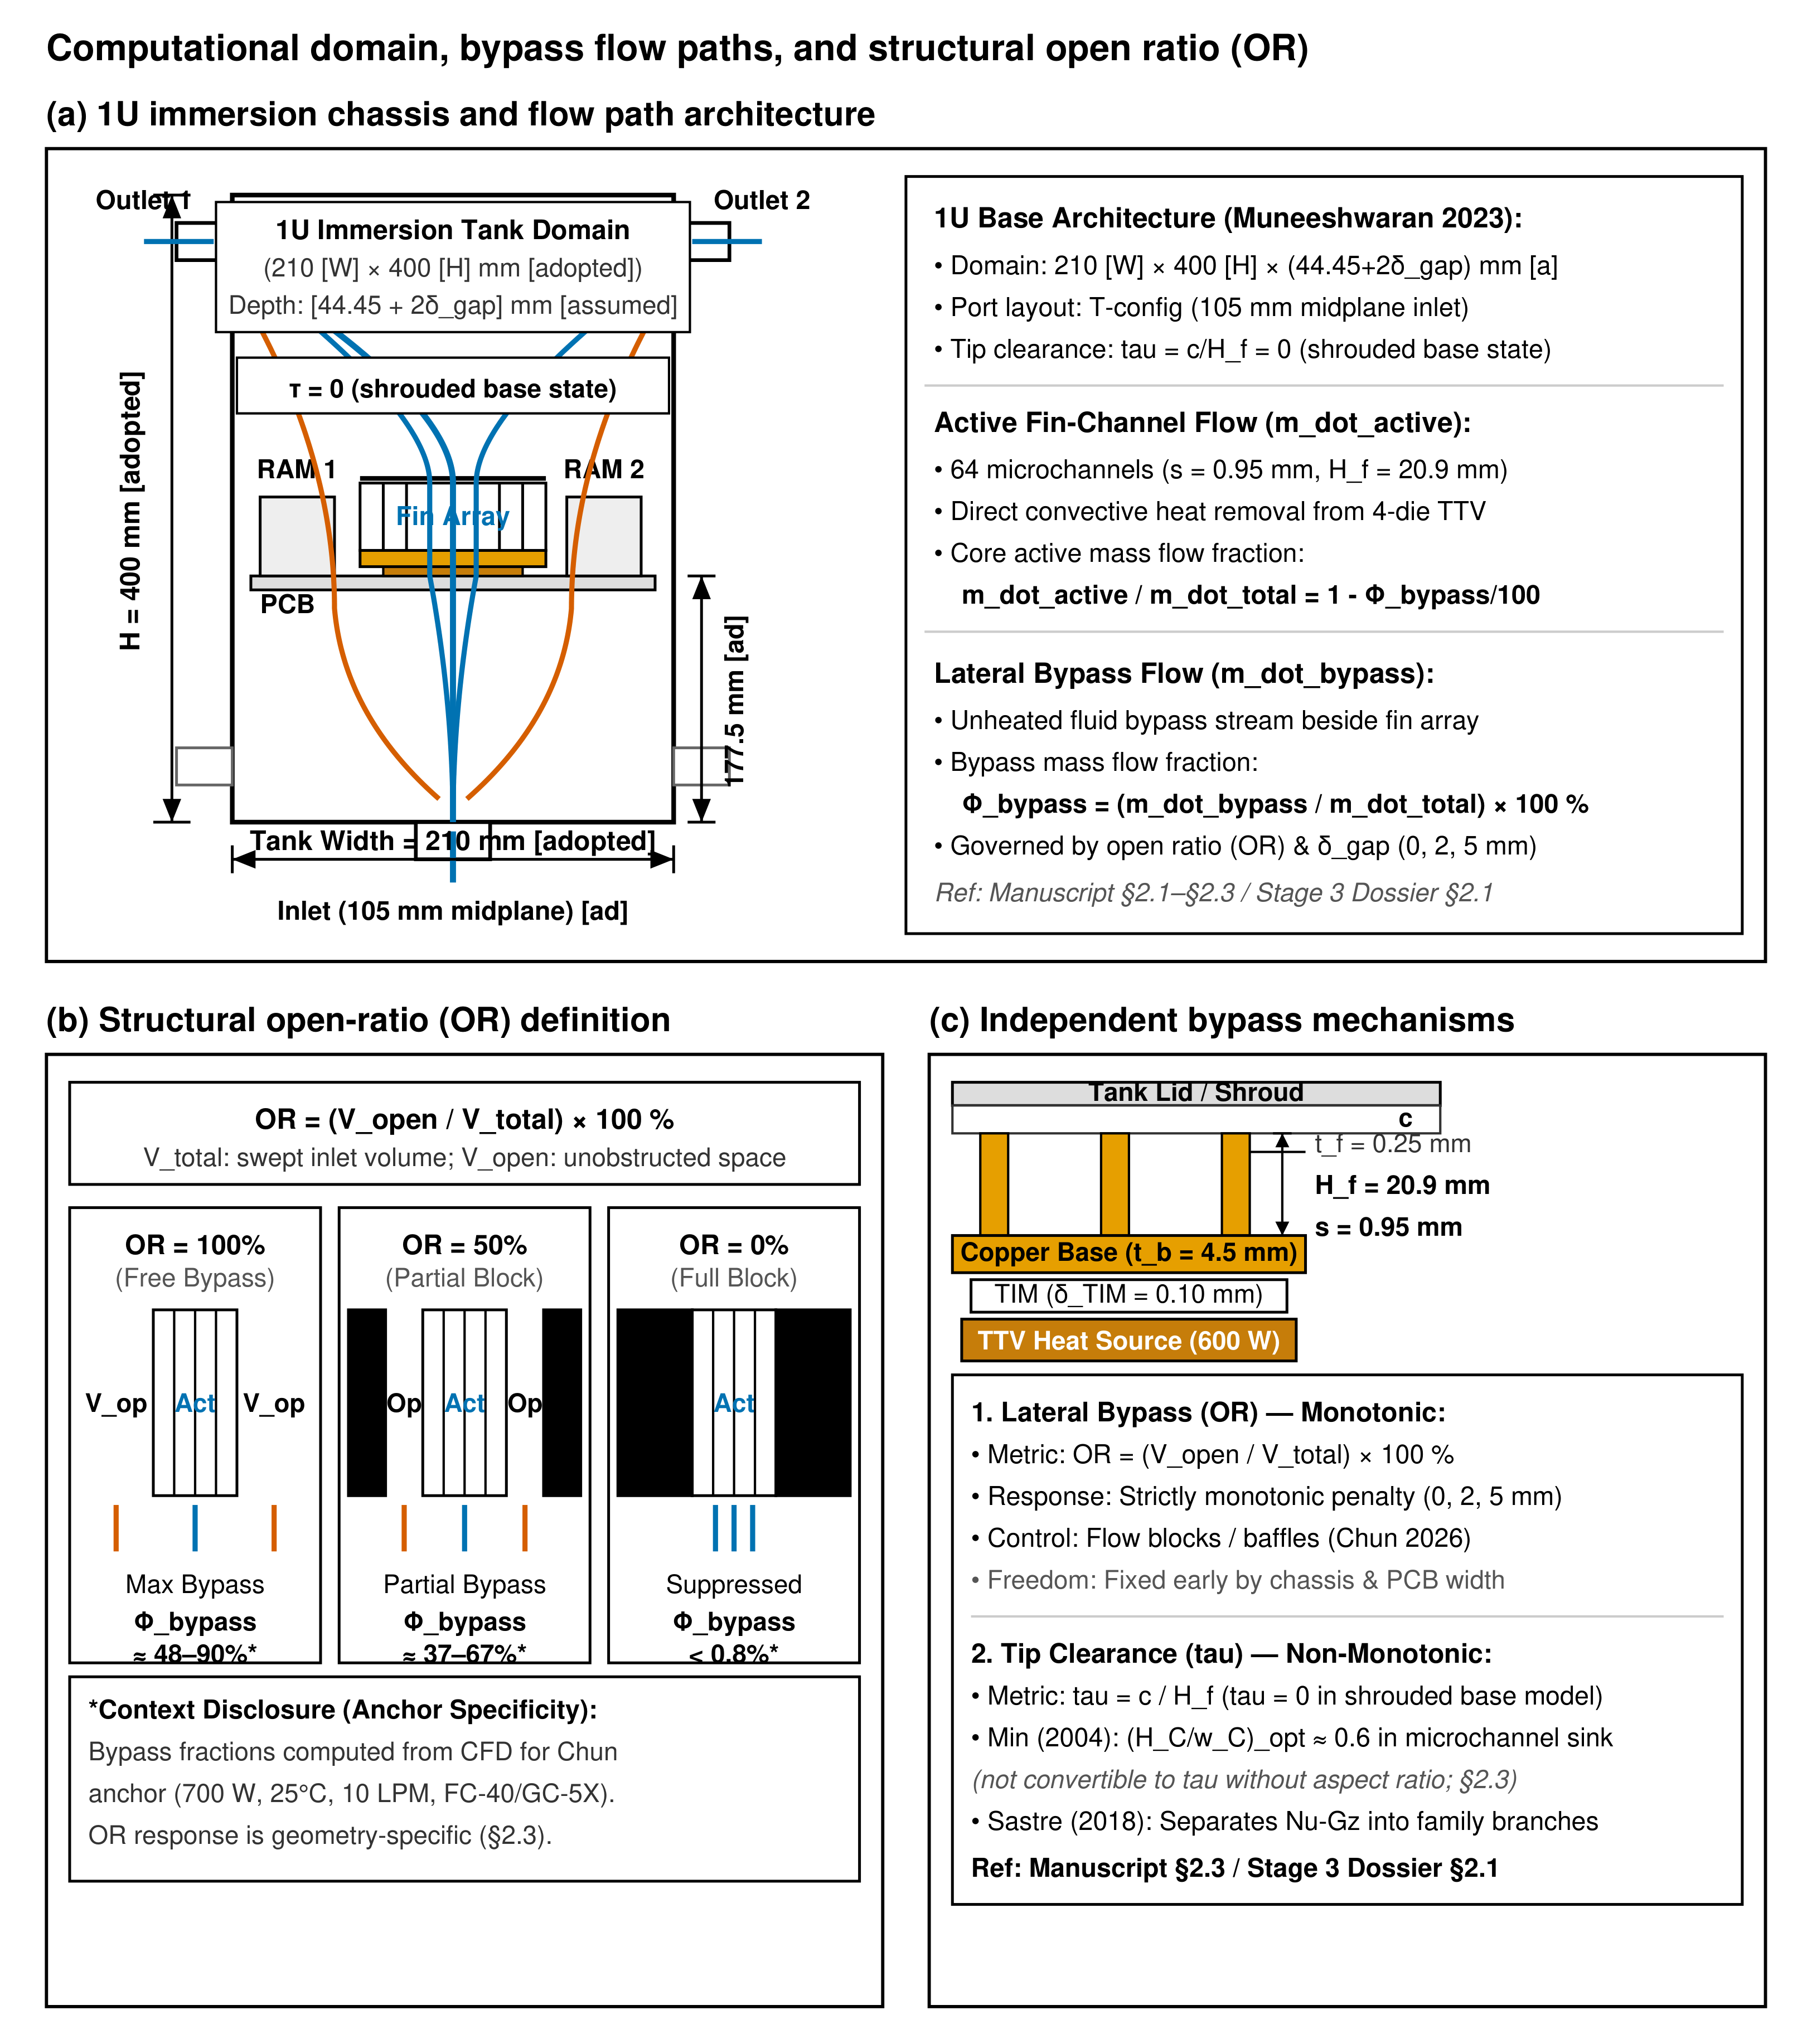
\includegraphics[width=\textwidth]{../figures/fig1_domain.png}
\caption{Computational domain, bypass flow paths and the open-ratio definition. (a) the 1U
immersion chassis with the active fin-channel flow and lateral bypass stream (with the shrouded
$\tau=0$ base state and independent tip clearance treated in panel (c)). (b) the open-ratio
definition at the heat-sink inlet plane across three blockage states. (c) lateral bypass and tip
clearance shown as the two independent mechanisms carried separately in this model, per
Section~\ref{sec:openratio}.}
\label{fig:domain}
\end{figure}

Table~\ref{tab:ledger-base} is the complete dimension ledger for the base model. Every row carries
one of three tags. A row tagged \texttt{[adopted]} is printed in the cited source at the cited
page, in body text, in a table, or as a dimension callout drawn on a figure. A row tagged
\texttt{[derived]} is computed from \texttt{[adopted]} rows, with the arithmetic shown. A row
tagged \texttt{[assumed]} is not available in any source consulted, and its value, its bounds and
the results it can move are stated in Section~\ref{sec:assumptions}. No row in the ledger is
digitised from a plot. Several of the \texttt{[adopted]} rows are recoverable only by rendering
the source page to an image and reading the drawing, because plain text extraction drops
dimension callouts that exist as vector labels inside a figure; those rows name the figure.

\begingroup
\footnotesize
\setlength{\tabcolsep}{4pt}
\begin{longtable}{@{}r>{\raggedright\arraybackslash}p{0.200\textwidth}c>{\raggedright\arraybackslash}p{0.135\textwidth}l>{\raggedright\arraybackslash}p{0.275\textwidth}@{}}
\caption{Dimension ledger for the base model, the 1U immersion server of Muneeshwaran et
al.~\cite{muneeshwaran2023}. Page numbers are the printed journal page of
\textit{Int.\ Commun.\ Heat Mass Transf.} \textbf{145} (2023) 106843, which coincides with the
PDF page index for this article.}
\label{tab:ledger-base}\\
\toprule
\# & Quantity & Symbol & Value & Tag & Source or arithmetic \\
\midrule
\endfirsthead
\multicolumn{6}{@{}l}{\normalfont\itshape Table~\ref{tab:ledger-base} continued}\\
\toprule
\# & Quantity & Symbol & Value & Tag & Source or arithmetic \\
\midrule
\endhead
\midrule
\multicolumn{6}{@{}r}{\normalfont\itshape continued on next page}\\
\endfoot
\bottomrule
\endlastfoot
1  & Rack unit height, server slot        &            & 44.45~mm & \texttt{[adopted]} & p.~1, abstract \\
2  & Heat-sink base thickness             & $t_b$      & 4.5~mm   & \texttt{[adopted]} & p.~3, \S2.1 \\
3  & Fin thickness                        & $t_f$      & 0.25~mm  & \texttt{[adopted]} & p.~3, \S2.1 \\
4  & Fin height                           & $H_f$      & 20.9~mm  & \texttt{[adopted]} & p.~3, \S2.1 \\
5  & Fin pitch, two builds                & $p_f$      & 1.2 and 2.2~mm & \texttt{[adopted]} & p.~3; Table~3, p.~7 \\
6  & Fin channel width                    & $s$        & 0.95~mm; 1.95~mm & \texttt{[derived]} & $s=p_f-t_f$ \\
7  & Channel hydraulic diameter           & $D_h$      & 1.817~mm; 3.567~mm & \texttt{[derived]} & $D_h=2sH_f/(s+H_f)$ \\
8  & Heat-sink stack height               & $t_b+H_f$  & 25.4~mm  & \texttt{[derived]} & $4.5+20.9$ \\
9  & Heat-sink base footprint             & $L\times W$& 118~mm $\times$ 78~mm & \texttt{[adopted]} & Fig.~2(b), p.~5, rendered callouts \\
10 & Raised finned-section callouts       &            & 81~mm and 31.2~mm & \texttt{[adopted]} & Fig.~2(b), p.~5. The drawing does not label which feature each callout terminates on \\
11 & Fin-bank plan area                   & $A_{bank}$ & 78~mm $\times$ 118~mm & \texttt{[assumed]} & Bounds 31.2 $\times$ 81~mm to 78 $\times$ 118~mm; see Section~\ref{sec:assumptions} \\
12 & Fin count, $p_f=1.2$~mm              & $N_f$      & 65 fins, 64 channels & \texttt{[derived]} & $Nt_f+(N-1)s=W$ on row 11 \\
13 & Fin count, $p_f=2.2$~mm              & $N_f$      & 36 fins, 35 channels & \texttt{[derived]} & same relation on row 11 \\
14 & Channel free-flow area, base build   & $A_c$      & $1.271\times10^{-3}$~m$^2$ & \texttt{[derived]} & $64\times0.95\times20.9$~mm$^2$ \\
15 & Heat-sink material                   &            & copper   & \texttt{[adopted]} & p.~3, \S2.1 \\
16 & Mock CPU package footprint           &            & 48~mm $\times$ 68~mm & \texttt{[adopted]} & Fig.~2(e), p.~7, rendered callouts \\
17 & Die count                            &            & 4, independently modulated & \texttt{[adopted]} & p.~3, \S2.1; Fig.~2(e), p.~7 \\
18 & Individual die footprint             &            & 2 $\times$ 2 tiling of a centred block & \texttt{[assumed]} & Bounds 50\% to 90\% of the package footprint; see Section~\ref{sec:assumptions} \\
19 & Thermal interface material           &            & grease TC-5888, $k=5.2$ &  \texttt{[adopted]} & p.~3, \S2.1; $k$ in W~m$^{-1}$~K$^{-1}$ \\
20 & TIM bond-line thickness              & $\delta_{TIM}$ & 0.10~mm & \texttt{[assumed]} & Bounds 0.05 to 0.20~mm; see Section~\ref{sec:assumptions} \\
21 & Bypass gap, heat sink to tank wall   & $\delta_{gap}$ & 0, 2, 5~mm & \texttt{[adopted]} & p.~5, \S3.2; Fig.~6, p.~9; Fig.~7, p.~10 \\
22 & Tank, long horizontal dimension      &            & 210~mm   & \texttt{[adopted]} & Fig.~2(c), p.~6, rendered callouts \\
23 & Tank, vertical dimension             &            & 400~mm   & \texttt{[adopted]} & Fig.~2(c), p.~6 \\
24 & Bottom inlet axis from tank end wall &            & 105~mm   & \texttt{[adopted]} & Fig.~2(c), p.~6; $105=210/2$, so the inlet is on the tank mid-plane \\
25 & Side port axes from floor and ceiling&            & 27.5~mm  & \texttt{[adopted]} & Fig.~2(c), p.~6 \\
26 & Heat-sink underside above tank floor &            & 177.5~mm & \texttt{[adopted]} & Fig.~2(c), p.~6 \\
27 & Tank depth, out-of-plane             &            & 44.45~mm internal $+\,2\delta_{gap}$ & \texttt{[assumed]} & Bounds 44.45 to 55~mm internal; see Section~\ref{sec:assumptions} \\
28 & Tank wall material                   &            & acrylic, adiabatic outer face & \texttt{[assumed]} & $k=0.19$; bounds 0.19 to 16.4~W~m$^{-1}$~K$^{-1}$; see Section~\ref{sec:assumptions} \\
29 & Server tray outline                  &            & 275 and 245~mm; 201 and 141.7~mm & \texttt{[adopted]} & Fig.~2(a), p.~5, rendered callouts \\
30 & Memory bank envelope                 &            & 149 $\times$ 59.3 $\times$ 34.1~mm; pitch 7.5~mm; gap 3.3~mm & \texttt{[adopted]} & Fig.~2(d), p.~6, rendered callouts \\
31 & Memory thermal load                  &            & zero, flow obstruction only & \texttt{[adopted]} & p.~3, \S2.1 \\
32 & PCB thickness                        &            & 2.4~mm   & \texttt{[assumed]} & From Khoshvaght-Aliabadi et al.~\cite{khoshvaghtaliabadi2026oblique}, Table~1, p.~5; bounds 1.6 to 3.0~mm \\
\end{longtable}
\endgroup

\begin{figure}[htbp]
\centering
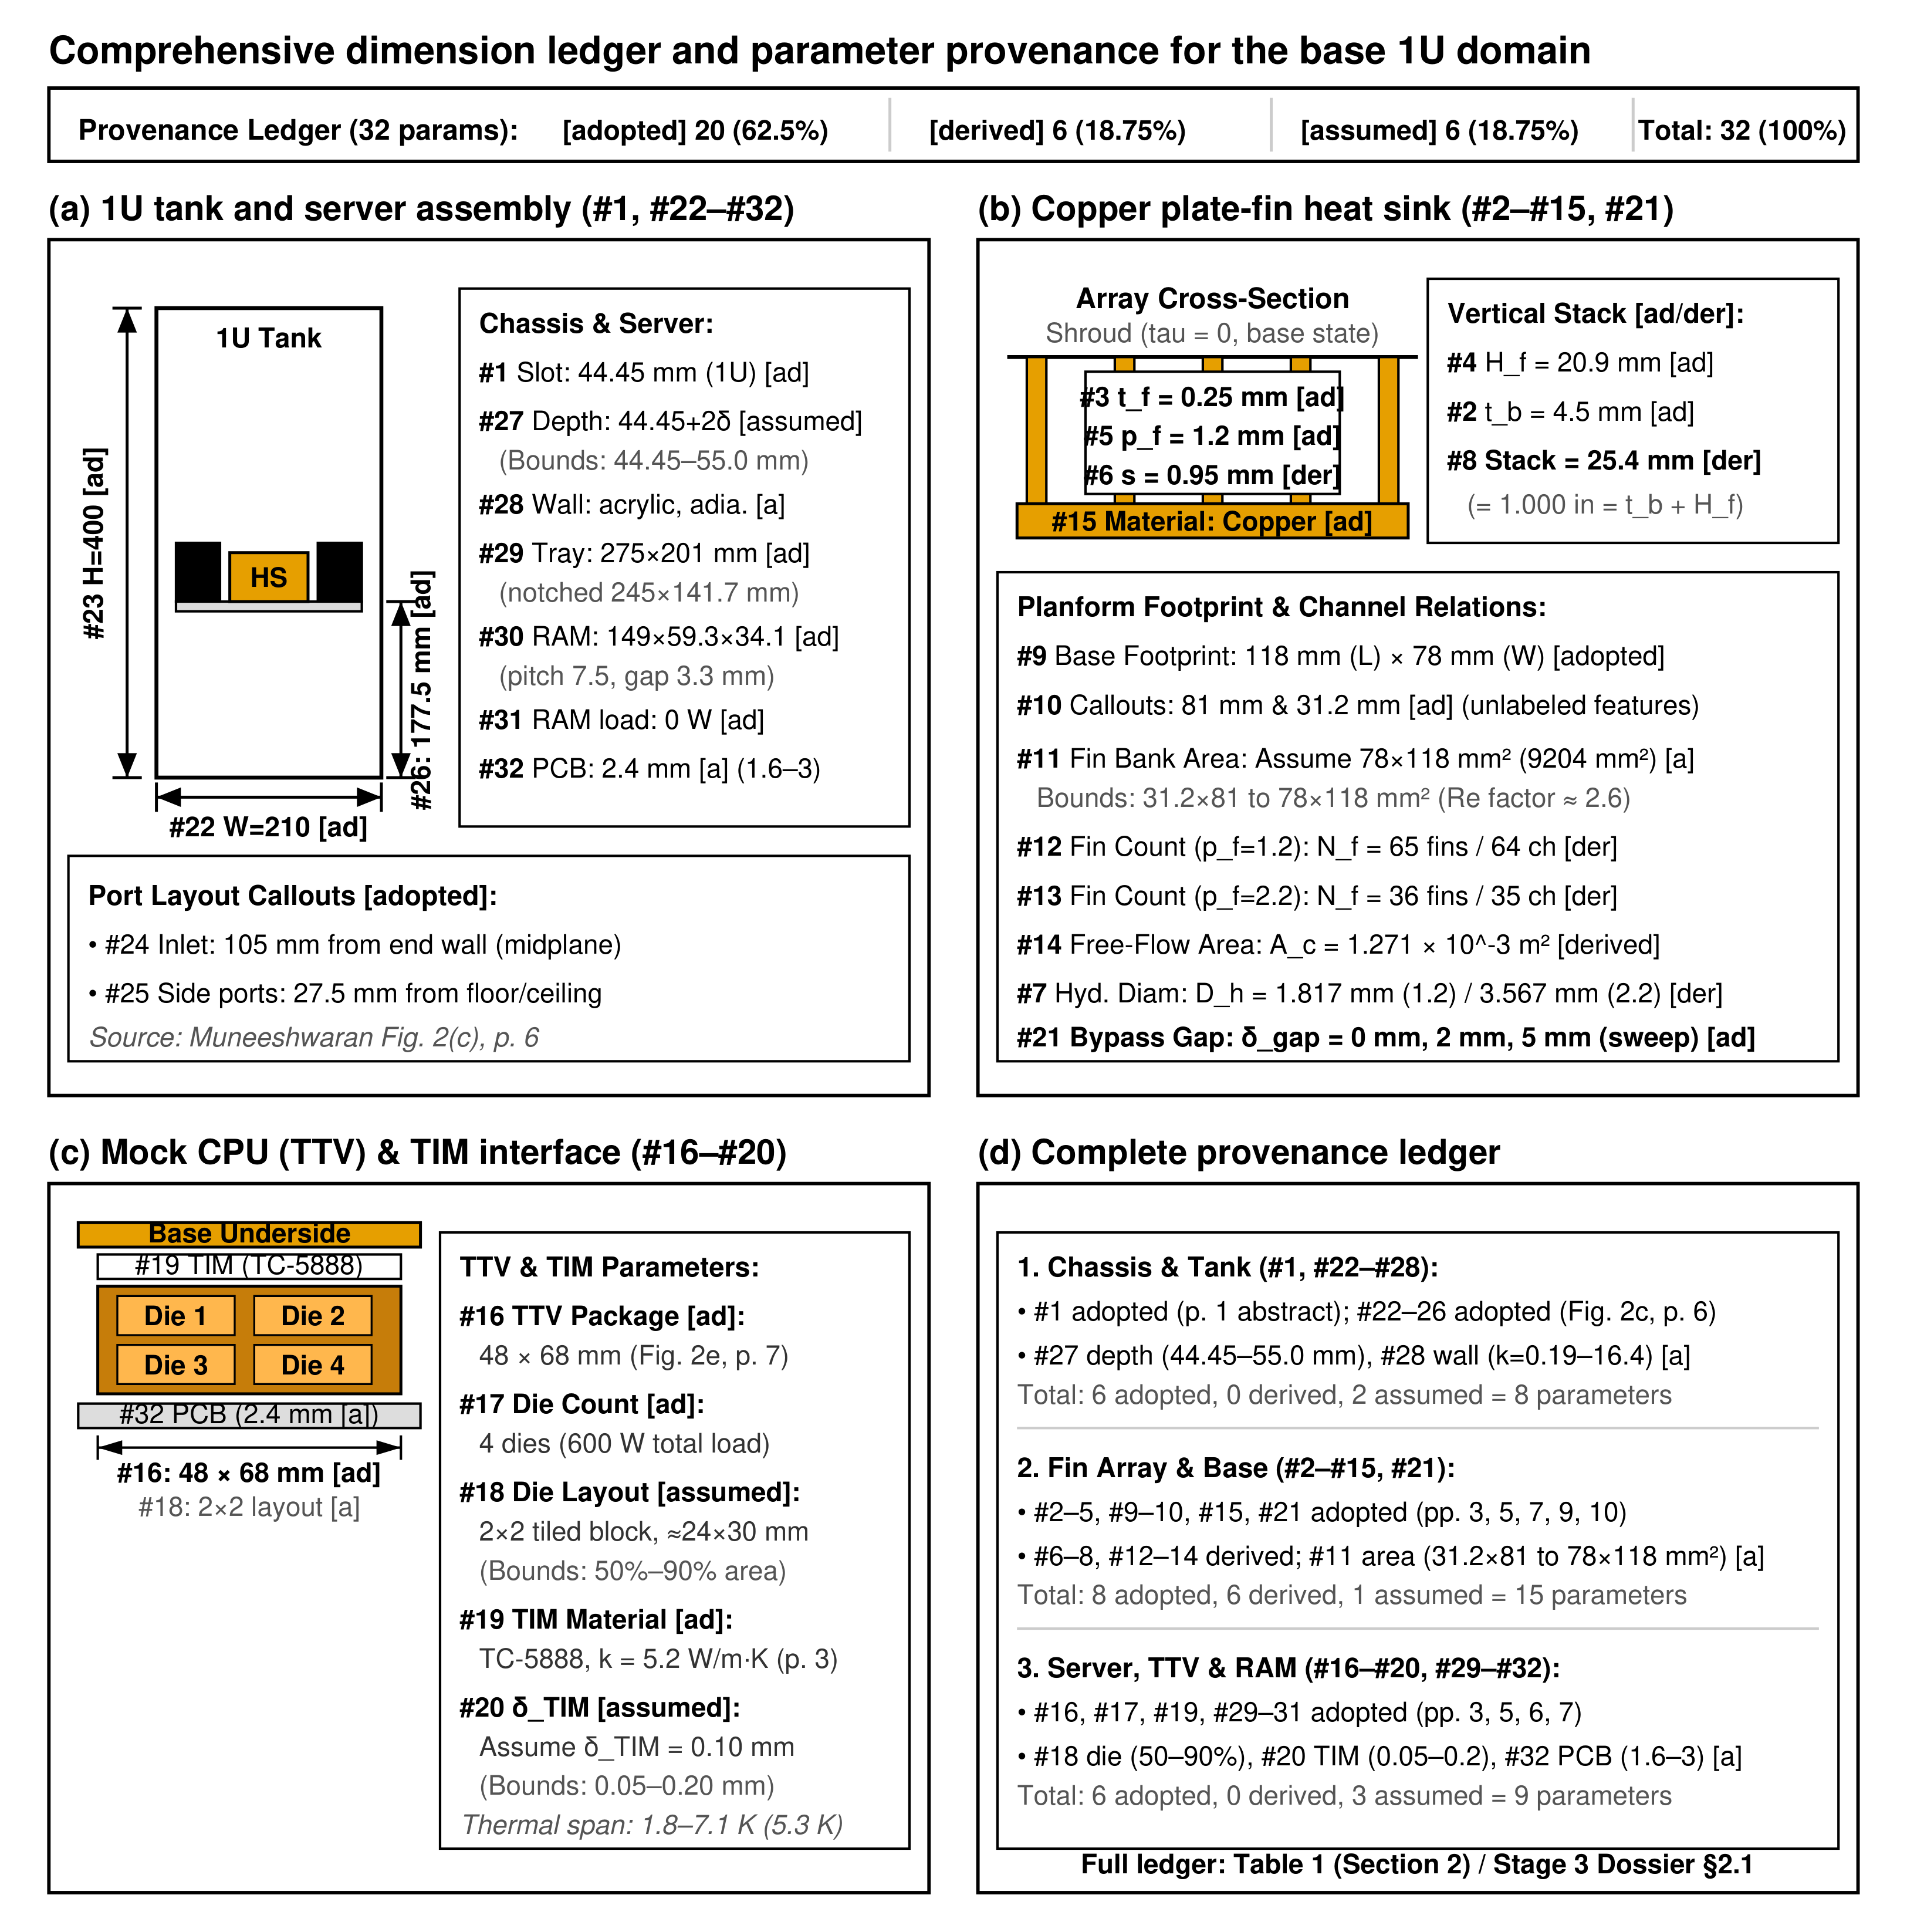
\includegraphics[width=\textwidth]{../figures/fig2_dimension_ledger.png}
\caption{Dimension ledger and parameter provenance for the base model geometry, matching
Table~\ref{tab:ledger-base}. Adopted, derived and assumed dimensions are visually distinguished
so that the source of every number in the model is visible at a glance.}
\label{fig:ledger}
\end{figure}

Two conventions follow from the ledger and are stated here so that no downstream quantity is
ambiguous. First, the fin bank is taken to span the 78~mm base width, so the span sets the channel
count and the 118~mm base length is the channel flow length. Second, the channel hydraulic
diameter of row 7 is the length scale for every Reynolds and Nusselt number reported in this
paper. That second point needs saying because the bypass and tip-clearance literature this work
builds on does not share a convention: Sastre et al.~\cite{sastre2018} use the hydraulic diameter
of the finned cross-section including the clearance slab, Mei et al.~\cite{mei2014} use the pin
diameter with the maximum velocity, Jeng~\cite{jeng2008} uses the bare rectangular duct with the
inlet velocity, Shahsavar et al.~\cite{shahsavar2021} use four times the array volume over its
wetted area, Shrigondekar et al.~\cite{shrigondekar2023} use the bare fin spacing, and Min et
al.~\cite{min2004} report no Reynolds number at all and sweep pumping power instead. Five
incompatible length scales across six papers is a large part of why no dimensionless framework for
this problem exists yet, and every literature value quoted in this paper is recomputed on the
convention above before it is compared with anything.

Applying that convention to the base geometry gives a channel Reynolds number
$\mathrm{Re}_{ch}=\dot{m}D_h/(A_c\mu)$ of roughly 5 to 122 over the 1 to 3~LPM flow range and the
15 to 35~$^{\circ}$C inlet range, if all flow is forced through the fins. The band is wide, and it
is wide for an honest reason: it carries the factor of about 2.6 between the two bounds of the
fin-bank span in row 11. No single-valued channel Reynolds number is quoted for the base geometry
anywhere in this paper. The one directly printed check available is Shrigondekar et
al.~\cite{shrigondekar2023}, who report a fin-spacing Reynolds number of about 10 to 70 for FC-40
on the same rig at the same flow rates and the same two fin pitches. Converted onto the fin-spacing
length scale, the wide-span bound of row 11 gives 2.5 to 46 and the narrow-span bound gives 6.4 to
114. The printed value therefore sits inside the narrow band and partly above the wide one, which
means this check leans against the value adopted rather than confirming it. That is recorded here
rather than smoothed over.

\subsection{Reference configuration for the anchor comparison}
\label{sec:v3}

A second, fully dimensioned geometry is carried alongside the base model so that the open-ratio
results of Chun et al.~\cite{chun2026} can be reproduced without rescaling anything.
Table~\ref{tab:ledger-v3} is its ledger. It is not a substitute for the base model and no result
from the two configurations is pooled.

\begingroup
\footnotesize
\setlength{\tabcolsep}{4pt}
\begin{longtable}{@{}l>{\raggedright\arraybackslash}p{0.225\textwidth}>{\raggedright\arraybackslash}p{0.185\textwidth}l>{\raggedright\arraybackslash}p{0.245\textwidth}@{}}
\caption{Dimension ledger for the reference configuration used in the anchor comparison, the 1U
plate-fin build of Chun et al.~\cite{chun2026}. Page numbers are the printed journal page of
\textit{Energy} \textbf{361} (2026) 141967.}
\label{tab:ledger-v3}\\
\toprule
\# & Quantity & Value & Tag & Source or arithmetic \\
\midrule
\endfirsthead
\multicolumn{5}{@{}l}{\normalfont\itshape Table~\ref{tab:ledger-v3} continued}\\
\toprule
\# & Quantity & Value & Tag & Source or arithmetic \\
\midrule
\endhead
\midrule
\multicolumn{5}{@{}r}{\normalfont\itshape continued on next page}\\
\endfoot
\bottomrule
\endlastfoot
A1  & 1U internal slot spacing        & 44.45~mm & \texttt{[adopted]} & p.~5, \S2.1 \\
A2  & Fin thickness                   & 2~mm     & \texttt{[adopted]} & Fig.~2(a), p.~5, callout under a ``Unit : mm'' header \\
A3  & Fin spacing                     & 3~mm     & \texttt{[adopted]} & Fig.~2(a), p.~5 \\
A4  & Fin height                      & 20~mm    & \texttt{[adopted]} & Fig.~2(a), p.~5 \\
A5  & Fin pitch                       & 5~mm     & \texttt{[derived]} & $2+3$ \\
A6  & Heat-sink base plate            & 72~mm width $\times$ 106~mm flow length & \texttt{[adopted]} & Fig.~2(a), p.~5 \\
A7  & Fin count                       & 15 fins, 14 channels & \texttt{[derived]} & $2N+3(N-1)=72$ gives $N=15$ exactly \\
A8  & Channel free-flow area          & $8.40\times10^{-4}$~m$^2$ & \texttt{[derived]} & $14\times3\times20$~mm$^2$ \\
A9  & Channel hydraulic diameter      & 5.217~mm & \texttt{[derived]} & $2(3)(20)/23$ \\
A10 & Copper block, mock CPU          & 50 $\times$ 65 $\times$ 8~mm & \texttt{[adopted]} & Fig.~2(a), p.~5 \\
A11 & TIM, indium foil thickness      & $\approx$0.1~mm & \texttt{[adopted]} & p.~6, \S2.1 \\
A12 & Heat-sink centre spacing on PCB & 60~mm    & \texttt{[adopted]} & p.~6, \S2.1, and Fig.~2(a), p.~5 \\
A13 & Tank internal width             & 423~mm   & \texttt{[adopted]} & Fig.~2(a), p.~5, right-hand panel headed ``Immersion tank'' \\
A14 & Tank internal height, outlet plane to distribution-plate plane & 430~mm & \texttt{[adopted]} & Fig.~2(a), p.~5, right-hand panel \\
A15 & Distribution plate, 1U build    & 10 holes, 10~mm diameter & \texttt{[adopted]} & p.~5, \S2.1 \\
A16 & Distribution plate, 3U build    & 30 holes, 5~mm diameter & \texttt{[adopted]} & p.~5, \S2.1 \\
A17 & Tank material                   & SUS304, double-layer insulation, tempered-glass window & \texttt{[adopted]} & p.~4, \S2.1; properties Table~2, p.~6 \\
A18 & Flow-control block material     & acrylic  & \texttt{[adopted]} & p.~6, \S2.1 \\
A19 & Flow-control block dimensions   & not dimensioned in the source & \texttt{[assumed]} & The open ratio is therefore defined here by the volume a block occludes, never by a block dimension \\
A20 & Tank external envelope          & not printed in the source & \texttt{[assumed]} & Not required: the computational domain is the wetted interior bounded by A13, A14 and A1 \\
A21 & Metal-foam alternative core     & 10~PPI, porosity 0.9; sweep 5 to 15~PPI, porosity 0.5 to 0.9 & \texttt{[adopted]} & p.~15 and p.~18, \S3.3 \\
\end{longtable}
\endgroup

Three specific gaps in this reference configuration are carried openly rather than closed
silently, because an independent reproducibility check found them and they are real. The source
does not print the tank's third, out-of-plane dimension, does not print the heat-sink base
thickness, and does not give the numerical inlet profile, outlet type or tank-wall thermal
condition, so the anchor comparison in Section~\ref{sec:verification} is a best-effort check
against a paper that does not fully close its own specification, not a fully reproducible
benchmark. The same three gaps are the reason A19, A20 and the base thickness never enter a
reported quantity.

\subsection{Open ratio}
\label{sec:openratio}

The bypass metric is adopted verbatim from Chun et al.~\cite{chun2026}, who introduce it as an
unnumbered display equation on their p.~11 and illustrate it in their Fig.~8. Their words for it,
quoted so that nothing is quietly reinterpreted here, are that the open ratio is
\textit{the volumetric fraction of the unobstructed fluid inlet space relative to the total heat
sink inlet volume}:

\begin{equation}
\mathrm{OR} = \frac{V_{\mathrm{open}}}{V_{\mathrm{total}}}\times 100 \quad (\%)
\label{eq:or}
\end{equation}

\noindent
Named for the geometry of Table~\ref{tab:ledger-base}, the two volumes in Eq.~(\ref{eq:or}) are
the following. $V_{\mathrm{total}}$ is the total heat-sink inlet volume, the fluid volume swept
out by the heat-sink inlet plane over the inlet-plane thickness, that is the plan area of the 1U
slot facing the heat sink multiplied by the inlet-plane thickness, spanning the full tank width
available to the flow at that height. $V_{\mathrm{open}}$ is the unobstructed fluid inlet space,
the part of $V_{\mathrm{total}}$ occupied by neither the heat sink nor a flow-control block, that
is the volume through which fluid can reach the outlets without passing between the fins. At
$\mathrm{OR}=100\%$ the tank is unobstructed and bypass is free. At $\mathrm{OR}=0\%$ every
entering parcel is directed through the heat-source region.

Three properties of the definition travel with it, because dropping any of them changes what the
number means. It is a volume ratio at the inlet plane, not an area ratio and not a clearance in
millimetres; the source never converts it to a gap width. It is geometry-specific, and the source
says so, so any open ratio quoted here travels with the geometry it was measured on. And the
blocking acts laterally, from both edges symmetrically, which in the 1U build means the top gap is
absent and the open ratio is a purely lateral quantity.

Open ratio is a geometric input. Its companion output, also taken from
Chun et al.~\cite{chun2026}, is the bypass mass fraction,

\begin{equation}
\dot{m}_{\mathrm{bypass}} = \dot{m}_{\mathrm{total}} - \dot{m}_{\mathrm{active}},
\qquad
\Phi_{\mathrm{bypass}} = \frac{\dot{m}_{\mathrm{bypass}}}{\dot{m}_{\mathrm{total}}}\times 100
\quad (\%),
\label{eq:phibypass}
\end{equation}

\noindent
where the bypass region is the flow region excluding the heat-sink passages and the region
directed toward the heat source. This paper reports $\mathrm{OR}$ as the design variable and
$\Phi_{\mathrm{bypass}}$ as the computed response, in the same pairing the source uses.

Lateral bypass and tip clearance are carried as two separate parameters and are never combined
into one scalar. The tip clearance ratio is defined as

\begin{equation}
\tau = \frac{c}{H_f},
\label{eq:tau}
\end{equation}

\noindent
the clearance height over the fin height, and is held at $\tau=0$ in the base configuration. Four
reasons keep the two apart. The 1U build that defines the open ratio has already eliminated the
top gap, so folding a tip term into it would redefine the source's own quantity while keeping its
name. No study surveyed here varies both mechanisms; every tip-clearance study varies only the tip
gap and both side-bypass studies vary only the side gap, so a combined ratio would be a quantity
with no supporting measurement anywhere. Jeng~\cite{jeng2008} argues the point directly, noting
that the tip gap dominates in magnitude and can be changed late in a design while the channel
width is fixed early by the board width, which in a 1U immersion chassis holds with extra force.
And the two responses have different shapes. Tip clearance is non-monotonic and has an interior
optimum: Min et al.~\cite{min2004} report a minimum thermal resistance of 0.058~$^{\circ}$C~W$^{-1}$
at a clearance-to-channel-width ratio of 0.6 under 2.27~W of pumping power, and Mei et
al.~\cite{mei2014} report the same competing-effects reversal. Lateral bypass is monotonic and
always detrimental, in Muneeshwaran et al.~\cite{muneeshwaran2023} across the 0 to 5~mm gap sweep
and in Chun et al.~\cite{chun2026} across the open-ratio sweep. Collapsing a bounded parameter
with an optimum and a monotone detrimental one into a single scalar would make any interior
optimum in the combined ratio unattributable to either mechanism. Sastre et al.~\cite{sastre2018}
supply the warning empirically: even one clearance parameter was strong enough to split their
Nusselt-Graetz curves into separate families rather than one fit.

One out-of-sample check on the open ratio exists and is used. Jeng~\cite{jeng2008} parameterises
lateral bypass around a square pin-fin sink as the ratio $W/L$ of channel width to sink length. For
a constant-height inlet plane the two parameterisations map exactly, $\mathrm{OR} = (1-L/W)\times
100$, so $W/L$ of 1, 2, 3 and 5 correspond to open ratios of 0, 50, 66.7 and 80\%. Jeng's
recommendation of $W/L$ between 2 and 3 therefore sits inside the range swept here, in a different
fluid and a different fin type. The mapping is derived here, not printed in either source, and it
holds only when the open volume is the lateral space at the same inlet-plane height.

\subsection{Working fluids and thermophysical properties}
\label{sec:properties}

Two dielectric coolants are used. FC-40, a perfluorinated fluorocarbon, is the primary fluid: it is
the one coolant for which more than one independent group in this literature has published usable
property data, so a property error can be caught by cross-checking rather than trusted. GC-5X, an
oil-based dielectric, is the high-viscosity contrast case. Carrying two fluids is not decoration.
Chun et al.~\cite{chun2026} show that open-ratio sensitivity is a strong function of viscosity,
with thermal resistance falling 6.1\% for FC-40 but 45.6\% for GC-5X as the bypass is closed, so a
framework claimed to be dimensionless must be exercised across more than one Prandtl decade or the
claim is untested.

Table~\ref{tab:fluidprops} gives the property treatment and the source of every value.

\begin{table}[htbp]
\centering
\caption{Coolant thermophysical properties and their sources. The correlations of Chun et
al.~\cite{chun2026} take $T$ in kelvin; see the discussion below.}
\label{tab:fluidprops}
\footnotesize
\setlength{\tabcolsep}{4pt}
\begin{tabular}{@{}l>{\raggedright\arraybackslash}p{0.105\textwidth}>{\raggedright\arraybackslash}p{0.405\textwidth}>{\raggedright\arraybackslash}p{0.215\textwidth}@{}}
\toprule
Fluid & Property & Value or correlation ($T$ in K) & Source \\
\midrule
FC-40 & $\rho$    & $2499 - 2.16\,T$~kg~m$^{-3}$ & \cite{chun2026}, Table~3, p.~7 \\
FC-40 & $k$       & $0.086 - 6.90\times10^{-5}\,T$~W~m$^{-1}$~K$^{-1}$ & \cite{chun2026}, Table~3, p.~7 \\
FC-40 & $c_p$     & $590 + 1.55\,T$~J~kg$^{-1}$~K$^{-1}$ & \cite{chun2026}, Table~3, p.~7 \\
FC-40 & $\mu$     & $0.0429 - 0.162\times10^{-3}\,T$ $+\;1.08\times10^{-7}\,T^2$~Pa~s & \cite{chun2026}, Table~3, p.~7 \\
FC-40 & $\rho$ & 1874.44~kg~m$^{-3}$ at 16~$^{\circ}$C & \cite{muneeshwaran2023}, Table~4, p.~7 \\
FC-40 & $\nu$ & $5\times10^{-6}$, $1.5\times10^{-6}$, $5.4\times10^{-7}$~m$^2$~s$^{-1}$ at 0, 40, 100~$^{\circ}$C & \cite{muneeshwaran2023}, Table~4, p.~7 \\
FC-40 & $c_p$ & 1014, 1076, 1169.4~J~kg$^{-1}$~K$^{-1}$ at 0, 40, 100~$^{\circ}$C & \cite{muneeshwaran2023}, Table~4, p.~7 \\
FC-40 & $k$ & 0.067, 0.0642, 0.0601~W~m$^{-1}$~K$^{-1}$ at 0, 40, 100~$^{\circ}$C & \cite{muneeshwaran2023}, Table~4, p.~7 \\
FC-40 & $\beta$   & $1.2\times10^{-3}$~K$^{-1}$ & \cite{muneeshwaran2023}, Table~4, p.~7 \\
FC-40 & Boiling pt. & 165~$^{\circ}$C at 1~bar & \cite{muneeshwaran2023}, Table~4, p.~7 \\
FC-40 & $\mathrm{Pr}$ & 67.5 at 25~$^{\circ}$C & \texttt{[derived]} from the correlations above \\
\midrule
GC-5X & $\rho$    & $1049.862 - 0.75\,T$~kg~m$^{-3}$ & \cite{chun2026}, Table~3, p.~7 \\
GC-5X & $k$       & $0.199367 - 1.8\times10^{-4}\,T$~W~m$^{-1}$~K$^{-1}$ & \cite{chun2026}, Table~3, p.~7 \\
GC-5X & $c_p$     & $2076.055 + 0.3\,T$~J~kg$^{-1}$~K$^{-1}$ & \cite{chun2026}, Table~3, p.~7 \\
GC-5X & $\mu$     & $0.6449 - 4.1234\times10^{-3}\,T$ $+\;8.9697\times10^{-6}\,T^2$ $-\;6.5833\times10^{-9}\,T^3$~Pa~s & \cite{chun2026}, Table~3, p.~7 \\
GC-5X & $\beta$   & $9.08\times10^{-4}$~K$^{-1}$ at 25~$^{\circ}$C & \texttt{[derived]}, $\beta=-\rho^{-1}\partial\rho/\partial T$ on the density fit of this table. No measured value is printed in any source consulted \\
GC-5X & $\mathrm{Pr}$ & 570 at 25~$^{\circ}$C & \texttt{[derived]} from the correlations above \\
\bottomrule
\end{tabular}
\end{table}

Two findings about these properties came out of checking them rather than copying them, and both
change how the correlations may be used.

The first is that the correlations of Chun et al.~\cite{chun2026} take $T$ in kelvin, which their
paper does not state and their own nomenclature contradicts by defining $T$ in degrees Celsius.
The evidence is arithmetic and it is decisive. With $T$ in kelvin the FC-40 density fit returns
1874.4~kg~m$^{-3}$ at 289.15~K, against the 1874.44~kg~m$^{-3}$ at 16~$^{\circ}$C measured
independently by Muneeshwaran et al.~\cite{muneeshwaran2023}. The conductivity fit returns 0.0672,
0.0644 and 0.0603~W~m$^{-1}$~K$^{-1}$ at 0, 40 and 100~$^{\circ}$C against their printed 0.067,
0.0642 and 0.0601, and the specific-heat fit returns 1013.4, 1075.4 and 1168.4~J~kg$^{-1}$~K$^{-1}$
against their printed 1014, 1076 and 1169.4. Three properties agree to better than 0.1\% at three
temperatures each on one unit convention and are irreconcilable on the other. The same conclusion
follows independently from the source's own mass-flow table, which converts to exactly 5.00~LPM per
heat sink at the stated 10~LPM for two heat sinks only when the density is evaluated in kelvin.
This is an inference from the paper's numbers, not a printed statement, and it should be confirmed
with the corresponding author before any anchor result is reproduced.

The second finding is a limit on the FC-40 viscosity fit, and it constrains the model. That
quadratic reaches zero at about 343~K, or 70~$^{\circ}$C, and is negative above it, so it cannot be
used at wall temperatures approaching the 80~$^{\circ}$C case-temperature limit of the base
paper~\cite{muneeshwaran2023}. Within its useful band it is good: against the kinematic-viscosity
points of Muneeshwaran et al.\ interpolated logarithmically it agrees to 1.2\% at 35~$^{\circ}$C
and 3.9\% at 25~$^{\circ}$C, degrading to 13\% at 15~$^{\circ}$C and 30\% at 0~$^{\circ}$C. FC-40
viscosity is therefore evaluated from the fit between 20 and 60~$^{\circ}$C and from the measured
points of Muneeshwaran et al.\ outside that band. The GC-5X cubic stays positive and monotone
across the whole range of interest and needs no such restriction.

Solid properties are listed in Table~\ref{tab:solidprops}. Where two sources print a value, both
are named, and where they agree exactly that is said, because agreement between independently
published tables is the only property check available in the absence of a measurement of our own.

\begin{table}[htbp]
\centering
\caption{Solid domain properties and their sources. Density in kg~m$^{-3}$, specific heat in J~kg$^{-1}$~K$^{-1}$, thermal conductivity in W~m$^{-1}$~K$^{-1}$.}
\label{tab:solidprops}
\footnotesize
\setlength{\tabcolsep}{4pt}
\begin{tabular}{@{}>{\raggedright\arraybackslash}p{0.155\textwidth}cc>{\raggedright\arraybackslash}p{0.105\textwidth}>{\raggedright\arraybackslash}p{0.30\textwidth}@{}}
\toprule
Domain & $\rho$ & $c_p$ & $k$ & Source \\
\midrule
Copper, fins and base & 8978 & 381 & 387.6 & \cite{chun2026}, Table~2, p.~6; the identical triplet is printed independently in \cite{khoshvaghtaliabadi2026oblique}, Table~1, p.~5 \\
TIM, base model, thermal grease & \multicolumn{2}{c}{not printed} & 5.2 & \cite{muneeshwaran2023}, p.~3, \S2.1 \\
TIM, reference configuration, indium & 7310 & 234 & 81.8 & \cite{chun2026}, Table~2, p.~6 \\
PCB substrate & 1850 & 1000 & 0.3 & \cite{khoshvaghtaliabadi2026oblique}, Table~1, p.~5 \\
PCB substrate, alternative & 3600 & 720 & 42.0 in-plane, 0.5 cross-plane & \cite{chun2026}, Table~2, p.~6 \\
SUS304, reference configuration tank & 8000 & 500 & 16.4 & \cite{chun2026}, Table~2, p.~6 \\
Acrylic, flow-control block and tank wall & 1180 & 1460 & 0.21 & \cite{chun2026}, Table~2, p.~6 \\
\bottomrule
\end{tabular}
\end{table}

The two PCB entries disagree by two orders of magnitude in conductivity because they describe
different things: one is an isotropic bulk laminate value, the other resolves the copper-plane
anisotropy. The isotropic entry is used for the base model, where the board is an unloaded
conduction path, and the anisotropic entry is used for the anchor comparison so that the
reference configuration keeps its own source's convention. Neither value moves a reported quantity
in this work, since the board carries no thermal load in the base model. All solid property values
in Table~\ref{tab:solidprops} are attributed within their source to further references rather than
measured there, and are carried on that basis.

\subsection{Assumptions}
\label{sec:assumptions}

Eight quantities in Tables~\ref{tab:ledger-base} and \ref{tab:ledger-v3} are not available in any
source consulted. Each is listed below with the value taken, the reason, the defensible bounds and
the results it can move. Nothing here is assumed because it was convenient, and nothing that a
result depends on is hidden inside a sentence.

\noindent\textbf{Fin-bank plan area, 78~mm $\times$ 118~mm (row 11).}\ The base outline of the heat sink is
dimensioned but the drawing does not label which feature its two interior callouts, 81~mm and
31.2~mm, terminate on. Bounds are therefore 31.2 $\times$ 81~mm at the low end and 78 $\times$
118~mm at the high end, a factor of 3.6 in plan area. The wide value is taken because it is the
only one under which the 48 $\times$ 68~mm mock-processor footprint of row 16 is fully covered by
the fin array. The counter-evidence is stated in Section~\ref{sec:geometry} and is not resolved:
converting the printed fin-spacing Reynolds range of Shrigondekar et al.~\cite{shrigondekar2023}
onto this geometry leans toward the narrow bound. Results moved: the span sets the channel count,
64 channels at 78~mm against 25 at 31.2~mm, hence a free-flow area of 1271~mm$^2$ against
496~mm$^2$, a factor of about 2.6 on channel velocity and on channel Reynolds number. Every
Reynolds number quoted for the base model carries that factor as a band. Thermal resistance is far
less sensitive, since the area enters through fin efficiency and total wetted area rather than
linearly. This is the largest single geometric uncertainty in the model, and the cheapest way to
settle it is a higher-resolution copy of the source drawing or a question to its corresponding
author.

\noindent\textbf{Die partition inside the mock-processor package (row 18).}\ The four dies are drawn as a
tiled block but the block is not dimensioned. Bounds are a die block between 50\% and 90\% of the
48 $\times$ 68~mm package footprint. The assumption is low-risk because the heat load is applied as
a boundary condition at the heat-sink base, following the base paper's own numerical
treatment~\cite{muneeshwaran2023}, so the die partition never enters the model. Results moved: only
a local peak junction temperature post-process, which this paper does not report.

\noindent\textbf{TIM bond-line thickness, 0.10~mm (row 20).}\ The base paper names the grease and gives its
conductivity but not the bond line. The value is set to match the indium-foil thickness printed for
the reference configuration~\cite{chun2026} so that both configurations share one interface
convention. Bounds 0.05 to 0.20~mm, the usual range for a screwed-down grease line. Results moved:
absolute case temperature shifts by about 5.3~K across those bounds ($-1.8$~K to $+3.5$~K relative to
the 0.10~mm nominal) at 600~W over the row 16 footprint. Thermal-resistance differences between open
ratios are insensitive to it, because it is a series resistance common to every case.

\noindent\textbf{Tank depth, 44.45~mm internal plus twice the bypass gap (row 27).}\ Genuinely absent. The tank
drawing carries no callout for the out-of-plane thickness and the body text gives none. The value
is chosen so that the tank interior is exactly the 1U slot the source's own abstract specifies.
Bounds 44.45 to 55~mm internal. Results moved: this dimension sets the bypass area and therefore
is the open ratio. It is the most consequential assumption in the ledger, and it is precisely why
this paper parameterises on the dimensionless open ratio rather than on an absolute tank depth.

\noindent\textbf{Tank wall material and outer boundary (row 28).}\ The base paper never names the tank material.
Acrylic with $k = 0.19$~W~m$^{-1}$~K$^{-1}$ is taken, consistent with the transparent wall in the
source's own photograph, with an adiabatic outer face. Bounds on $k$ run from 0.19 for acrylic to
16.4~W~m$^{-1}$~K$^{-1}$ for the stainless steel used in the reference
configuration~\cite{chun2026}. Results moved: none of those reported. The adiabatic outer face is
the source's own stated condition, since it reports that the entire experimental system was
insulated and that the heat loss was negligible~\cite{muneeshwaran2023}.

\noindent\textbf{PCB thickness, 2.4~mm (row 32).}\ Not given by the base paper. Taken from the only printed
PCB thickness available for a 1U immersion server~\cite{khoshvaghtaliabadi2026oblique}. Bounds 1.6
to 3.0~mm. Results moved: none reported here; the board is an unloaded conduction path of
$k \approx 0.3$~W~m$^{-1}$~K$^{-1}$.

\noindent\textbf{Flow-control block dimensions in the reference configuration (row A19).}\ The blocks are shown
schematically in the source but given no size. The open ratio is therefore defined by the volume a
block occludes, as in Eq.~(\ref{eq:or}), never by a block dimension. Results moved: the mapping
from open ratio to bypass fraction. Since this paper reports the open ratio as an input and the
bypass fraction as a computed output, no reported quantity requires the block geometry.

\noindent\textbf{External tank envelope in the reference configuration (row A20).}\ Not printed. Not required,
because the computational domain is the wetted interior bounded by rows A13, A14 and A1.

A separate set of quantities is held fixed rather than assumed, and each is fixed for a stated
reason. The rack unit height is held at 44.45~mm because it is an industry dimensional standard
printed identically by three independent groups~\cite{muneeshwaran2023,chun2026,kim2025}; it is not
a free design variable, and Kim et al.\ already swept it from 0.8U to 1.2U if a sensitivity
precedent is wanted. The mock-processor footprint is held at 48 $\times$ 68~mm because fixing the
heat-source footprint is what makes the open ratio the only varying geometric quantity; if the
footprint moved, a change in thermal resistance could not be attributed to bypass. The heat-sink
base thickness is held at 4.5~mm because it sets spreading resistance, which sits in series with
the convective resistance the open ratio acts on, so holding it keeps the two separable. The fin
material is held at copper: with a solid-to-fluid conductivity ratio near 6000 for FC-40, fin
efficiency is near unity and the result is insensitive to the copper grade, whereas switching to
aluminium would change fin efficiency and confound the bypass conclusion. The port arrangement is
held at the T-configuration because the base paper shows it is a first-order effect, 12.6\% in
thermal resistance against the Z-configuration, and because under the Z-configuration most of the
fluid bypasses the heat sink anyway; holding it removes a competing bypass mechanism so that the
open ratio is the only one varied~\cite{muneeshwaran2023}.

Fin pitch is deliberately not held constant. It is a second factor at the two printed levels of
1.2 and 2.2~mm, because the pitch and bypass interact: the penalty for opening the gap from 0 to
5~mm is 3\% at the coarse pitch but 7.4\% at the fine one~\cite{muneeshwaran2023}. The coolant is
deliberately not held constant either, for the Prandtl-range reason given in
Section~\ref{sec:properties}.
.
%
% PACKAGES REQUIRED IN main.tex PREAMBLE (not currently present):
%   \usepackage{booktabs}
%   \usepackage{array}      (for the >{\raggedright\arraybackslash}p{} column type)
% =============================================================================

\section{Problem formulation}
\label{sec:formulation}

\subsection{Base geometry}
\label{sec:geometry}

The model geometry is the 1U immersion server of Muneeshwaran et al.~\cite{muneeshwaran2023}:
a copper plate-fin heat sink clamped to a four-die thermal test vehicle on a printed circuit
board, with a bank of non-dissipating memory modules alongside it, the whole tray submerged in a
sealed 1U tank. Coolant enters through a port on the tank floor directly beneath the heat sink
and leaves through two ports at the top of the opposite faces, the arrangement those authors call
the T-configuration. That choice of base is not a matter of taste. It is the only 1U immersion
architecture in the surveyed literature whose server tray, heat sink, tank, memory bank and mock
processor all carry printed dimension callouts, so the domain can be rebuilt without scaling
anything off a figure. It is also the architecture that Chun et al.~\cite{chun2026} identify as
prior bypass-control work, that B. Zhang et al.~\cite{zhang2026} state they reconstructed as their
own computational domain, that Khoshvaght-Aliabadi and co-workers rebuilt twice as a validation
replica~\cite{khoshvaghtaliabadi2026oblique,khoshvaghtaliabadi2026component}, and from which Kim
et al.~\cite{kim2025} took their inlet and outlet arrangement. Only the first of those four is a
reuse of the architecture as a study domain; the others are weaker forms of reliance and are
described here as such.

The bypass mechanism this paper is about is present in the base paper and was measured there.
Muneeshwaran et al.~\cite{muneeshwaran2023} swept the clearance between the heat sink and the 1U
tank inner wall at 5, 2 and 0~mm, reported a 3\% to 7.4\% rise in thermal resistance and a
0.7~$^{\circ}$C to 1.5~$^{\circ}$C rise in case temperature as the gap opened, and adopted the
no-gap build for everything that followed. Their flow visualisation shows the reason: fluid takes
the clearance because its hydraulic resistance is lower, and that stream does no useful heat
transfer. The open ratio of Section~\ref{sec:openratio} is the dimensionless generalisation of
exactly this clearance.

\begin{figure}[htbp]
\centering
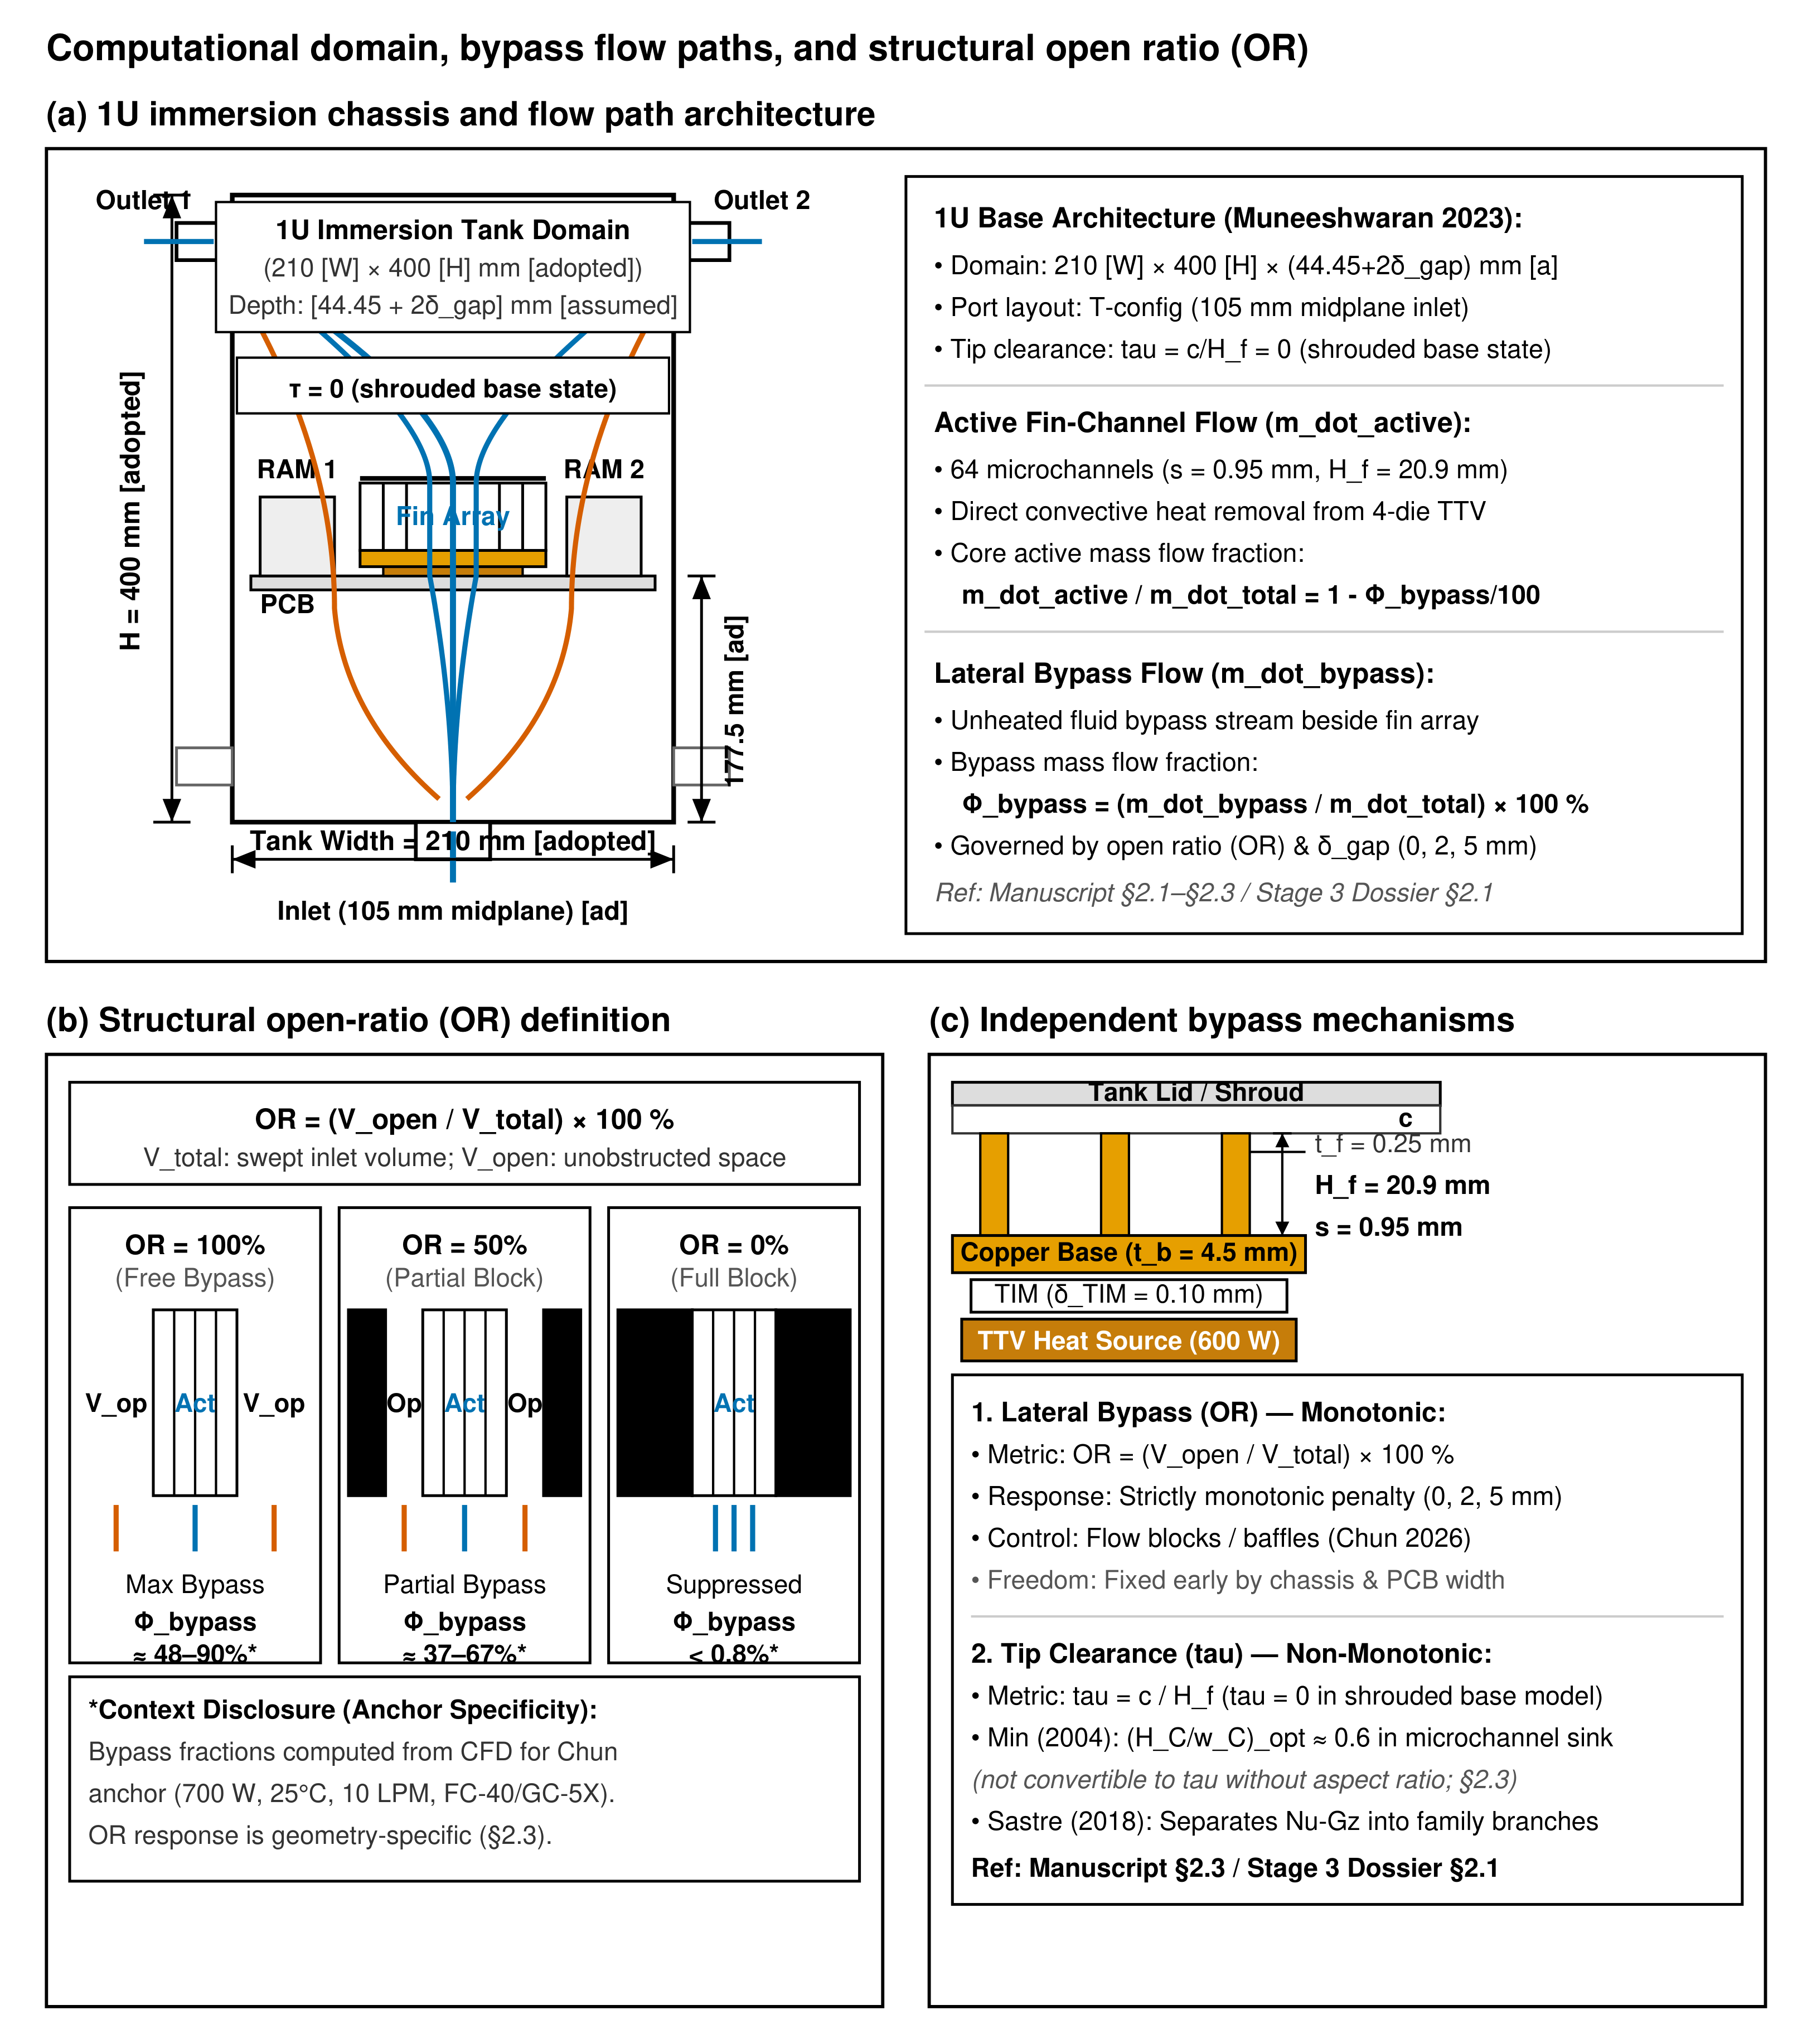
\includegraphics[width=\textwidth]{../figures/fig1_domain.png}
\caption{Computational domain, bypass flow paths and the open-ratio definition. (a) the 1U
immersion chassis with the active fin-channel flow and lateral bypass stream (with the shrouded
$\tau=0$ base state and independent tip clearance treated in panel (c)). (b) the open-ratio
definition at the heat-sink inlet plane across three blockage states. (c) lateral bypass and tip
clearance shown as the two independent mechanisms carried separately in this model, per
Section~\ref{sec:openratio}.}
\label{fig:domain}
\end{figure}

Table~\ref{tab:ledger-base} is the complete dimension ledger for the base model. Every row carries
one of three tags. A row tagged \texttt{[adopted]} is printed in the cited source at the cited
page, in body text, in a table, or as a dimension callout drawn on a figure. A row tagged
\texttt{[derived]} is computed from \texttt{[adopted]} rows, with the arithmetic shown. A row
tagged \texttt{[assumed]} is not available in any source consulted, and its value, its bounds and
the results it can move are stated in Section~\ref{sec:assumptions}. No row in the ledger is
digitised from a plot. Several of the \texttt{[adopted]} rows are recoverable only by rendering
the source page to an image and reading the drawing, because plain text extraction drops
dimension callouts that exist as vector labels inside a figure; those rows name the figure.

\begingroup
\footnotesize
\setlength{\tabcolsep}{4pt}
\begin{longtable}{@{}r>{\raggedright\arraybackslash}p{0.200\textwidth}c>{\raggedright\arraybackslash}p{0.135\textwidth}l>{\raggedright\arraybackslash}p{0.275\textwidth}@{}}
\caption{Dimension ledger for the base model, the 1U immersion server of Muneeshwaran et
al.~\cite{muneeshwaran2023}. Page numbers are the printed journal page of
\textit{Int.\ Commun.\ Heat Mass Transf.} \textbf{145} (2023) 106843, which coincides with the
PDF page index for this article.}
\label{tab:ledger-base}\\
\toprule
\# & Quantity & Symbol & Value & Tag & Source or arithmetic \\
\midrule
\endfirsthead
\multicolumn{6}{@{}l}{\normalfont\itshape Table~\ref{tab:ledger-base} continued}\\
\toprule
\# & Quantity & Symbol & Value & Tag & Source or arithmetic \\
\midrule
\endhead
\midrule
\multicolumn{6}{@{}r}{\normalfont\itshape continued on next page}\\
\endfoot
\bottomrule
\endlastfoot
1  & Rack unit height, server slot        &            & 44.45~mm & \texttt{[adopted]} & p.~1, abstract \\
2  & Heat-sink base thickness             & $t_b$      & 4.5~mm   & \texttt{[adopted]} & p.~3, \S2.1 \\
3  & Fin thickness                        & $t_f$      & 0.25~mm  & \texttt{[adopted]} & p.~3, \S2.1 \\
4  & Fin height                           & $H_f$      & 20.9~mm  & \texttt{[adopted]} & p.~3, \S2.1 \\
5  & Fin pitch, two builds                & $p_f$      & 1.2 and 2.2~mm & \texttt{[adopted]} & p.~3; Table~3, p.~7 \\
6  & Fin channel width                    & $s$        & 0.95~mm; 1.95~mm & \texttt{[derived]} & $s=p_f-t_f$ \\
7  & Channel hydraulic diameter           & $D_h$      & 1.817~mm; 3.567~mm & \texttt{[derived]} & $D_h=2sH_f/(s+H_f)$ \\
8  & Heat-sink stack height               & $t_b+H_f$  & 25.4~mm  & \texttt{[derived]} & $4.5+20.9$ \\
9  & Heat-sink base footprint             & $L\times W$& 118~mm $\times$ 78~mm & \texttt{[adopted]} & Fig.~2(b), p.~5, rendered callouts \\
10 & Raised finned-section callouts       &            & 81~mm and 31.2~mm & \texttt{[adopted]} & Fig.~2(b), p.~5. The drawing does not label which feature each callout terminates on \\
11 & Fin-bank plan area                   & $A_{bank}$ & 78~mm $\times$ 118~mm & \texttt{[assumed]} & Bounds 31.2 $\times$ 81~mm to 78 $\times$ 118~mm; see Section~\ref{sec:assumptions} \\
12 & Fin count, $p_f=1.2$~mm              & $N_f$      & 65 fins, 64 channels & \texttt{[derived]} & $Nt_f+(N-1)s=W$ on row 11 \\
13 & Fin count, $p_f=2.2$~mm              & $N_f$      & 36 fins, 35 channels & \texttt{[derived]} & same relation on row 11 \\
14 & Channel free-flow area, base build   & $A_c$      & $1.271\times10^{-3}$~m$^2$ & \texttt{[derived]} & $64\times0.95\times20.9$~mm$^2$ \\
15 & Heat-sink material                   &            & copper   & \texttt{[adopted]} & p.~3, \S2.1 \\
16 & Mock CPU package footprint           &            & 48~mm $\times$ 68~mm & \texttt{[adopted]} & Fig.~2(e), p.~7, rendered callouts \\
17 & Die count                            &            & 4, independently modulated & \texttt{[adopted]} & p.~3, \S2.1; Fig.~2(e), p.~7 \\
18 & Individual die footprint             &            & 2 $\times$ 2 tiling of a centred block & \texttt{[assumed]} & Bounds 50\% to 90\% of the package footprint; see Section~\ref{sec:assumptions} \\
19 & Thermal interface material           &            & grease TC-5888, $k=5.2$ &  \texttt{[adopted]} & p.~3, \S2.1; $k$ in W~m$^{-1}$~K$^{-1}$ \\
20 & TIM bond-line thickness              & $\delta_{TIM}$ & 0.10~mm & \texttt{[assumed]} & Bounds 0.05 to 0.20~mm; see Section~\ref{sec:assumptions} \\
21 & Bypass gap, heat sink to tank wall   & $\delta_{gap}$ & 0, 2, 5~mm & \texttt{[adopted]} & p.~5, \S3.2; Fig.~6, p.~9; Fig.~7, p.~10 \\
22 & Tank, long horizontal dimension      &            & 210~mm   & \texttt{[adopted]} & Fig.~2(c), p.~6, rendered callouts \\
23 & Tank, vertical dimension             &            & 400~mm   & \texttt{[adopted]} & Fig.~2(c), p.~6 \\
24 & Bottom inlet axis from tank end wall &            & 105~mm   & \texttt{[adopted]} & Fig.~2(c), p.~6; $105=210/2$, so the inlet is on the tank mid-plane \\
25 & Side port axes from floor and ceiling&            & 27.5~mm  & \texttt{[adopted]} & Fig.~2(c), p.~6 \\
26 & Heat-sink underside above tank floor &            & 177.5~mm & \texttt{[adopted]} & Fig.~2(c), p.~6 \\
27 & Tank depth, out-of-plane             &            & 44.45~mm internal $+\,2\delta_{gap}$ & \texttt{[assumed]} & Bounds 44.45 to 55~mm internal; see Section~\ref{sec:assumptions} \\
28 & Tank wall material                   &            & acrylic, adiabatic outer face & \texttt{[assumed]} & $k=0.19$; bounds 0.19 to 16.4~W~m$^{-1}$~K$^{-1}$; see Section~\ref{sec:assumptions} \\
29 & Server tray outline                  &            & 275 and 245~mm; 201 and 141.7~mm & \texttt{[adopted]} & Fig.~2(a), p.~5, rendered callouts \\
30 & Memory bank envelope                 &            & 149 $\times$ 59.3 $\times$ 34.1~mm; pitch 7.5~mm; gap 3.3~mm & \texttt{[adopted]} & Fig.~2(d), p.~6, rendered callouts \\
31 & Memory thermal load                  &            & zero, flow obstruction only & \texttt{[adopted]} & p.~3, \S2.1 \\
32 & PCB thickness                        &            & 2.4~mm   & \texttt{[assumed]} & From Khoshvaght-Aliabadi et al.~\cite{khoshvaghtaliabadi2026oblique}, Table~1, p.~5; bounds 1.6 to 3.0~mm \\
\end{longtable}
\endgroup

\begin{figure}[htbp]
\centering
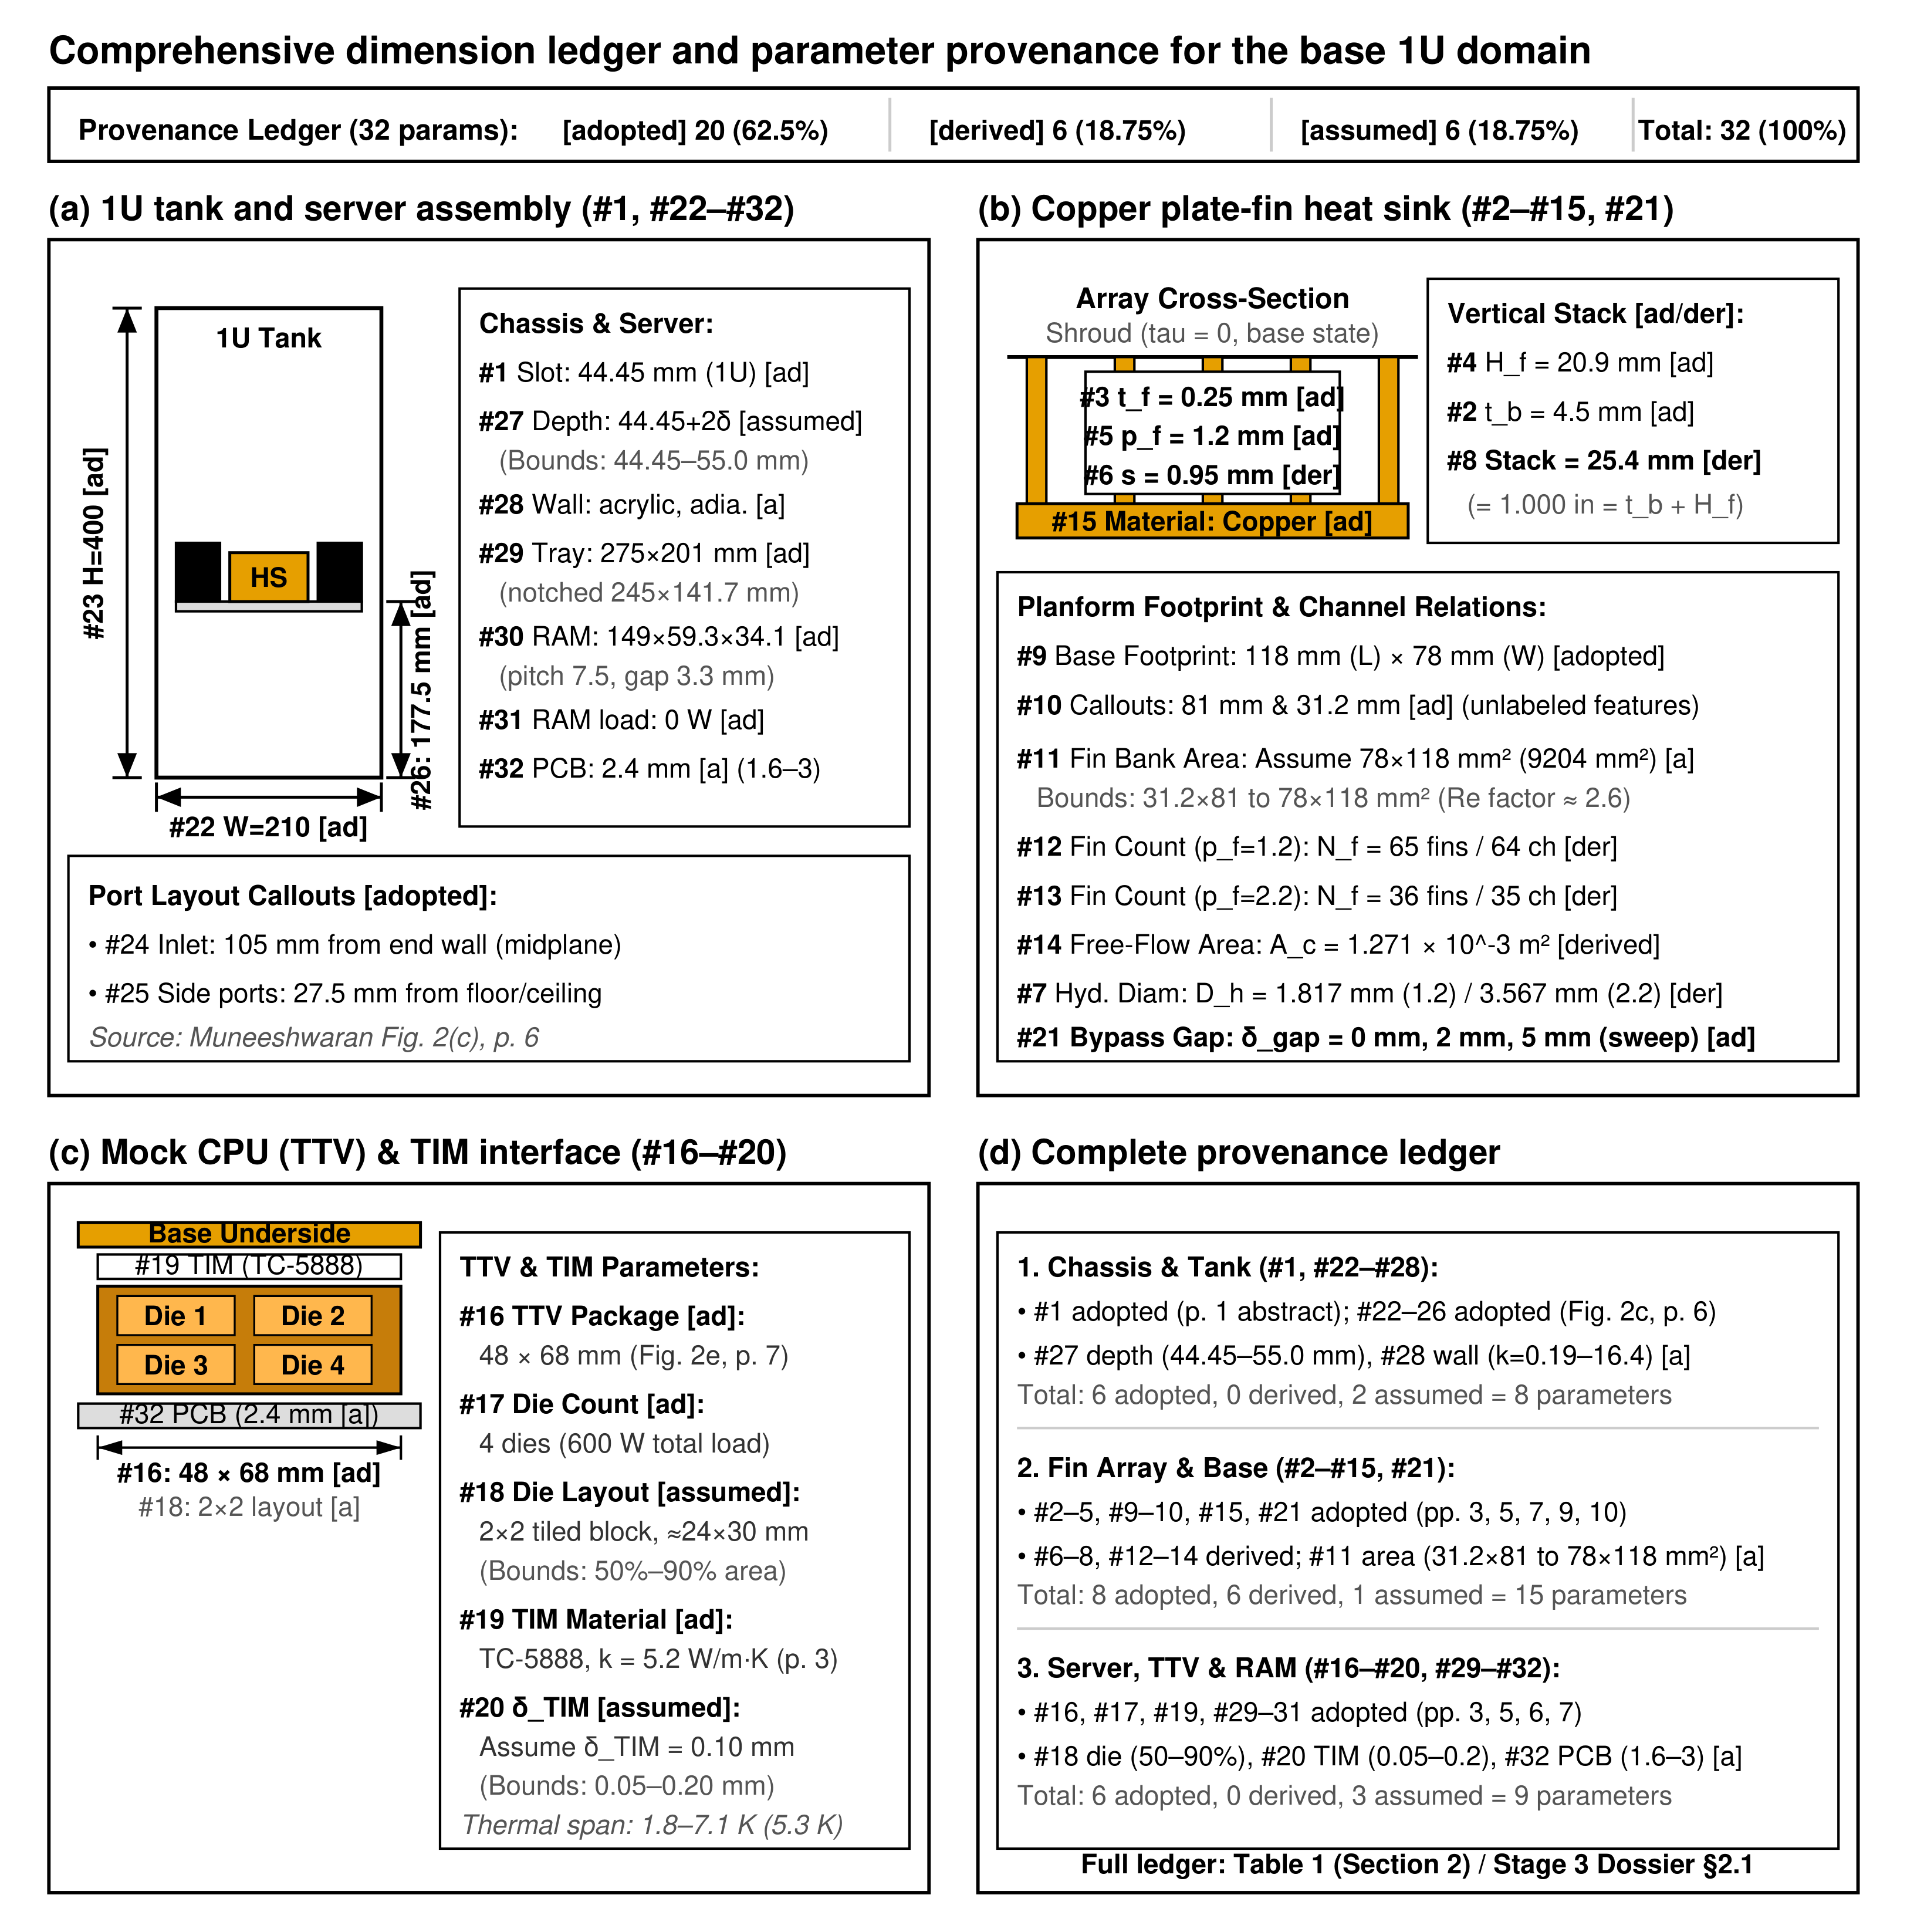
\includegraphics[width=\textwidth]{../figures/fig2_dimension_ledger.png}
\caption{Dimension ledger and parameter provenance for the base model geometry, matching
Table~\ref{tab:ledger-base}. Adopted, derived and assumed dimensions are visually distinguished
so that the source of every number in the model is visible at a glance.}
\label{fig:ledger}
\end{figure}

Two conventions follow from the ledger and are stated here so that no downstream quantity is
ambiguous. First, the fin bank is taken to span the 78~mm base width, so the span sets the channel
count and the 118~mm base length is the channel flow length. Second, the channel hydraulic
diameter of row 7 is the length scale for every Reynolds and Nusselt number reported in this
paper. That second point needs saying because the bypass and tip-clearance literature this work
builds on does not share a convention: Sastre et al.~\cite{sastre2018} use the hydraulic diameter
of the finned cross-section including the clearance slab, Mei et al.~\cite{mei2014} use the pin
diameter with the maximum velocity, Jeng~\cite{jeng2008} uses the bare rectangular duct with the
inlet velocity, Shahsavar et al.~\cite{shahsavar2021} use four times the array volume over its
wetted area, Shrigondekar et al.~\cite{shrigondekar2023} use the bare fin spacing, and Min et
al.~\cite{min2004} report no Reynolds number at all and sweep pumping power instead. Five
incompatible length scales across six papers is a large part of why no dimensionless framework for
this problem exists yet, and every literature value quoted in this paper is recomputed on the
convention above before it is compared with anything.

Applying that convention to the base geometry gives a channel Reynolds number
$\mathrm{Re}_{ch}=\dot{m}D_h/(A_c\mu)$ of roughly 5 to 122 over the 1 to 3~LPM flow range and the
15 to 35~$^{\circ}$C inlet range, if all flow is forced through the fins. The band is wide, and it
is wide for an honest reason: it carries the factor of about 2.6 between the two bounds of the
fin-bank span in row 11. No single-valued channel Reynolds number is quoted for the base geometry
anywhere in this paper. The one directly printed check available is Shrigondekar et
al.~\cite{shrigondekar2023}, who report a fin-spacing Reynolds number of about 10 to 70 for FC-40
on the same rig at the same flow rates and the same two fin pitches. Converted onto the fin-spacing
length scale, the wide-span bound of row 11 gives 2.5 to 46 and the narrow-span bound gives 6.4 to
114. The printed value therefore sits inside the narrow band and partly above the wide one, which
means this check leans against the value adopted rather than confirming it. That is recorded here
rather than smoothed over.

\subsection{Reference configuration for the anchor comparison}
\label{sec:v3}

A second, fully dimensioned geometry is carried alongside the base model so that the open-ratio
results of Chun et al.~\cite{chun2026} can be reproduced without rescaling anything.
Table~\ref{tab:ledger-v3} is its ledger. It is not a substitute for the base model and no result
from the two configurations is pooled.

\begingroup
\footnotesize
\setlength{\tabcolsep}{4pt}
\begin{longtable}{@{}l>{\raggedright\arraybackslash}p{0.225\textwidth}>{\raggedright\arraybackslash}p{0.185\textwidth}l>{\raggedright\arraybackslash}p{0.245\textwidth}@{}}
\caption{Dimension ledger for the reference configuration used in the anchor comparison, the 1U
plate-fin build of Chun et al.~\cite{chun2026}. Page numbers are the printed journal page of
\textit{Energy} \textbf{361} (2026) 141967.}
\label{tab:ledger-v3}\\
\toprule
\# & Quantity & Value & Tag & Source or arithmetic \\
\midrule
\endfirsthead
\multicolumn{5}{@{}l}{\normalfont\itshape Table~\ref{tab:ledger-v3} continued}\\
\toprule
\# & Quantity & Value & Tag & Source or arithmetic \\
\midrule
\endhead
\midrule
\multicolumn{5}{@{}r}{\normalfont\itshape continued on next page}\\
\endfoot
\bottomrule
\endlastfoot
A1  & 1U internal slot spacing        & 44.45~mm & \texttt{[adopted]} & p.~5, \S2.1 \\
A2  & Fin thickness                   & 2~mm     & \texttt{[adopted]} & Fig.~2(a), p.~5, callout under a ``Unit : mm'' header \\
A3  & Fin spacing                     & 3~mm     & \texttt{[adopted]} & Fig.~2(a), p.~5 \\
A4  & Fin height                      & 20~mm    & \texttt{[adopted]} & Fig.~2(a), p.~5 \\
A5  & Fin pitch                       & 5~mm     & \texttt{[derived]} & $2+3$ \\
A6  & Heat-sink base plate            & 72~mm width $\times$ 106~mm flow length & \texttt{[adopted]} & Fig.~2(a), p.~5 \\
A7  & Fin count                       & 15 fins, 14 channels & \texttt{[derived]} & $2N+3(N-1)=72$ gives $N=15$ exactly \\
A8  & Channel free-flow area          & $8.40\times10^{-4}$~m$^2$ & \texttt{[derived]} & $14\times3\times20$~mm$^2$ \\
A9  & Channel hydraulic diameter      & 5.217~mm & \texttt{[derived]} & $2(3)(20)/23$ \\
A10 & Copper block, mock CPU          & 50 $\times$ 65 $\times$ 8~mm & \texttt{[adopted]} & Fig.~2(a), p.~5 \\
A11 & TIM, indium foil thickness      & $\approx$0.1~mm & \texttt{[adopted]} & p.~6, \S2.1 \\
A12 & Heat-sink centre spacing on PCB & 60~mm    & \texttt{[adopted]} & p.~6, \S2.1, and Fig.~2(a), p.~5 \\
A13 & Tank internal width             & 423~mm   & \texttt{[adopted]} & Fig.~2(a), p.~5, right-hand panel headed ``Immersion tank'' \\
A14 & Tank internal height, outlet plane to distribution-plate plane & 430~mm & \texttt{[adopted]} & Fig.~2(a), p.~5, right-hand panel \\
A15 & Distribution plate, 1U build    & 10 holes, 10~mm diameter & \texttt{[adopted]} & p.~5, \S2.1 \\
A16 & Distribution plate, 3U build    & 30 holes, 5~mm diameter & \texttt{[adopted]} & p.~5, \S2.1 \\
A17 & Tank material                   & SUS304, double-layer insulation, tempered-glass window & \texttt{[adopted]} & p.~4, \S2.1; properties Table~2, p.~6 \\
A18 & Flow-control block material     & acrylic  & \texttt{[adopted]} & p.~6, \S2.1 \\
A19 & Flow-control block dimensions   & not dimensioned in the source & \texttt{[assumed]} & The open ratio is therefore defined here by the volume a block occludes, never by a block dimension \\
A20 & Tank external envelope          & not printed in the source & \texttt{[assumed]} & Not required: the computational domain is the wetted interior bounded by A13, A14 and A1 \\
A21 & Metal-foam alternative core     & 10~PPI, porosity 0.9; sweep 5 to 15~PPI, porosity 0.5 to 0.9 & \texttt{[adopted]} & p.~15 and p.~18, \S3.3 \\
\end{longtable}
\endgroup

Three specific gaps in this reference configuration are carried openly rather than closed
silently, because an independent reproducibility check found them and they are real. The source
does not print the tank's third, out-of-plane dimension, does not print the heat-sink base
thickness, and does not give the numerical inlet profile, outlet type or tank-wall thermal
condition, so the anchor comparison in Section~\ref{sec:verification} is a best-effort check
against a paper that does not fully close its own specification, not a fully reproducible
benchmark. The same three gaps are the reason A19, A20 and the base thickness never enter a
reported quantity.

\subsection{Open ratio}
\label{sec:openratio}

The bypass metric is adopted verbatim from Chun et al.~\cite{chun2026}, who introduce it as an
unnumbered display equation on their p.~11 and illustrate it in their Fig.~8. Their words for it,
quoted so that nothing is quietly reinterpreted here, are that the open ratio is
\textit{the volumetric fraction of the unobstructed fluid inlet space relative to the total heat
sink inlet volume}:

\begin{equation}
\mathrm{OR} = \frac{V_{\mathrm{open}}}{V_{\mathrm{total}}}\times 100 \quad (\%)
\label{eq:or}
\end{equation}

\noindent
Named for the geometry of Table~\ref{tab:ledger-base}, the two volumes in Eq.~(\ref{eq:or}) are
the following. $V_{\mathrm{total}}$ is the total heat-sink inlet volume, the fluid volume swept
out by the heat-sink inlet plane over the inlet-plane thickness, that is the plan area of the 1U
slot facing the heat sink multiplied by the inlet-plane thickness, spanning the full tank width
available to the flow at that height. $V_{\mathrm{open}}$ is the unobstructed fluid inlet space,
the part of $V_{\mathrm{total}}$ occupied by neither the heat sink nor a flow-control block, that
is the volume through which fluid can reach the outlets without passing between the fins. At
$\mathrm{OR}=100\%$ the tank is unobstructed and bypass is free. At $\mathrm{OR}=0\%$ every
entering parcel is directed through the heat-source region.

Three properties of the definition travel with it, because dropping any of them changes what the
number means. It is a volume ratio at the inlet plane, not an area ratio and not a clearance in
millimetres; the source never converts it to a gap width. It is geometry-specific, and the source
says so, so any open ratio quoted here travels with the geometry it was measured on. And the
blocking acts laterally, from both edges symmetrically, which in the 1U build means the top gap is
absent and the open ratio is a purely lateral quantity.

Open ratio is a geometric input. Its companion output, also taken from
Chun et al.~\cite{chun2026}, is the bypass mass fraction,

\begin{equation}
\dot{m}_{\mathrm{bypass}} = \dot{m}_{\mathrm{total}} - \dot{m}_{\mathrm{active}},
\qquad
\Phi_{\mathrm{bypass}} = \frac{\dot{m}_{\mathrm{bypass}}}{\dot{m}_{\mathrm{total}}}\times 100
\quad (\%),
\label{eq:phibypass}
\end{equation}

\noindent
where the bypass region is the flow region excluding the heat-sink passages and the region
directed toward the heat source. This paper reports $\mathrm{OR}$ as the design variable and
$\Phi_{\mathrm{bypass}}$ as the computed response, in the same pairing the source uses.

Lateral bypass and tip clearance are carried as two separate parameters and are never combined
into one scalar. The tip clearance ratio is defined as

\begin{equation}
\tau = \frac{c}{H_f},
\label{eq:tau}
\end{equation}

\noindent
the clearance height over the fin height, and is held at $\tau=0$ in the base configuration. Four
reasons keep the two apart. The 1U build that defines the open ratio has already eliminated the
top gap, so folding a tip term into it would redefine the source's own quantity while keeping its
name. No study surveyed here varies both mechanisms; every tip-clearance study varies only the tip
gap and both side-bypass studies vary only the side gap, so a combined ratio would be a quantity
with no supporting measurement anywhere. Jeng~\cite{jeng2008} argues the point directly, noting
that the tip gap dominates in magnitude and can be changed late in a design while the channel
width is fixed early by the board width, which in a 1U immersion chassis holds with extra force.
And the two responses have different shapes. Tip clearance is non-monotonic and has an interior
optimum: Min et al.~\cite{min2004} report a minimum thermal resistance of 0.058~$^{\circ}$C~W$^{-1}$
at a clearance-to-channel-width ratio of 0.6 under 2.27~W of pumping power, and Mei et
al.~\cite{mei2014} report the same competing-effects reversal. Lateral bypass is monotonic and
always detrimental, in Muneeshwaran et al.~\cite{muneeshwaran2023} across the 0 to 5~mm gap sweep
and in Chun et al.~\cite{chun2026} across the open-ratio sweep. Collapsing a bounded parameter
with an optimum and a monotone detrimental one into a single scalar would make any interior
optimum in the combined ratio unattributable to either mechanism. Sastre et al.~\cite{sastre2018}
supply the warning empirically: even one clearance parameter was strong enough to split their
Nusselt-Graetz curves into separate families rather than one fit.

One out-of-sample check on the open ratio exists and is used. Jeng~\cite{jeng2008} parameterises
lateral bypass around a square pin-fin sink as the ratio $W/L$ of channel width to sink length. For
a constant-height inlet plane the two parameterisations map exactly, $\mathrm{OR} = (1-L/W)\times
100$, so $W/L$ of 1, 2, 3 and 5 correspond to open ratios of 0, 50, 66.7 and 80\%. Jeng's
recommendation of $W/L$ between 2 and 3 therefore sits inside the range swept here, in a different
fluid and a different fin type. The mapping is derived here, not printed in either source, and it
holds only when the open volume is the lateral space at the same inlet-plane height.

\subsection{Working fluids and thermophysical properties}
\label{sec:properties}

Two dielectric coolants are used. FC-40, a perfluorinated fluorocarbon, is the primary fluid: it is
the one coolant for which more than one independent group in this literature has published usable
property data, so a property error can be caught by cross-checking rather than trusted. GC-5X, an
oil-based dielectric, is the high-viscosity contrast case. Carrying two fluids is not decoration.
Chun et al.~\cite{chun2026} show that open-ratio sensitivity is a strong function of viscosity,
with thermal resistance falling 6.1\% for FC-40 but 45.6\% for GC-5X as the bypass is closed, so a
framework claimed to be dimensionless must be exercised across more than one Prandtl decade or the
claim is untested.

Table~\ref{tab:fluidprops} gives the property treatment and the source of every value.

\begin{table}[htbp]
\centering
\caption{Coolant thermophysical properties and their sources. The correlations of Chun et
al.~\cite{chun2026} take $T$ in kelvin; see the discussion below.}
\label{tab:fluidprops}
\footnotesize
\setlength{\tabcolsep}{4pt}
\begin{tabular}{@{}l>{\raggedright\arraybackslash}p{0.105\textwidth}>{\raggedright\arraybackslash}p{0.405\textwidth}>{\raggedright\arraybackslash}p{0.215\textwidth}@{}}
\toprule
Fluid & Property & Value or correlation ($T$ in K) & Source \\
\midrule
FC-40 & $\rho$    & $2499 - 2.16\,T$~kg~m$^{-3}$ & \cite{chun2026}, Table~3, p.~7 \\
FC-40 & $k$       & $0.086 - 6.90\times10^{-5}\,T$~W~m$^{-1}$~K$^{-1}$ & \cite{chun2026}, Table~3, p.~7 \\
FC-40 & $c_p$     & $590 + 1.55\,T$~J~kg$^{-1}$~K$^{-1}$ & \cite{chun2026}, Table~3, p.~7 \\
FC-40 & $\mu$     & $0.0429 - 0.162\times10^{-3}\,T$ $+\;1.08\times10^{-7}\,T^2$~Pa~s & \cite{chun2026}, Table~3, p.~7 \\
FC-40 & $\rho$ & 1874.44~kg~m$^{-3}$ at 16~$^{\circ}$C & \cite{muneeshwaran2023}, Table~4, p.~7 \\
FC-40 & $\nu$ & $5\times10^{-6}$, $1.5\times10^{-6}$, $5.4\times10^{-7}$~m$^2$~s$^{-1}$ at 0, 40, 100~$^{\circ}$C & \cite{muneeshwaran2023}, Table~4, p.~7 \\
FC-40 & $c_p$ & 1014, 1076, 1169.4~J~kg$^{-1}$~K$^{-1}$ at 0, 40, 100~$^{\circ}$C & \cite{muneeshwaran2023}, Table~4, p.~7 \\
FC-40 & $k$ & 0.067, 0.0642, 0.0601~W~m$^{-1}$~K$^{-1}$ at 0, 40, 100~$^{\circ}$C & \cite{muneeshwaran2023}, Table~4, p.~7 \\
FC-40 & $\beta$   & $1.2\times10^{-3}$~K$^{-1}$ & \cite{muneeshwaran2023}, Table~4, p.~7 \\
FC-40 & Boiling pt. & 165~$^{\circ}$C at 1~bar & \cite{muneeshwaran2023}, Table~4, p.~7 \\
FC-40 & $\mathrm{Pr}$ & 67.5 at 25~$^{\circ}$C & \texttt{[derived]} from the correlations above \\
\midrule
GC-5X & $\rho$    & $1049.862 - 0.75\,T$~kg~m$^{-3}$ & \cite{chun2026}, Table~3, p.~7 \\
GC-5X & $k$       & $0.199367 - 1.8\times10^{-4}\,T$~W~m$^{-1}$~K$^{-1}$ & \cite{chun2026}, Table~3, p.~7 \\
GC-5X & $c_p$     & $2076.055 + 0.3\,T$~J~kg$^{-1}$~K$^{-1}$ & \cite{chun2026}, Table~3, p.~7 \\
GC-5X & $\mu$     & $0.6449 - 4.1234\times10^{-3}\,T$ $+\;8.9697\times10^{-6}\,T^2$ $-\;6.5833\times10^{-9}\,T^3$~Pa~s & \cite{chun2026}, Table~3, p.~7 \\
GC-5X & $\beta$   & $9.08\times10^{-4}$~K$^{-1}$ at 25~$^{\circ}$C & \texttt{[derived]}, $\beta=-\rho^{-1}\partial\rho/\partial T$ on the density fit of this table. No measured value is printed in any source consulted \\
GC-5X & $\mathrm{Pr}$ & 570 at 25~$^{\circ}$C & \texttt{[derived]} from the correlations above \\
\bottomrule
\end{tabular}
\end{table}

Two findings about these properties came out of checking them rather than copying them, and both
change how the correlations may be used.

The first is that the correlations of Chun et al.~\cite{chun2026} take $T$ in kelvin, which their
paper does not state and their own nomenclature contradicts by defining $T$ in degrees Celsius.
The evidence is arithmetic and it is decisive. With $T$ in kelvin the FC-40 density fit returns
1874.4~kg~m$^{-3}$ at 289.15~K, against the 1874.44~kg~m$^{-3}$ at 16~$^{\circ}$C measured
independently by Muneeshwaran et al.~\cite{muneeshwaran2023}. The conductivity fit returns 0.0672,
0.0644 and 0.0603~W~m$^{-1}$~K$^{-1}$ at 0, 40 and 100~$^{\circ}$C against their printed 0.067,
0.0642 and 0.0601, and the specific-heat fit returns 1013.4, 1075.4 and 1168.4~J~kg$^{-1}$~K$^{-1}$
against their printed 1014, 1076 and 1169.4. Three properties agree to better than 0.1\% at three
temperatures each on one unit convention and are irreconcilable on the other. The same conclusion
follows independently from the source's own mass-flow table, which converts to exactly 5.00~LPM per
heat sink at the stated 10~LPM for two heat sinks only when the density is evaluated in kelvin.
This is an inference from the paper's numbers, not a printed statement, and it should be confirmed
with the corresponding author before any anchor result is reproduced.

The second finding is a limit on the FC-40 viscosity fit, and it constrains the model. That
quadratic reaches zero at about 343~K, or 70~$^{\circ}$C, and is negative above it, so it cannot be
used at wall temperatures approaching the 80~$^{\circ}$C case-temperature limit of the base
paper~\cite{muneeshwaran2023}. Within its useful band it is good: against the kinematic-viscosity
points of Muneeshwaran et al.\ interpolated logarithmically it agrees to 1.2\% at 35~$^{\circ}$C
and 3.9\% at 25~$^{\circ}$C, degrading to 13\% at 15~$^{\circ}$C and 30\% at 0~$^{\circ}$C. FC-40
viscosity is therefore evaluated from the fit between 20 and 60~$^{\circ}$C and from the measured
points of Muneeshwaran et al.\ outside that band. The GC-5X cubic stays positive and monotone
across the whole range of interest and needs no such restriction.

Solid properties are listed in Table~\ref{tab:solidprops}. Where two sources print a value, both
are named, and where they agree exactly that is said, because agreement between independently
published tables is the only property check available in the absence of a measurement of our own.

\begin{table}[htbp]
\centering
\caption{Solid domain properties and their sources. Density in kg~m$^{-3}$, specific heat in J~kg$^{-1}$~K$^{-1}$, thermal conductivity in W~m$^{-1}$~K$^{-1}$.}
\label{tab:solidprops}
\footnotesize
\setlength{\tabcolsep}{4pt}
\begin{tabular}{@{}>{\raggedright\arraybackslash}p{0.155\textwidth}cc>{\raggedright\arraybackslash}p{0.105\textwidth}>{\raggedright\arraybackslash}p{0.30\textwidth}@{}}
\toprule
Domain & $\rho$ & $c_p$ & $k$ & Source \\
\midrule
Copper, fins and base & 8978 & 381 & 387.6 & \cite{chun2026}, Table~2, p.~6; the identical triplet is printed independently in \cite{khoshvaghtaliabadi2026oblique}, Table~1, p.~5 \\
TIM, base model, thermal grease & \multicolumn{2}{c}{not printed} & 5.2 & \cite{muneeshwaran2023}, p.~3, \S2.1 \\
TIM, reference configuration, indium & 7310 & 234 & 81.8 & \cite{chun2026}, Table~2, p.~6 \\
PCB substrate & 1850 & 1000 & 0.3 & \cite{khoshvaghtaliabadi2026oblique}, Table~1, p.~5 \\
PCB substrate, alternative & 3600 & 720 & 42.0 in-plane, 0.5 cross-plane & \cite{chun2026}, Table~2, p.~6 \\
SUS304, reference configuration tank & 8000 & 500 & 16.4 & \cite{chun2026}, Table~2, p.~6 \\
Acrylic, flow-control block and tank wall & 1180 & 1460 & 0.21 & \cite{chun2026}, Table~2, p.~6 \\
\bottomrule
\end{tabular}
\end{table}

The two PCB entries disagree by two orders of magnitude in conductivity because they describe
different things: one is an isotropic bulk laminate value, the other resolves the copper-plane
anisotropy. The isotropic entry is used for the base model, where the board is an unloaded
conduction path, and the anisotropic entry is used for the anchor comparison so that the
reference configuration keeps its own source's convention. Neither value moves a reported quantity
in this work, since the board carries no thermal load in the base model. All solid property values
in Table~\ref{tab:solidprops} are attributed within their source to further references rather than
measured there, and are carried on that basis.

\subsection{Assumptions}
\label{sec:assumptions}

Eight quantities in Tables~\ref{tab:ledger-base} and \ref{tab:ledger-v3} are not available in any
source consulted. Each is listed below with the value taken, the reason, the defensible bounds and
the results it can move. Nothing here is assumed because it was convenient, and nothing that a
result depends on is hidden inside a sentence.

\noindent\textbf{Fin-bank plan area, 78~mm $\times$ 118~mm (row 11).}\ The base outline of the heat sink is
dimensioned but the drawing does not label which feature its two interior callouts, 81~mm and
31.2~mm, terminate on. Bounds are therefore 31.2 $\times$ 81~mm at the low end and 78 $\times$
118~mm at the high end, a factor of 3.6 in plan area. The wide value is taken because it is the
only one under which the 48 $\times$ 68~mm mock-processor footprint of row 16 is fully covered by
the fin array. The counter-evidence is stated in Section~\ref{sec:geometry} and is not resolved:
converting the printed fin-spacing Reynolds range of Shrigondekar et al.~\cite{shrigondekar2023}
onto this geometry leans toward the narrow bound. Results moved: the span sets the channel count,
64 channels at 78~mm against 25 at 31.2~mm, hence a free-flow area of 1271~mm$^2$ against
496~mm$^2$, a factor of about 2.6 on channel velocity and on channel Reynolds number. Every
Reynolds number quoted for the base model carries that factor as a band. Thermal resistance is far
less sensitive, since the area enters through fin efficiency and total wetted area rather than
linearly. This is the largest single geometric uncertainty in the model, and the cheapest way to
settle it is a higher-resolution copy of the source drawing or a question to its corresponding
author.

\noindent\textbf{Die partition inside the mock-processor package (row 18).}\ The four dies are drawn as a
tiled block but the block is not dimensioned. Bounds are a die block between 50\% and 90\% of the
48 $\times$ 68~mm package footprint. The assumption is low-risk because the heat load is applied as
a boundary condition at the heat-sink base, following the base paper's own numerical
treatment~\cite{muneeshwaran2023}, so the die partition never enters the model. Results moved: only
a local peak junction temperature post-process, which this paper does not report.

\noindent\textbf{TIM bond-line thickness, 0.10~mm (row 20).}\ The base paper names the grease and gives its
conductivity but not the bond line. The value is set to match the indium-foil thickness printed for
the reference configuration~\cite{chun2026} so that both configurations share one interface
convention. Bounds 0.05 to 0.20~mm, the usual range for a screwed-down grease line. Results moved:
absolute case temperature shifts by about 5.3~K across those bounds ($-1.8$~K to $+3.5$~K relative to
the 0.10~mm nominal) at 600~W over the row 16 footprint. Thermal-resistance differences between open
ratios are insensitive to it, because it is a series resistance common to every case.

\noindent\textbf{Tank depth, 44.45~mm internal plus twice the bypass gap (row 27).}\ Genuinely absent. The tank
drawing carries no callout for the out-of-plane thickness and the body text gives none. The value
is chosen so that the tank interior is exactly the 1U slot the source's own abstract specifies.
Bounds 44.45 to 55~mm internal. Results moved: this dimension sets the bypass area and therefore
is the open ratio. It is the most consequential assumption in the ledger, and it is precisely why
this paper parameterises on the dimensionless open ratio rather than on an absolute tank depth.

\noindent\textbf{Tank wall material and outer boundary (row 28).}\ The base paper never names the tank material.
Acrylic with $k = 0.19$~W~m$^{-1}$~K$^{-1}$ is taken, consistent with the transparent wall in the
source's own photograph, with an adiabatic outer face. Bounds on $k$ run from 0.19 for acrylic to
16.4~W~m$^{-1}$~K$^{-1}$ for the stainless steel used in the reference
configuration~\cite{chun2026}. Results moved: none of those reported. The adiabatic outer face is
the source's own stated condition, since it reports that the entire experimental system was
insulated and that the heat loss was negligible~\cite{muneeshwaran2023}.

\noindent\textbf{PCB thickness, 2.4~mm (row 32).}\ Not given by the base paper. Taken from the only printed
PCB thickness available for a 1U immersion server~\cite{khoshvaghtaliabadi2026oblique}. Bounds 1.6
to 3.0~mm. Results moved: none reported here; the board is an unloaded conduction path of
$k \approx 0.3$~W~m$^{-1}$~K$^{-1}$.

\noindent\textbf{Flow-control block dimensions in the reference configuration (row A19).}\ The blocks are shown
schematically in the source but given no size. The open ratio is therefore defined by the volume a
block occludes, as in Eq.~(\ref{eq:or}), never by a block dimension. Results moved: the mapping
from open ratio to bypass fraction. Since this paper reports the open ratio as an input and the
bypass fraction as a computed output, no reported quantity requires the block geometry.

\noindent\textbf{External tank envelope in the reference configuration (row A20).}\ Not printed. Not required,
because the computational domain is the wetted interior bounded by rows A13, A14 and A1.

A separate set of quantities is held fixed rather than assumed, and each is fixed for a stated
reason. The rack unit height is held at 44.45~mm because it is an industry dimensional standard
printed identically by three independent groups~\cite{muneeshwaran2023,chun2026,kim2025}; it is not
a free design variable, and Kim et al.\ already swept it from 0.8U to 1.2U if a sensitivity
precedent is wanted. The mock-processor footprint is held at 48 $\times$ 68~mm because fixing the
heat-source footprint is what makes the open ratio the only varying geometric quantity; if the
footprint moved, a change in thermal resistance could not be attributed to bypass. The heat-sink
base thickness is held at 4.5~mm because it sets spreading resistance, which sits in series with
the convective resistance the open ratio acts on, so holding it keeps the two separable. The fin
material is held at copper: with a solid-to-fluid conductivity ratio near 6000 for FC-40, fin
efficiency is near unity and the result is insensitive to the copper grade, whereas switching to
aluminium would change fin efficiency and confound the bypass conclusion. The port arrangement is
held at the T-configuration because the base paper shows it is a first-order effect, 12.6\% in
thermal resistance against the Z-configuration, and because under the Z-configuration most of the
fluid bypasses the heat sink anyway; holding it removes a competing bypass mechanism so that the
open ratio is the only one varied~\cite{muneeshwaran2023}.

Fin pitch is deliberately not held constant. It is a second factor at the two printed levels of
1.2 and 2.2~mm, because the pitch and bypass interact: the penalty for opening the gap from 0 to
5~mm is 3\% at the coarse pitch but 7.4\% at the fine one~\cite{muneeshwaran2023}. The coolant is
deliberately not held constant either, for the Prandtl-range reason given in
Section~\ref{sec:properties}.
.
%
% PACKAGES REQUIRED IN main.tex PREAMBLE (not currently present):
%   \usepackage{booktabs}
%   \usepackage{array}      (for the >{\raggedright\arraybackslash}p{} column type)
% =============================================================================

\section{Problem formulation}
\label{sec:formulation}

\subsection{Base geometry}
\label{sec:geometry}

The model geometry is the 1U immersion server of Muneeshwaran et al.~\cite{muneeshwaran2023}:
a copper plate-fin heat sink clamped to a four-die thermal test vehicle on a printed circuit
board, with a bank of non-dissipating memory modules alongside it, the whole tray submerged in a
sealed 1U tank. Coolant enters through a port on the tank floor directly beneath the heat sink
and leaves through two ports at the top of the opposite faces, the arrangement those authors call
the T-configuration. That choice of base is not a matter of taste. It is the only 1U immersion
architecture in the surveyed literature whose server tray, heat sink, tank, memory bank and mock
processor all carry printed dimension callouts, so the domain can be rebuilt without scaling
anything off a figure. It is also the architecture that Chun et al.~\cite{chun2026} identify as
prior bypass-control work, that B. Zhang et al.~\cite{zhang2026} state they reconstructed as their
own computational domain, that Khoshvaght-Aliabadi and co-workers rebuilt twice as a validation
replica~\cite{khoshvaghtaliabadi2026oblique,khoshvaghtaliabadi2026component}, and from which Kim
et al.~\cite{kim2025} took their inlet and outlet arrangement. Only the first of those four is a
reuse of the architecture as a study domain; the others are weaker forms of reliance and are
described here as such.

The bypass mechanism this paper is about is present in the base paper and was measured there.
Muneeshwaran et al.~\cite{muneeshwaran2023} swept the clearance between the heat sink and the 1U
tank inner wall at 5, 2 and 0~mm, reported a 3\% to 7.4\% rise in thermal resistance and a
0.7~$^{\circ}$C to 1.5~$^{\circ}$C rise in case temperature as the gap opened, and adopted the
no-gap build for everything that followed. Their flow visualisation shows the reason: fluid takes
the clearance because its hydraulic resistance is lower, and that stream does no useful heat
transfer. The open ratio of Section~\ref{sec:openratio} is the dimensionless generalisation of
exactly this clearance.

\begin{figure}[htbp]
\centering
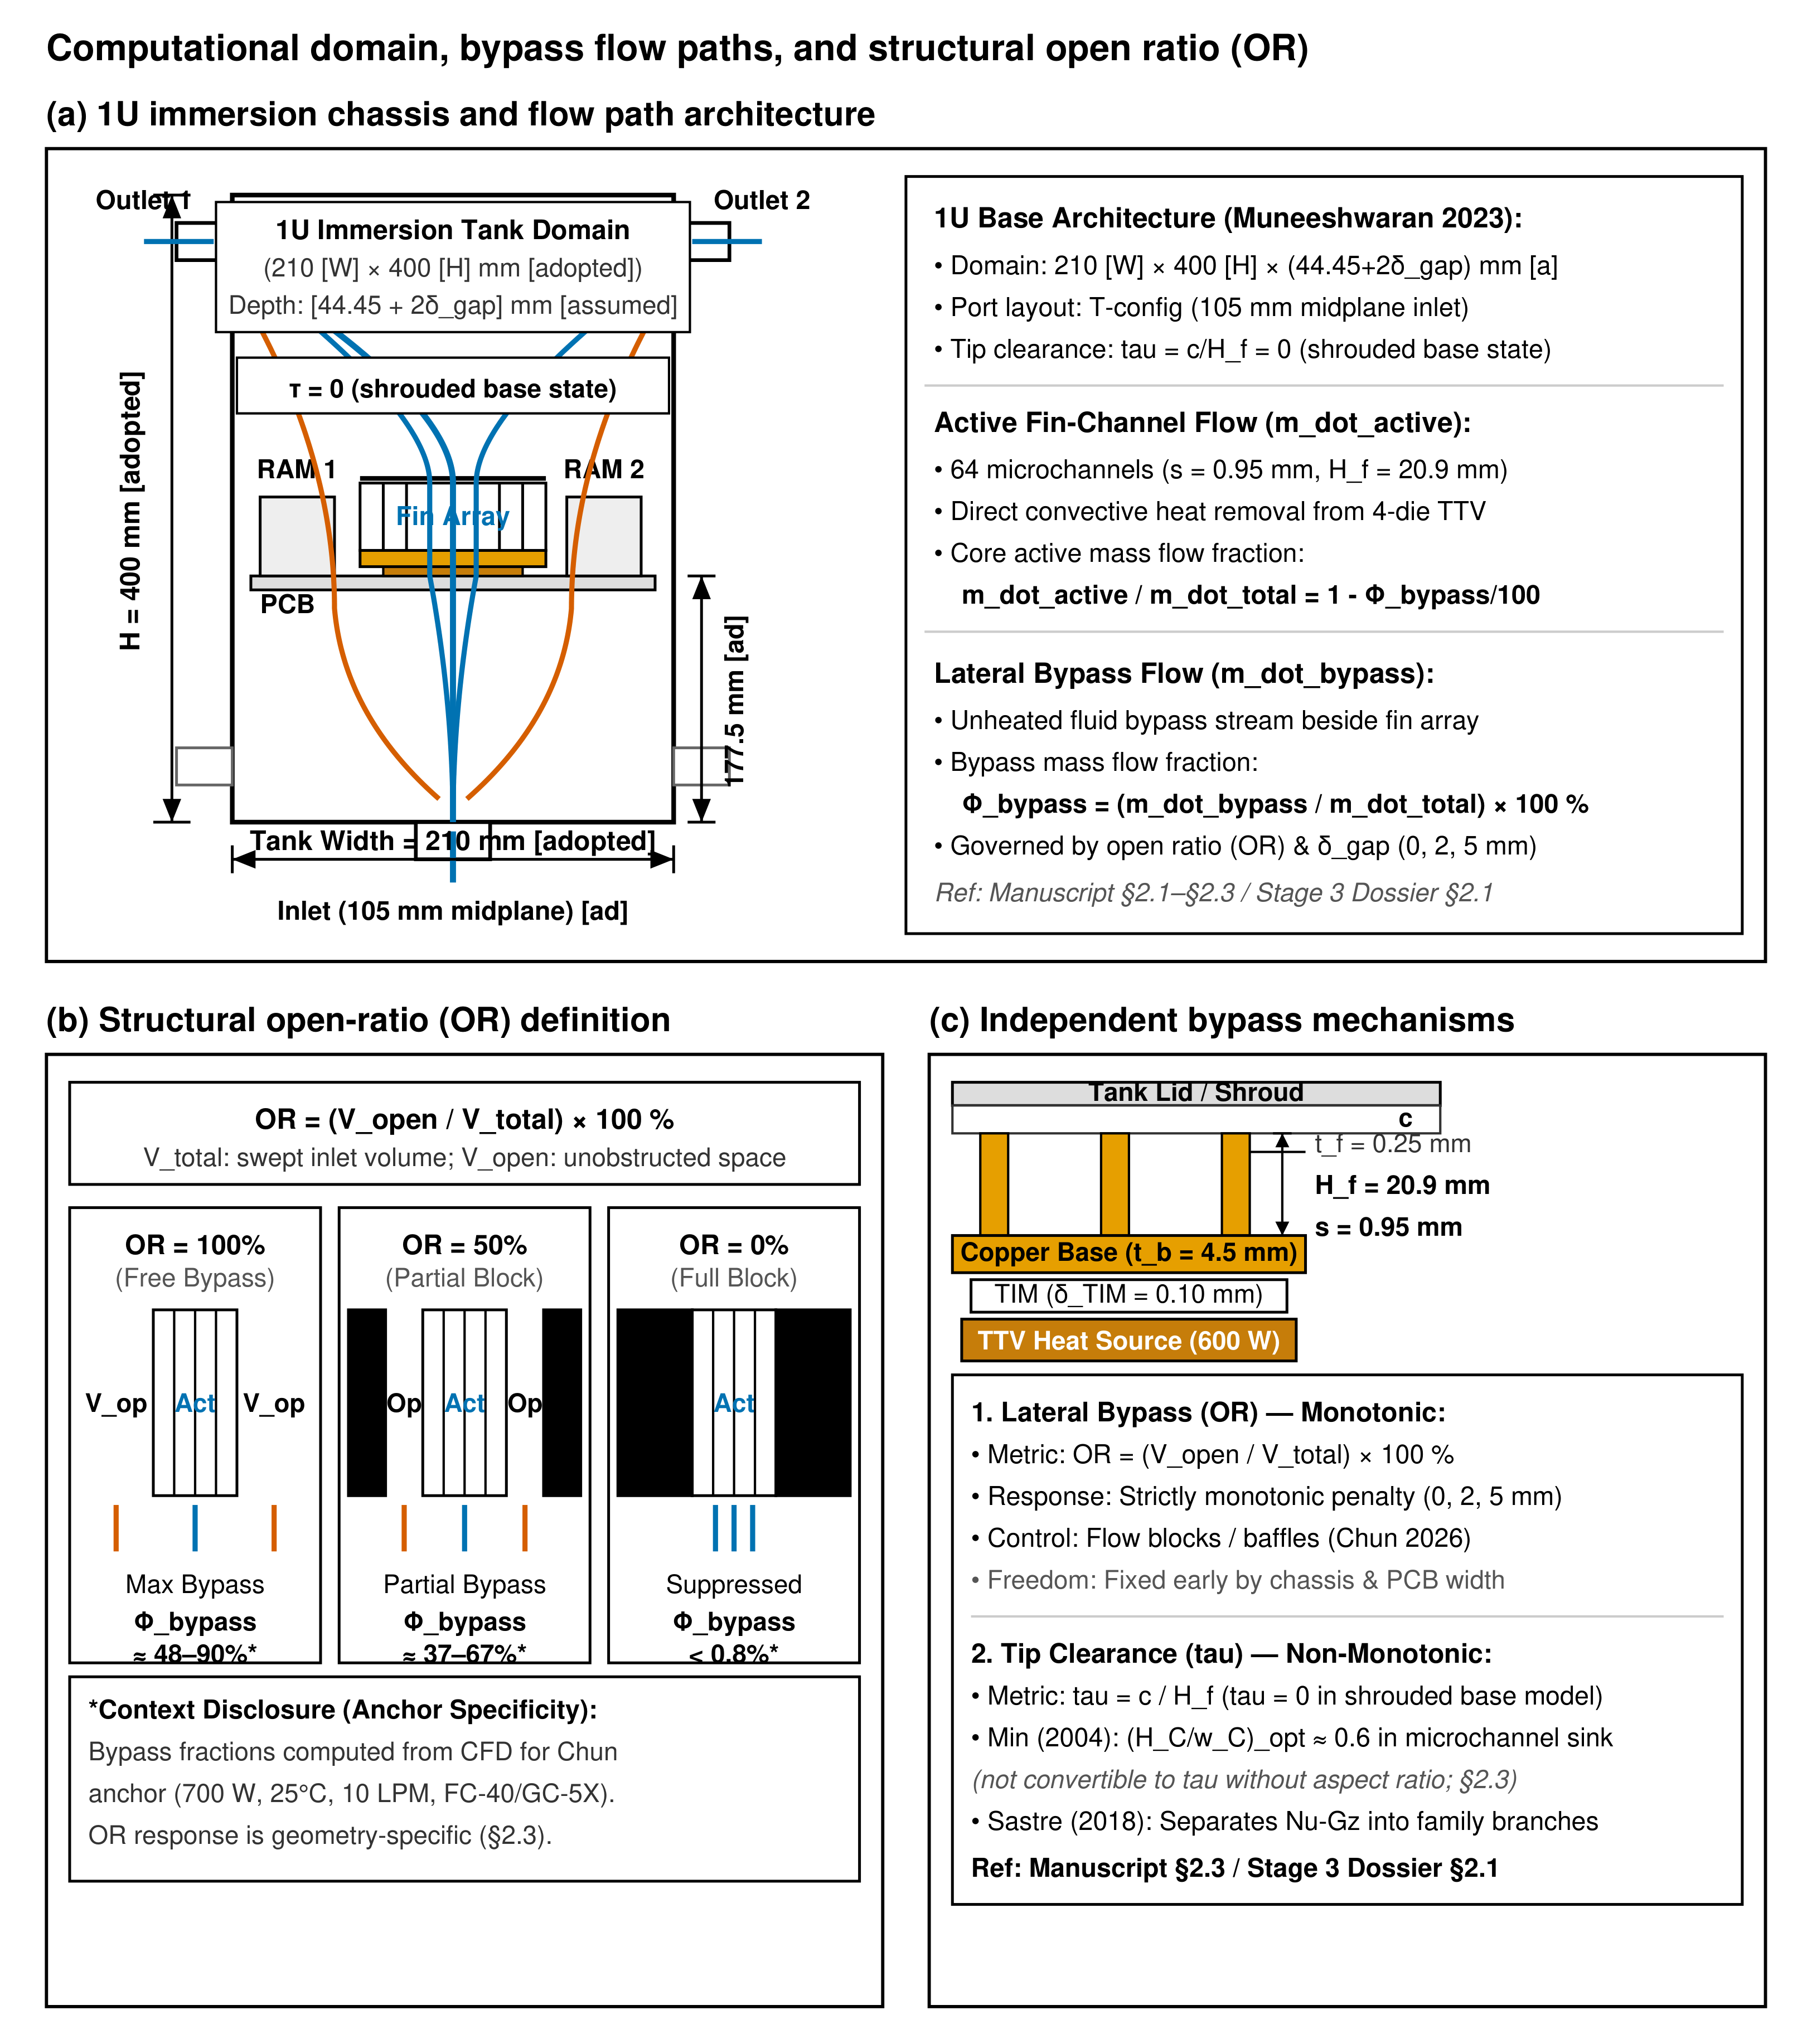
\includegraphics[width=\textwidth]{../figures/fig1_domain.png}
\caption{Computational domain, bypass flow paths and the open-ratio definition. (a) the 1U
immersion chassis with the active fin-channel flow and lateral bypass stream (with the shrouded
$\tau=0$ base state and independent tip clearance treated in panel (c)). (b) the open-ratio
definition at the heat-sink inlet plane across three blockage states. (c) lateral bypass and tip
clearance shown as the two independent mechanisms carried separately in this model, per
Section~\ref{sec:openratio}.}
\label{fig:domain}
\end{figure}

Table~\ref{tab:ledger-base} is the complete dimension ledger for the base model. Every row carries
one of three tags. A row tagged \texttt{[adopted]} is printed in the cited source at the cited
page, in body text, in a table, or as a dimension callout drawn on a figure. A row tagged
\texttt{[derived]} is computed from \texttt{[adopted]} rows, with the arithmetic shown. A row
tagged \texttt{[assumed]} is not available in any source consulted, and its value, its bounds and
the results it can move are stated in Section~\ref{sec:assumptions}. No row in the ledger is
digitised from a plot. Several of the \texttt{[adopted]} rows are recoverable only by rendering
the source page to an image and reading the drawing, because plain text extraction drops
dimension callouts that exist as vector labels inside a figure; those rows name the figure.

\begingroup
\footnotesize
\setlength{\tabcolsep}{4pt}
\begin{longtable}{@{}r>{\raggedright\arraybackslash}p{0.200\textwidth}c>{\raggedright\arraybackslash}p{0.135\textwidth}l>{\raggedright\arraybackslash}p{0.275\textwidth}@{}}
\caption{Dimension ledger for the base model, the 1U immersion server of Muneeshwaran et
al.~\cite{muneeshwaran2023}. Page numbers are the printed journal page of
\textit{Int.\ Commun.\ Heat Mass Transf.} \textbf{145} (2023) 106843, which coincides with the
PDF page index for this article.}
\label{tab:ledger-base}\\
\toprule
\# & Quantity & Symbol & Value & Tag & Source or arithmetic \\
\midrule
\endfirsthead
\multicolumn{6}{@{}l}{\normalfont\itshape Table~\ref{tab:ledger-base} continued}\\
\toprule
\# & Quantity & Symbol & Value & Tag & Source or arithmetic \\
\midrule
\endhead
\midrule
\multicolumn{6}{@{}r}{\normalfont\itshape continued on next page}\\
\endfoot
\bottomrule
\endlastfoot
1  & Rack unit height, server slot        &            & 44.45~mm & \texttt{[adopted]} & p.~1, abstract \\
2  & Heat-sink base thickness             & $t_b$      & 4.5~mm   & \texttt{[adopted]} & p.~3, \S2.1 \\
3  & Fin thickness                        & $t_f$      & 0.25~mm  & \texttt{[adopted]} & p.~3, \S2.1 \\
4  & Fin height                           & $H_f$      & 20.9~mm  & \texttt{[adopted]} & p.~3, \S2.1 \\
5  & Fin pitch, two builds                & $p_f$      & 1.2 and 2.2~mm & \texttt{[adopted]} & p.~3; Table~3, p.~7 \\
6  & Fin channel width                    & $s$        & 0.95~mm; 1.95~mm & \texttt{[derived]} & $s=p_f-t_f$ \\
7  & Channel hydraulic diameter           & $D_h$      & 1.817~mm; 3.567~mm & \texttt{[derived]} & $D_h=2sH_f/(s+H_f)$ \\
8  & Heat-sink stack height               & $t_b+H_f$  & 25.4~mm  & \texttt{[derived]} & $4.5+20.9$ \\
9  & Heat-sink base footprint             & $L\times W$& 118~mm $\times$ 78~mm & \texttt{[adopted]} & Fig.~2(b), p.~5, rendered callouts \\
10 & Raised finned-section callouts       &            & 81~mm and 31.2~mm & \texttt{[adopted]} & Fig.~2(b), p.~5. The drawing does not label which feature each callout terminates on \\
11 & Fin-bank plan area                   & $A_{bank}$ & 78~mm $\times$ 118~mm & \texttt{[assumed]} & Bounds 31.2 $\times$ 81~mm to 78 $\times$ 118~mm; see Section~\ref{sec:assumptions} \\
12 & Fin count, $p_f=1.2$~mm              & $N_f$      & 65 fins, 64 channels & \texttt{[derived]} & $Nt_f+(N-1)s=W$ on row 11 \\
13 & Fin count, $p_f=2.2$~mm              & $N_f$      & 36 fins, 35 channels & \texttt{[derived]} & same relation on row 11 \\
14 & Channel free-flow area, base build   & $A_c$      & $1.271\times10^{-3}$~m$^2$ & \texttt{[derived]} & $64\times0.95\times20.9$~mm$^2$ \\
15 & Heat-sink material                   &            & copper   & \texttt{[adopted]} & p.~3, \S2.1 \\
16 & Mock CPU package footprint           &            & 48~mm $\times$ 68~mm & \texttt{[adopted]} & Fig.~2(e), p.~7, rendered callouts \\
17 & Die count                            &            & 4, independently modulated & \texttt{[adopted]} & p.~3, \S2.1; Fig.~2(e), p.~7 \\
18 & Individual die footprint             &            & 2 $\times$ 2 tiling of a centred block & \texttt{[assumed]} & Bounds 50\% to 90\% of the package footprint; see Section~\ref{sec:assumptions} \\
19 & Thermal interface material           &            & grease TC-5888, $k=5.2$ &  \texttt{[adopted]} & p.~3, \S2.1; $k$ in W~m$^{-1}$~K$^{-1}$ \\
20 & TIM bond-line thickness              & $\delta_{TIM}$ & 0.10~mm & \texttt{[assumed]} & Bounds 0.05 to 0.20~mm; see Section~\ref{sec:assumptions} \\
21 & Bypass gap, heat sink to tank wall   & $\delta_{gap}$ & 0, 2, 5~mm & \texttt{[adopted]} & p.~5, \S3.2; Fig.~6, p.~9; Fig.~7, p.~10 \\
22 & Tank, long horizontal dimension      &            & 210~mm   & \texttt{[adopted]} & Fig.~2(c), p.~6, rendered callouts \\
23 & Tank, vertical dimension             &            & 400~mm   & \texttt{[adopted]} & Fig.~2(c), p.~6 \\
24 & Bottom inlet axis from tank end wall &            & 105~mm   & \texttt{[adopted]} & Fig.~2(c), p.~6; $105=210/2$, so the inlet is on the tank mid-plane \\
25 & Side port axes from floor and ceiling&            & 27.5~mm  & \texttt{[adopted]} & Fig.~2(c), p.~6 \\
26 & Heat-sink underside above tank floor &            & 177.5~mm & \texttt{[adopted]} & Fig.~2(c), p.~6 \\
27 & Tank depth, out-of-plane             &            & 44.45~mm internal $+\,2\delta_{gap}$ & \texttt{[assumed]} & Bounds 44.45 to 55~mm internal; see Section~\ref{sec:assumptions} \\
28 & Tank wall material                   &            & acrylic, adiabatic outer face & \texttt{[assumed]} & $k=0.19$; bounds 0.19 to 16.4~W~m$^{-1}$~K$^{-1}$; see Section~\ref{sec:assumptions} \\
29 & Server tray outline                  &            & 275 and 245~mm; 201 and 141.7~mm & \texttt{[adopted]} & Fig.~2(a), p.~5, rendered callouts \\
30 & Memory bank envelope                 &            & 149 $\times$ 59.3 $\times$ 34.1~mm; pitch 7.5~mm; gap 3.3~mm & \texttt{[adopted]} & Fig.~2(d), p.~6, rendered callouts \\
31 & Memory thermal load                  &            & zero, flow obstruction only & \texttt{[adopted]} & p.~3, \S2.1 \\
32 & PCB thickness                        &            & 2.4~mm   & \texttt{[assumed]} & From Khoshvaght-Aliabadi et al.~\cite{khoshvaghtaliabadi2026oblique}, Table~1, p.~5; bounds 1.6 to 3.0~mm \\
\end{longtable}
\endgroup

\begin{figure}[htbp]
\centering
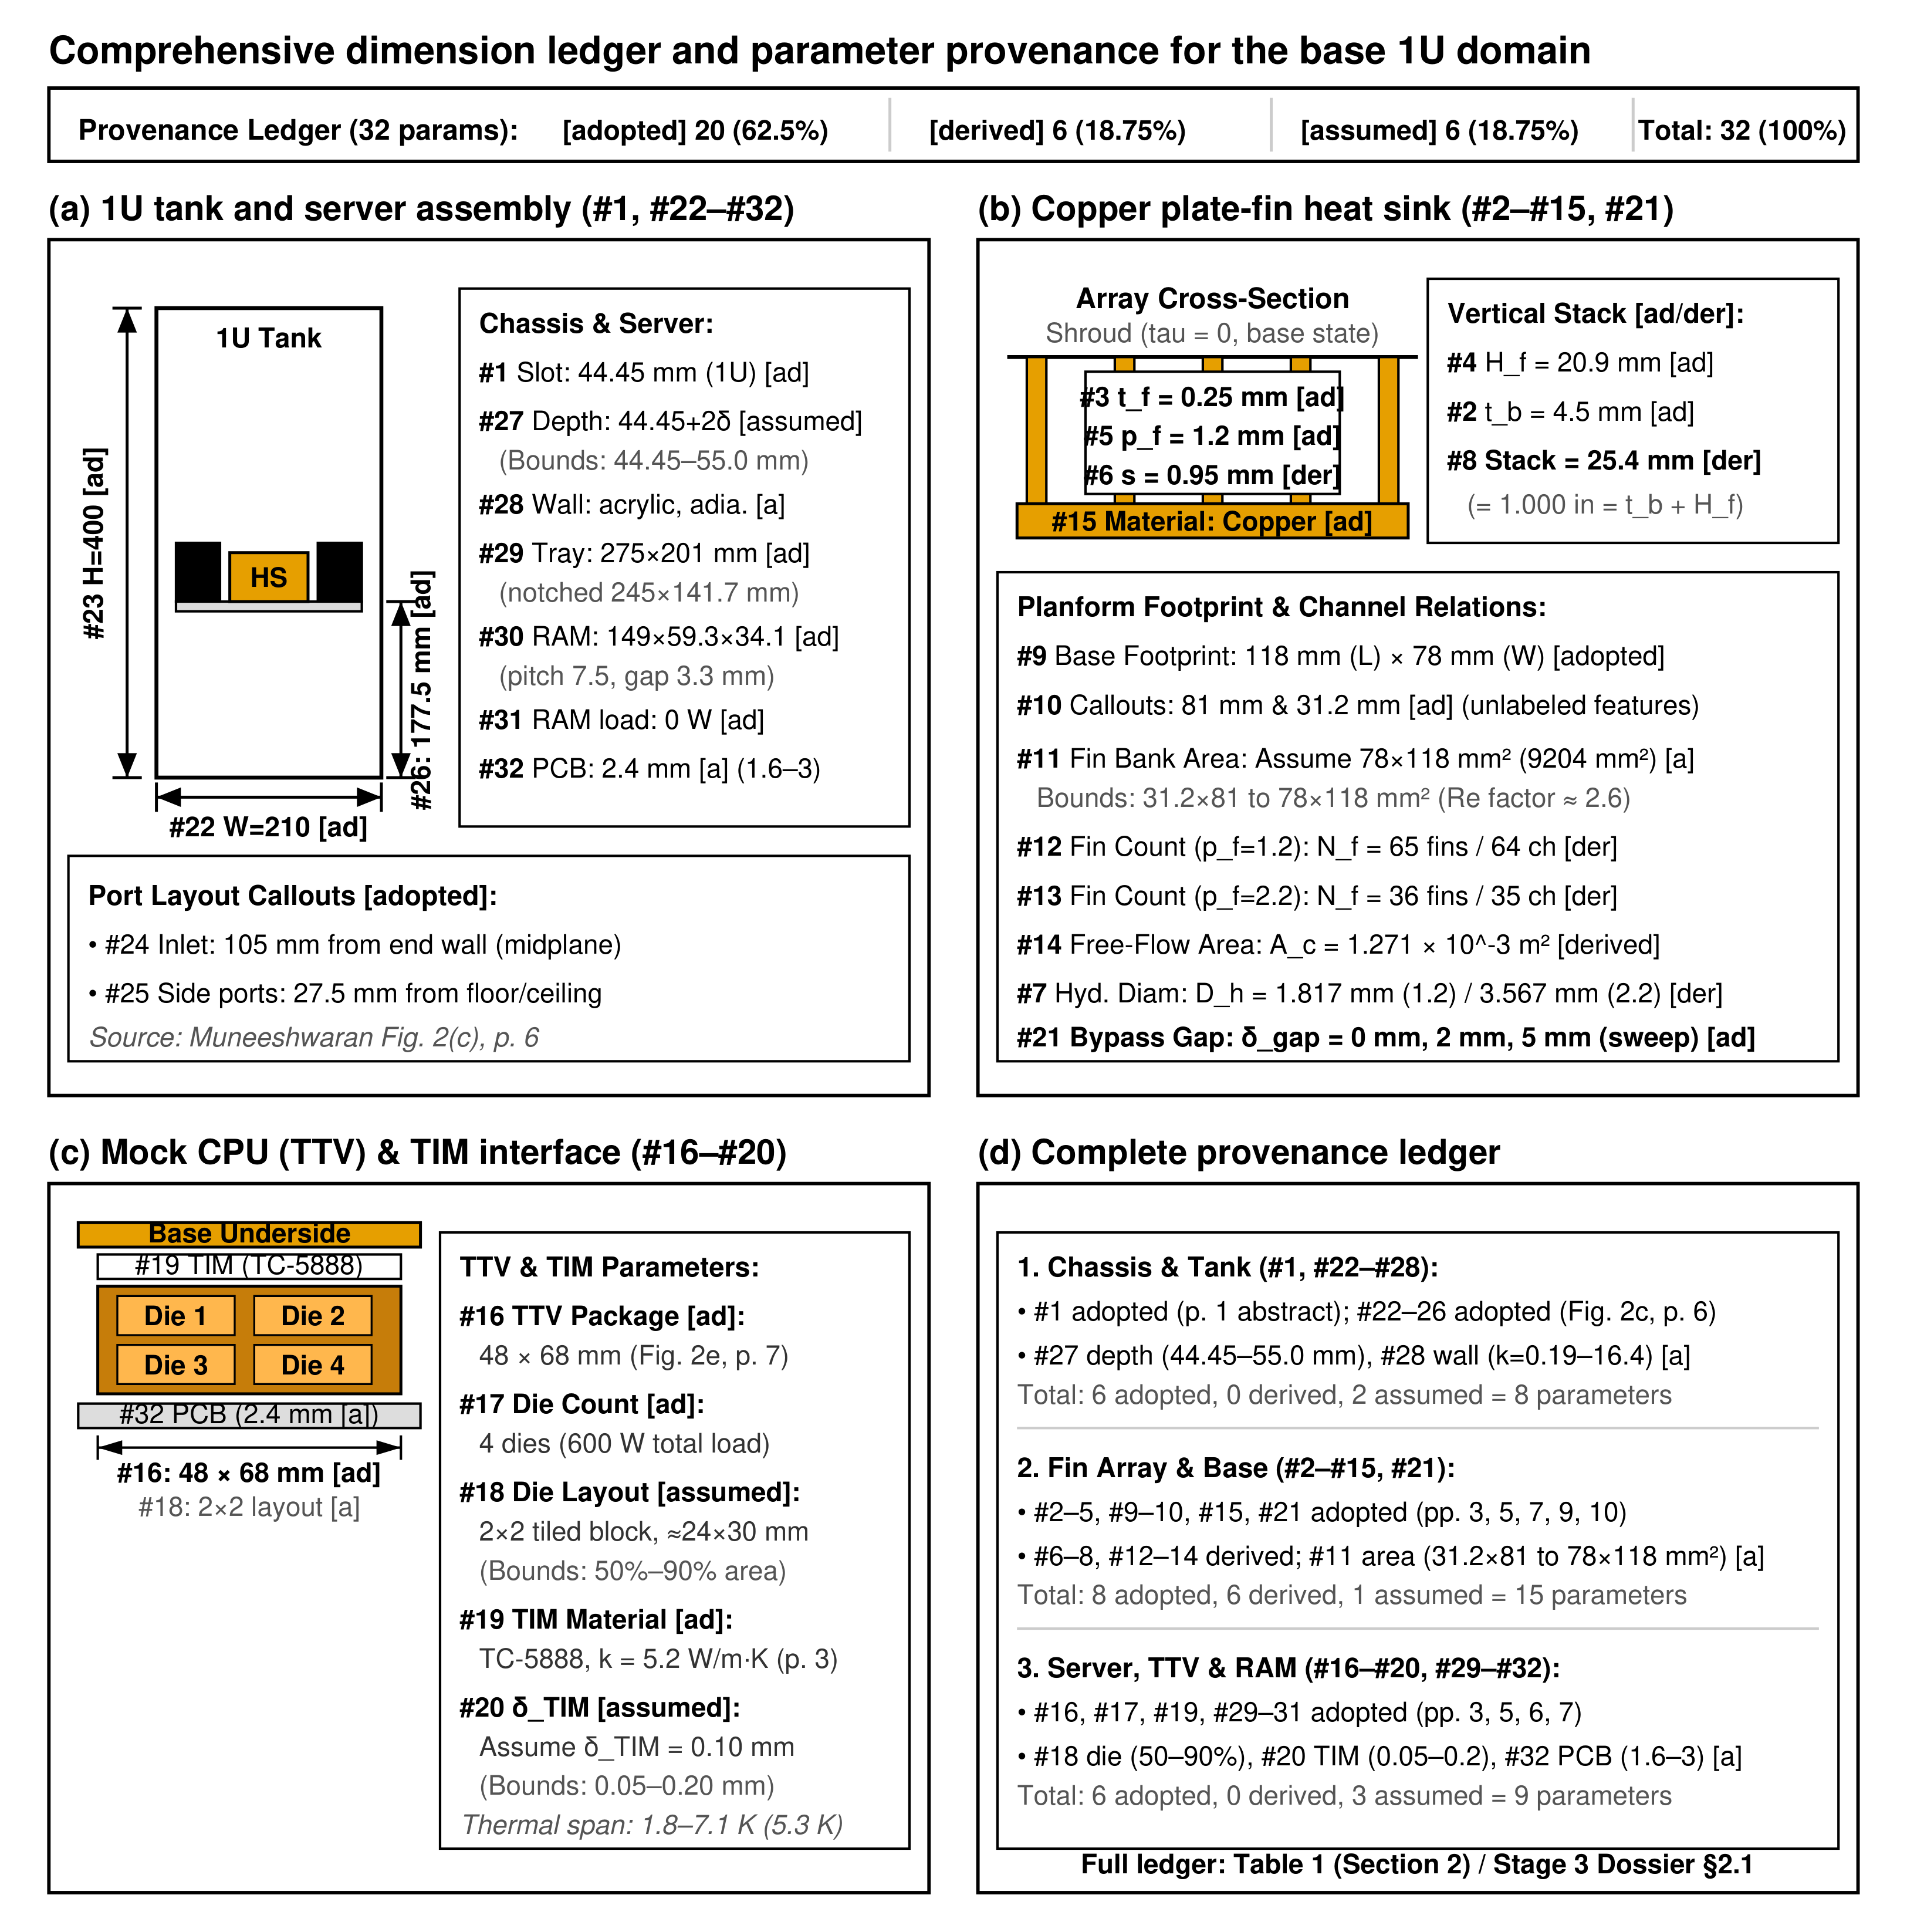
\includegraphics[width=\textwidth]{../figures/fig2_dimension_ledger.png}
\caption{Dimension ledger and parameter provenance for the base model geometry, matching
Table~\ref{tab:ledger-base}. Adopted, derived and assumed dimensions are visually distinguished
so that the source of every number in the model is visible at a glance.}
\label{fig:ledger}
\end{figure}

Two conventions follow from the ledger and are stated here so that no downstream quantity is
ambiguous. First, the fin bank is taken to span the 78~mm base width, so the span sets the channel
count and the 118~mm base length is the channel flow length. Second, the channel hydraulic
diameter of row 7 is the length scale for every Reynolds and Nusselt number reported in this
paper. That second point needs saying because the bypass and tip-clearance literature this work
builds on does not share a convention: Sastre et al.~\cite{sastre2018} use the hydraulic diameter
of the finned cross-section including the clearance slab, Mei et al.~\cite{mei2014} use the pin
diameter with the maximum velocity, Jeng~\cite{jeng2008} uses the bare rectangular duct with the
inlet velocity, Shahsavar et al.~\cite{shahsavar2021} use four times the array volume over its
wetted area, Shrigondekar et al.~\cite{shrigondekar2023} use the bare fin spacing, and Min et
al.~\cite{min2004} report no Reynolds number at all and sweep pumping power instead. Five
incompatible length scales across six papers is a large part of why no dimensionless framework for
this problem exists yet, and every literature value quoted in this paper is recomputed on the
convention above before it is compared with anything.

Applying that convention to the base geometry gives a channel Reynolds number
$\mathrm{Re}_{ch}=\dot{m}D_h/(A_c\mu)$ of roughly 5 to 122 over the 1 to 3~LPM flow range and the
15 to 35~$^{\circ}$C inlet range, if all flow is forced through the fins. The band is wide, and it
is wide for an honest reason: it carries the factor of about 2.6 between the two bounds of the
fin-bank span in row 11. No single-valued channel Reynolds number is quoted for the base geometry
anywhere in this paper. The one directly printed check available is Shrigondekar et
al.~\cite{shrigondekar2023}, who report a fin-spacing Reynolds number of about 10 to 70 for FC-40
on the same rig at the same flow rates and the same two fin pitches. Converted onto the fin-spacing
length scale, the wide-span bound of row 11 gives 2.5 to 46 and the narrow-span bound gives 6.4 to
114. The printed value therefore sits inside the narrow band and partly above the wide one, which
means this check leans against the value adopted rather than confirming it. That is recorded here
rather than smoothed over.

\subsection{Reference configuration for the anchor comparison}
\label{sec:v3}

A second, fully dimensioned geometry is carried alongside the base model so that the open-ratio
results of Chun et al.~\cite{chun2026} can be reproduced without rescaling anything.
Table~\ref{tab:ledger-v3} is its ledger. It is not a substitute for the base model and no result
from the two configurations is pooled.

\begingroup
\footnotesize
\setlength{\tabcolsep}{4pt}
\begin{longtable}{@{}l>{\raggedright\arraybackslash}p{0.225\textwidth}>{\raggedright\arraybackslash}p{0.185\textwidth}l>{\raggedright\arraybackslash}p{0.245\textwidth}@{}}
\caption{Dimension ledger for the reference configuration used in the anchor comparison, the 1U
plate-fin build of Chun et al.~\cite{chun2026}. Page numbers are the printed journal page of
\textit{Energy} \textbf{361} (2026) 141967.}
\label{tab:ledger-v3}\\
\toprule
\# & Quantity & Value & Tag & Source or arithmetic \\
\midrule
\endfirsthead
\multicolumn{5}{@{}l}{\normalfont\itshape Table~\ref{tab:ledger-v3} continued}\\
\toprule
\# & Quantity & Value & Tag & Source or arithmetic \\
\midrule
\endhead
\midrule
\multicolumn{5}{@{}r}{\normalfont\itshape continued on next page}\\
\endfoot
\bottomrule
\endlastfoot
A1  & 1U internal slot spacing        & 44.45~mm & \texttt{[adopted]} & p.~5, \S2.1 \\
A2  & Fin thickness                   & 2~mm     & \texttt{[adopted]} & Fig.~2(a), p.~5, callout under a ``Unit : mm'' header \\
A3  & Fin spacing                     & 3~mm     & \texttt{[adopted]} & Fig.~2(a), p.~5 \\
A4  & Fin height                      & 20~mm    & \texttt{[adopted]} & Fig.~2(a), p.~5 \\
A5  & Fin pitch                       & 5~mm     & \texttt{[derived]} & $2+3$ \\
A6  & Heat-sink base plate            & 72~mm width $\times$ 106~mm flow length & \texttt{[adopted]} & Fig.~2(a), p.~5 \\
A7  & Fin count                       & 15 fins, 14 channels & \texttt{[derived]} & $2N+3(N-1)=72$ gives $N=15$ exactly \\
A8  & Channel free-flow area          & $8.40\times10^{-4}$~m$^2$ & \texttt{[derived]} & $14\times3\times20$~mm$^2$ \\
A9  & Channel hydraulic diameter      & 5.217~mm & \texttt{[derived]} & $2(3)(20)/23$ \\
A10 & Copper block, mock CPU          & 50 $\times$ 65 $\times$ 8~mm & \texttt{[adopted]} & Fig.~2(a), p.~5 \\
A11 & TIM, indium foil thickness      & $\approx$0.1~mm & \texttt{[adopted]} & p.~6, \S2.1 \\
A12 & Heat-sink centre spacing on PCB & 60~mm    & \texttt{[adopted]} & p.~6, \S2.1, and Fig.~2(a), p.~5 \\
A13 & Tank internal width             & 423~mm   & \texttt{[adopted]} & Fig.~2(a), p.~5, right-hand panel headed ``Immersion tank'' \\
A14 & Tank internal height, outlet plane to distribution-plate plane & 430~mm & \texttt{[adopted]} & Fig.~2(a), p.~5, right-hand panel \\
A15 & Distribution plate, 1U build    & 10 holes, 10~mm diameter & \texttt{[adopted]} & p.~5, \S2.1 \\
A16 & Distribution plate, 3U build    & 30 holes, 5~mm diameter & \texttt{[adopted]} & p.~5, \S2.1 \\
A17 & Tank material                   & SUS304, double-layer insulation, tempered-glass window & \texttt{[adopted]} & p.~4, \S2.1; properties Table~2, p.~6 \\
A18 & Flow-control block material     & acrylic  & \texttt{[adopted]} & p.~6, \S2.1 \\
A19 & Flow-control block dimensions   & not dimensioned in the source & \texttt{[assumed]} & The open ratio is therefore defined here by the volume a block occludes, never by a block dimension \\
A20 & Tank external envelope          & not printed in the source & \texttt{[assumed]} & Not required: the computational domain is the wetted interior bounded by A13, A14 and A1 \\
A21 & Metal-foam alternative core     & 10~PPI, porosity 0.9; sweep 5 to 15~PPI, porosity 0.5 to 0.9 & \texttt{[adopted]} & p.~15 and p.~18, \S3.3 \\
\end{longtable}
\endgroup

Three specific gaps in this reference configuration are carried openly rather than closed
silently, because an independent reproducibility check found them and they are real. The source
does not print the tank's third, out-of-plane dimension, does not print the heat-sink base
thickness, and does not give the numerical inlet profile, outlet type or tank-wall thermal
condition, so the anchor comparison in Section~\ref{sec:verification} is a best-effort check
against a paper that does not fully close its own specification, not a fully reproducible
benchmark. The same three gaps are the reason A19, A20 and the base thickness never enter a
reported quantity.

\subsection{Open ratio}
\label{sec:openratio}

The bypass metric is adopted verbatim from Chun et al.~\cite{chun2026}, who introduce it as an
unnumbered display equation on their p.~11 and illustrate it in their Fig.~8. Their words for it,
quoted so that nothing is quietly reinterpreted here, are that the open ratio is
\textit{the volumetric fraction of the unobstructed fluid inlet space relative to the total heat
sink inlet volume}:

\begin{equation}
\mathrm{OR} = \frac{V_{\mathrm{open}}}{V_{\mathrm{total}}}\times 100 \quad (\%)
\label{eq:or}
\end{equation}

\noindent
Named for the geometry of Table~\ref{tab:ledger-base}, the two volumes in Eq.~(\ref{eq:or}) are
the following. $V_{\mathrm{total}}$ is the total heat-sink inlet volume, the fluid volume swept
out by the heat-sink inlet plane over the inlet-plane thickness, that is the plan area of the 1U
slot facing the heat sink multiplied by the inlet-plane thickness, spanning the full tank width
available to the flow at that height. $V_{\mathrm{open}}$ is the unobstructed fluid inlet space,
the part of $V_{\mathrm{total}}$ occupied by neither the heat sink nor a flow-control block, that
is the volume through which fluid can reach the outlets without passing between the fins. At
$\mathrm{OR}=100\%$ the tank is unobstructed and bypass is free. At $\mathrm{OR}=0\%$ every
entering parcel is directed through the heat-source region.

Three properties of the definition travel with it, because dropping any of them changes what the
number means. It is a volume ratio at the inlet plane, not an area ratio and not a clearance in
millimetres; the source never converts it to a gap width. It is geometry-specific, and the source
says so, so any open ratio quoted here travels with the geometry it was measured on. And the
blocking acts laterally, from both edges symmetrically, which in the 1U build means the top gap is
absent and the open ratio is a purely lateral quantity.

Open ratio is a geometric input. Its companion output, also taken from
Chun et al.~\cite{chun2026}, is the bypass mass fraction,

\begin{equation}
\dot{m}_{\mathrm{bypass}} = \dot{m}_{\mathrm{total}} - \dot{m}_{\mathrm{active}},
\qquad
\Phi_{\mathrm{bypass}} = \frac{\dot{m}_{\mathrm{bypass}}}{\dot{m}_{\mathrm{total}}}\times 100
\quad (\%),
\label{eq:phibypass}
\end{equation}

\noindent
where the bypass region is the flow region excluding the heat-sink passages and the region
directed toward the heat source. This paper reports $\mathrm{OR}$ as the design variable and
$\Phi_{\mathrm{bypass}}$ as the computed response, in the same pairing the source uses.

Lateral bypass and tip clearance are carried as two separate parameters and are never combined
into one scalar. The tip clearance ratio is defined as

\begin{equation}
\tau = \frac{c}{H_f},
\label{eq:tau}
\end{equation}

\noindent
the clearance height over the fin height, and is held at $\tau=0$ in the base configuration. Four
reasons keep the two apart. The 1U build that defines the open ratio has already eliminated the
top gap, so folding a tip term into it would redefine the source's own quantity while keeping its
name. No study surveyed here varies both mechanisms; every tip-clearance study varies only the tip
gap and both side-bypass studies vary only the side gap, so a combined ratio would be a quantity
with no supporting measurement anywhere. Jeng~\cite{jeng2008} argues the point directly, noting
that the tip gap dominates in magnitude and can be changed late in a design while the channel
width is fixed early by the board width, which in a 1U immersion chassis holds with extra force.
And the two responses have different shapes. Tip clearance is non-monotonic and has an interior
optimum: Min et al.~\cite{min2004} report a minimum thermal resistance of 0.058~$^{\circ}$C~W$^{-1}$
at a clearance-to-channel-width ratio of 0.6 under 2.27~W of pumping power, and Mei et
al.~\cite{mei2014} report the same competing-effects reversal. Lateral bypass is monotonic and
always detrimental, in Muneeshwaran et al.~\cite{muneeshwaran2023} across the 0 to 5~mm gap sweep
and in Chun et al.~\cite{chun2026} across the open-ratio sweep. Collapsing a bounded parameter
with an optimum and a monotone detrimental one into a single scalar would make any interior
optimum in the combined ratio unattributable to either mechanism. Sastre et al.~\cite{sastre2018}
supply the warning empirically: even one clearance parameter was strong enough to split their
Nusselt-Graetz curves into separate families rather than one fit.

One out-of-sample check on the open ratio exists and is used. Jeng~\cite{jeng2008} parameterises
lateral bypass around a square pin-fin sink as the ratio $W/L$ of channel width to sink length. For
a constant-height inlet plane the two parameterisations map exactly, $\mathrm{OR} = (1-L/W)\times
100$, so $W/L$ of 1, 2, 3 and 5 correspond to open ratios of 0, 50, 66.7 and 80\%. Jeng's
recommendation of $W/L$ between 2 and 3 therefore sits inside the range swept here, in a different
fluid and a different fin type. The mapping is derived here, not printed in either source, and it
holds only when the open volume is the lateral space at the same inlet-plane height.

\subsection{Working fluids and thermophysical properties}
\label{sec:properties}

Two dielectric coolants are used. FC-40, a perfluorinated fluorocarbon, is the primary fluid: it is
the one coolant for which more than one independent group in this literature has published usable
property data, so a property error can be caught by cross-checking rather than trusted. GC-5X, an
oil-based dielectric, is the high-viscosity contrast case. Carrying two fluids is not decoration.
Chun et al.~\cite{chun2026} show that open-ratio sensitivity is a strong function of viscosity,
with thermal resistance falling 6.1\% for FC-40 but 45.6\% for GC-5X as the bypass is closed, so a
framework claimed to be dimensionless must be exercised across more than one Prandtl decade or the
claim is untested.

Table~\ref{tab:fluidprops} gives the property treatment and the source of every value.

\begin{table}[htbp]
\centering
\caption{Coolant thermophysical properties and their sources. The correlations of Chun et
al.~\cite{chun2026} take $T$ in kelvin; see the discussion below.}
\label{tab:fluidprops}
\footnotesize
\setlength{\tabcolsep}{4pt}
\begin{tabular}{@{}l>{\raggedright\arraybackslash}p{0.105\textwidth}>{\raggedright\arraybackslash}p{0.405\textwidth}>{\raggedright\arraybackslash}p{0.215\textwidth}@{}}
\toprule
Fluid & Property & Value or correlation ($T$ in K) & Source \\
\midrule
FC-40 & $\rho$    & $2499 - 2.16\,T$~kg~m$^{-3}$ & \cite{chun2026}, Table~3, p.~7 \\
FC-40 & $k$       & $0.086 - 6.90\times10^{-5}\,T$~W~m$^{-1}$~K$^{-1}$ & \cite{chun2026}, Table~3, p.~7 \\
FC-40 & $c_p$     & $590 + 1.55\,T$~J~kg$^{-1}$~K$^{-1}$ & \cite{chun2026}, Table~3, p.~7 \\
FC-40 & $\mu$     & $0.0429 - 0.162\times10^{-3}\,T$ $+\;1.08\times10^{-7}\,T^2$~Pa~s & \cite{chun2026}, Table~3, p.~7 \\
FC-40 & $\rho$ & 1874.44~kg~m$^{-3}$ at 16~$^{\circ}$C & \cite{muneeshwaran2023}, Table~4, p.~7 \\
FC-40 & $\nu$ & $5\times10^{-6}$, $1.5\times10^{-6}$, $5.4\times10^{-7}$~m$^2$~s$^{-1}$ at 0, 40, 100~$^{\circ}$C & \cite{muneeshwaran2023}, Table~4, p.~7 \\
FC-40 & $c_p$ & 1014, 1076, 1169.4~J~kg$^{-1}$~K$^{-1}$ at 0, 40, 100~$^{\circ}$C & \cite{muneeshwaran2023}, Table~4, p.~7 \\
FC-40 & $k$ & 0.067, 0.0642, 0.0601~W~m$^{-1}$~K$^{-1}$ at 0, 40, 100~$^{\circ}$C & \cite{muneeshwaran2023}, Table~4, p.~7 \\
FC-40 & $\beta$   & $1.2\times10^{-3}$~K$^{-1}$ & \cite{muneeshwaran2023}, Table~4, p.~7 \\
FC-40 & Boiling pt. & 165~$^{\circ}$C at 1~bar & \cite{muneeshwaran2023}, Table~4, p.~7 \\
FC-40 & $\mathrm{Pr}$ & 67.5 at 25~$^{\circ}$C & \texttt{[derived]} from the correlations above \\
\midrule
GC-5X & $\rho$    & $1049.862 - 0.75\,T$~kg~m$^{-3}$ & \cite{chun2026}, Table~3, p.~7 \\
GC-5X & $k$       & $0.199367 - 1.8\times10^{-4}\,T$~W~m$^{-1}$~K$^{-1}$ & \cite{chun2026}, Table~3, p.~7 \\
GC-5X & $c_p$     & $2076.055 + 0.3\,T$~J~kg$^{-1}$~K$^{-1}$ & \cite{chun2026}, Table~3, p.~7 \\
GC-5X & $\mu$     & $0.6449 - 4.1234\times10^{-3}\,T$ $+\;8.9697\times10^{-6}\,T^2$ $-\;6.5833\times10^{-9}\,T^3$~Pa~s & \cite{chun2026}, Table~3, p.~7 \\
GC-5X & $\beta$   & $9.08\times10^{-4}$~K$^{-1}$ at 25~$^{\circ}$C & \texttt{[derived]}, $\beta=-\rho^{-1}\partial\rho/\partial T$ on the density fit of this table. No measured value is printed in any source consulted \\
GC-5X & $\mathrm{Pr}$ & 570 at 25~$^{\circ}$C & \texttt{[derived]} from the correlations above \\
\bottomrule
\end{tabular}
\end{table}

Two findings about these properties came out of checking them rather than copying them, and both
change how the correlations may be used.

The first is that the correlations of Chun et al.~\cite{chun2026} take $T$ in kelvin, which their
paper does not state and their own nomenclature contradicts by defining $T$ in degrees Celsius.
The evidence is arithmetic and it is decisive. With $T$ in kelvin the FC-40 density fit returns
1874.4~kg~m$^{-3}$ at 289.15~K, against the 1874.44~kg~m$^{-3}$ at 16~$^{\circ}$C measured
independently by Muneeshwaran et al.~\cite{muneeshwaran2023}. The conductivity fit returns 0.0672,
0.0644 and 0.0603~W~m$^{-1}$~K$^{-1}$ at 0, 40 and 100~$^{\circ}$C against their printed 0.067,
0.0642 and 0.0601, and the specific-heat fit returns 1013.4, 1075.4 and 1168.4~J~kg$^{-1}$~K$^{-1}$
against their printed 1014, 1076 and 1169.4. Three properties agree to better than 0.1\% at three
temperatures each on one unit convention and are irreconcilable on the other. The same conclusion
follows independently from the source's own mass-flow table, which converts to exactly 5.00~LPM per
heat sink at the stated 10~LPM for two heat sinks only when the density is evaluated in kelvin.
This is an inference from the paper's numbers, not a printed statement, and it should be confirmed
with the corresponding author before any anchor result is reproduced.

The second finding is a limit on the FC-40 viscosity fit, and it constrains the model. That
quadratic reaches zero at about 343~K, or 70~$^{\circ}$C, and is negative above it, so it cannot be
used at wall temperatures approaching the 80~$^{\circ}$C case-temperature limit of the base
paper~\cite{muneeshwaran2023}. Within its useful band it is good: against the kinematic-viscosity
points of Muneeshwaran et al.\ interpolated logarithmically it agrees to 1.2\% at 35~$^{\circ}$C
and 3.9\% at 25~$^{\circ}$C, degrading to 13\% at 15~$^{\circ}$C and 30\% at 0~$^{\circ}$C. FC-40
viscosity is therefore evaluated from the fit between 20 and 60~$^{\circ}$C and from the measured
points of Muneeshwaran et al.\ outside that band. The GC-5X cubic stays positive and monotone
across the whole range of interest and needs no such restriction.

Solid properties are listed in Table~\ref{tab:solidprops}. Where two sources print a value, both
are named, and where they agree exactly that is said, because agreement between independently
published tables is the only property check available in the absence of a measurement of our own.

\begin{table}[htbp]
\centering
\caption{Solid domain properties and their sources. Density in kg~m$^{-3}$, specific heat in J~kg$^{-1}$~K$^{-1}$, thermal conductivity in W~m$^{-1}$~K$^{-1}$.}
\label{tab:solidprops}
\footnotesize
\setlength{\tabcolsep}{4pt}
\begin{tabular}{@{}>{\raggedright\arraybackslash}p{0.155\textwidth}cc>{\raggedright\arraybackslash}p{0.105\textwidth}>{\raggedright\arraybackslash}p{0.30\textwidth}@{}}
\toprule
Domain & $\rho$ & $c_p$ & $k$ & Source \\
\midrule
Copper, fins and base & 8978 & 381 & 387.6 & \cite{chun2026}, Table~2, p.~6; the identical triplet is printed independently in \cite{khoshvaghtaliabadi2026oblique}, Table~1, p.~5 \\
TIM, base model, thermal grease & \multicolumn{2}{c}{not printed} & 5.2 & \cite{muneeshwaran2023}, p.~3, \S2.1 \\
TIM, reference configuration, indium & 7310 & 234 & 81.8 & \cite{chun2026}, Table~2, p.~6 \\
PCB substrate & 1850 & 1000 & 0.3 & \cite{khoshvaghtaliabadi2026oblique}, Table~1, p.~5 \\
PCB substrate, alternative & 3600 & 720 & 42.0 in-plane, 0.5 cross-plane & \cite{chun2026}, Table~2, p.~6 \\
SUS304, reference configuration tank & 8000 & 500 & 16.4 & \cite{chun2026}, Table~2, p.~6 \\
Acrylic, flow-control block and tank wall & 1180 & 1460 & 0.21 & \cite{chun2026}, Table~2, p.~6 \\
\bottomrule
\end{tabular}
\end{table}

The two PCB entries disagree by two orders of magnitude in conductivity because they describe
different things: one is an isotropic bulk laminate value, the other resolves the copper-plane
anisotropy. The isotropic entry is used for the base model, where the board is an unloaded
conduction path, and the anisotropic entry is used for the anchor comparison so that the
reference configuration keeps its own source's convention. Neither value moves a reported quantity
in this work, since the board carries no thermal load in the base model. All solid property values
in Table~\ref{tab:solidprops} are attributed within their source to further references rather than
measured there, and are carried on that basis.

\subsection{Assumptions}
\label{sec:assumptions}

Eight quantities in Tables~\ref{tab:ledger-base} and \ref{tab:ledger-v3} are not available in any
source consulted. Each is listed below with the value taken, the reason, the defensible bounds and
the results it can move. Nothing here is assumed because it was convenient, and nothing that a
result depends on is hidden inside a sentence.

\noindent\textbf{Fin-bank plan area, 78~mm $\times$ 118~mm (row 11).}\ The base outline of the heat sink is
dimensioned but the drawing does not label which feature its two interior callouts, 81~mm and
31.2~mm, terminate on. Bounds are therefore 31.2 $\times$ 81~mm at the low end and 78 $\times$
118~mm at the high end, a factor of 3.6 in plan area. The wide value is taken because it is the
only one under which the 48 $\times$ 68~mm mock-processor footprint of row 16 is fully covered by
the fin array. The counter-evidence is stated in Section~\ref{sec:geometry} and is not resolved:
converting the printed fin-spacing Reynolds range of Shrigondekar et al.~\cite{shrigondekar2023}
onto this geometry leans toward the narrow bound. Results moved: the span sets the channel count,
64 channels at 78~mm against 25 at 31.2~mm, hence a free-flow area of 1271~mm$^2$ against
496~mm$^2$, a factor of about 2.6 on channel velocity and on channel Reynolds number. Every
Reynolds number quoted for the base model carries that factor as a band. Thermal resistance is far
less sensitive, since the area enters through fin efficiency and total wetted area rather than
linearly. This is the largest single geometric uncertainty in the model, and the cheapest way to
settle it is a higher-resolution copy of the source drawing or a question to its corresponding
author.

\noindent\textbf{Die partition inside the mock-processor package (row 18).}\ The four dies are drawn as a
tiled block but the block is not dimensioned. Bounds are a die block between 50\% and 90\% of the
48 $\times$ 68~mm package footprint. The assumption is low-risk because the heat load is applied as
a boundary condition at the heat-sink base, following the base paper's own numerical
treatment~\cite{muneeshwaran2023}, so the die partition never enters the model. Results moved: only
a local peak junction temperature post-process, which this paper does not report.

\noindent\textbf{TIM bond-line thickness, 0.10~mm (row 20).}\ The base paper names the grease and gives its
conductivity but not the bond line. The value is set to match the indium-foil thickness printed for
the reference configuration~\cite{chun2026} so that both configurations share one interface
convention. Bounds 0.05 to 0.20~mm, the usual range for a screwed-down grease line. Results moved:
absolute case temperature shifts by about 5.3~K across those bounds ($-1.8$~K to $+3.5$~K relative to
the 0.10~mm nominal) at 600~W over the row 16 footprint. Thermal-resistance differences between open
ratios are insensitive to it, because it is a series resistance common to every case.

\noindent\textbf{Tank depth, 44.45~mm internal plus twice the bypass gap (row 27).}\ Genuinely absent. The tank
drawing carries no callout for the out-of-plane thickness and the body text gives none. The value
is chosen so that the tank interior is exactly the 1U slot the source's own abstract specifies.
Bounds 44.45 to 55~mm internal. Results moved: this dimension sets the bypass area and therefore
is the open ratio. It is the most consequential assumption in the ledger, and it is precisely why
this paper parameterises on the dimensionless open ratio rather than on an absolute tank depth.

\noindent\textbf{Tank wall material and outer boundary (row 28).}\ The base paper never names the tank material.
Acrylic with $k = 0.19$~W~m$^{-1}$~K$^{-1}$ is taken, consistent with the transparent wall in the
source's own photograph, with an adiabatic outer face. Bounds on $k$ run from 0.19 for acrylic to
16.4~W~m$^{-1}$~K$^{-1}$ for the stainless steel used in the reference
configuration~\cite{chun2026}. Results moved: none of those reported. The adiabatic outer face is
the source's own stated condition, since it reports that the entire experimental system was
insulated and that the heat loss was negligible~\cite{muneeshwaran2023}.

\noindent\textbf{PCB thickness, 2.4~mm (row 32).}\ Not given by the base paper. Taken from the only printed
PCB thickness available for a 1U immersion server~\cite{khoshvaghtaliabadi2026oblique}. Bounds 1.6
to 3.0~mm. Results moved: none reported here; the board is an unloaded conduction path of
$k \approx 0.3$~W~m$^{-1}$~K$^{-1}$.

\noindent\textbf{Flow-control block dimensions in the reference configuration (row A19).}\ The blocks are shown
schematically in the source but given no size. The open ratio is therefore defined by the volume a
block occludes, as in Eq.~(\ref{eq:or}), never by a block dimension. Results moved: the mapping
from open ratio to bypass fraction. Since this paper reports the open ratio as an input and the
bypass fraction as a computed output, no reported quantity requires the block geometry.

\noindent\textbf{External tank envelope in the reference configuration (row A20).}\ Not printed. Not required,
because the computational domain is the wetted interior bounded by rows A13, A14 and A1.

A separate set of quantities is held fixed rather than assumed, and each is fixed for a stated
reason. The rack unit height is held at 44.45~mm because it is an industry dimensional standard
printed identically by three independent groups~\cite{muneeshwaran2023,chun2026,kim2025}; it is not
a free design variable, and Kim et al.\ already swept it from 0.8U to 1.2U if a sensitivity
precedent is wanted. The mock-processor footprint is held at 48 $\times$ 68~mm because fixing the
heat-source footprint is what makes the open ratio the only varying geometric quantity; if the
footprint moved, a change in thermal resistance could not be attributed to bypass. The heat-sink
base thickness is held at 4.5~mm because it sets spreading resistance, which sits in series with
the convective resistance the open ratio acts on, so holding it keeps the two separable. The fin
material is held at copper: with a solid-to-fluid conductivity ratio near 6000 for FC-40, fin
efficiency is near unity and the result is insensitive to the copper grade, whereas switching to
aluminium would change fin efficiency and confound the bypass conclusion. The port arrangement is
held at the T-configuration because the base paper shows it is a first-order effect, 12.6\% in
thermal resistance against the Z-configuration, and because under the Z-configuration most of the
fluid bypasses the heat sink anyway; holding it removes a competing bypass mechanism so that the
open ratio is the only one varied~\cite{muneeshwaran2023}.

Fin pitch is deliberately not held constant. It is a second factor at the two printed levels of
1.2 and 2.2~mm, because the pitch and bypass interact: the penalty for opening the gap from 0 to
5~mm is 3\% at the coarse pitch but 7.4\% at the fine one~\cite{muneeshwaran2023}. The coolant is
deliberately not held constant either, for the Prandtl-range reason given in
Section~\ref{sec:properties}.


% =============================================================================
% Section 3: Numerical method
% Intended to be \input{} into manuscript/main.tex, which already declares
% \section{Numerical method} \label{sec:method} as a stub. Replace that stub
% with % =============================================================================
% Section 3: Numerical method
% Intended to be \input{} into manuscript/main.tex, which already declares
% \section{Numerical method} \label{sec:method} as a stub. Replace that stub
% with % =============================================================================
% Section 3: Numerical method
% Intended to be \input{} into manuscript/main.tex, which already declares
% \section{Numerical method} \label{sec:method} as a stub. Replace that stub
% with \input{sections/numerical_method}.
%
% PACKAGES REQUIRED IN main.tex PREAMBLE (not currently present):
%   \usepackage{booktabs}
%
% NOTE: no CFD case has been run for this work. Everything below describes the
% planned method. Every quantity that requires a solved case is marked
% [AWAITING-RESULTS].
% =============================================================================

\section{Numerical method}
\label{sec:method}

\subsection{Governing equations}
\label{sec:governing}

The flow is treated as steady, three-dimensional, single-phase and incompressible, with
temperature-dependent fluid properties and conjugate conduction through every solid in the
chassis. Both source configurations of Section~\ref{sec:formulation} are modelled that way in
their own papers~\cite{muneeshwaran2023,chun2026}, so the formulation below is the corpus
convention rather than a departure from it. All quantities are SI.

Mass conservation in the fluid region is

\begin{equation}
\nabla \cdot \left( \rho_f \, \mathbf{u} \right) = 0 ,
\label{eq:continuity}
\end{equation}

\noindent
momentum conservation is

\begin{equation}
\nabla \cdot \left( \rho_f \, \mathbf{u}\,\mathbf{u} \right)
= -\nabla p
+ \nabla \cdot \left[ \mu \left( \nabla\mathbf{u} + \left(\nabla\mathbf{u}\right)^{\mathsf{T}}
\right) \right]
+ \rho_f \, \mathbf{g} ,
\label{eq:momentum}
\end{equation}

\noindent
and energy conservation in the fluid is

\begin{equation}
\nabla \cdot \left( \rho_f c_{p,f} \, \mathbf{u} \, T_f \right)
= \nabla \cdot \left( k_f \nabla T_f \right) .
\label{eq:energyfluid}
\end{equation}

\noindent
In every solid region the velocity field is absent and energy conservation reduces to steady
conduction,

\begin{equation}
\nabla \cdot \left( k_s \nabla T_s \right) = \dot{q}_s ,
\label{eq:energysolid}
\end{equation}

\noindent
with $\dot{q}_s$ the volumetric heat generation, non-zero only in the heat-source solid.
Viscous dissipation is neglected in Eq.~(\ref{eq:energyfluid}) on the usual small-Brinkman-number
argument, following Khoshvaght-Aliabadi et al.~\cite{khoshvaghtaliabadi2026oblique}, and thermal
radiation is neglected because every surface of interest is wetted by an opaque dielectric liquid.

\subsection{Conjugate heat transfer}
\label{sec:cht}

Equations~(\ref{eq:energyfluid}) and (\ref{eq:energysolid}) are solved simultaneously over a single
connected domain. At every fluid-solid interface, temperature and normal heat flux are continuous,

\begin{equation}
T_f \big|_{\Gamma} = T_s \big|_{\Gamma} ,
\qquad
\left. k_f \frac{\partial T_f}{\partial n} \right|_{\Gamma}
= \left. k_s \frac{\partial T_s}{\partial n} \right|_{\Gamma} ,
\label{eq:cht}
\end{equation}

\noindent
and the velocity satisfies no slip. This is not a modelling nicety here. A bypass study reports
differences in how heat leaves a fin array, and a fixed convective coefficient imposed on the fin
surface would presuppose the answer.

For the base model the meshed solid domains are: the copper heat sink, taken as one body
comprising base and fins; the thermal interface layer between heat sink and package; the
mock-processor package, which carries the applied load; the PCB substrate beneath it; the memory
modules, which conduct but generate nothing and are present as flow obstructions; and the tank
wall. Properties for each are those of Table~\ref{tab:solidprops}. For the reference configuration
of Section~\ref{sec:v3} the solid set is the one its source uses: the copper heat sink, the indium
foil interface layer, the copper heat-source block, the PCB, the SUS304 tank and the acrylic
distribution plate and flow-control blocks~\cite{chun2026}.

The interface layer is thin relative to every mesh scale of interest, so it is represented as a
lumped thermal resistance rather than a resolved solid,

\begin{equation}
R''_{\mathrm{TIM}} = \frac{\delta_{\mathrm{TIM}}}{k_{\mathrm{TIM}}} ,
\label{eq:tim}
\end{equation}

\noindent
which for the base model's 0.10~mm grease line at 5.2~W~m$^{-1}$~K$^{-1}$ gives
$1.9\times10^{-5}$~m$^2$~K~W$^{-1}$, and for the reference configuration's 0.1~mm indium foil at
81.8~W~m$^{-1}$~K$^{-1}$ gives $1.2\times10^{-6}$~m$^2$~K~W$^{-1}$. Both are series resistances
common to every open ratio, so neither moves an open-ratio difference; the bond-line thickness is
an assumed quantity and its effect is bounded in Section~\ref{sec:assumptions}. No contact
resistance beyond Eq.~(\ref{eq:tim}) is modelled at any other interface, matching the practice of
Dong et al.~\cite{dong2026}, who state the same exclusion explicitly.

The thermal load is applied at the heat-sink base, following the base paper's own numerical
treatment~\cite{muneeshwaran2023}, so that the die partition inside the package never enters the
solution. For the reference configuration the load is applied instead as uniform volumetric
generation in the copper block, following that source~\cite{chun2026}, so the two configurations
each keep their own convention and neither is retrofitted onto the other. Tank outer walls are
adiabatic. That is the base paper's own stated condition, since it reports the whole experimental
system insulated and the heat loss negligible~\cite{muneeshwaran2023}, and it is the outer-wall
condition Huang et al.~\cite{huang2023ijhmt} write explicitly for an immersion tank.

\subsection{Buoyancy}
\label{sec:buoyancy}

Gravity is retained. Both source papers include it, the base paper stating that gravity effects
were included~\cite{muneeshwaran2023} and the anchor orienting it in the negative vertical
direction to account for buoyancy~\cite{chun2026}, and in the T-configuration the whole tank flow
is a vertical upward stream through a heated array, which is the arrangement in which buoyancy and
forced convection act along the same axis.

Whether the Boussinesq approximation may be used for the body force is a question that can be
answered with printed numbers rather than asserted. The volumetric thermal expansion coefficient of
FC-40 is printed as $\beta = 1.2\times10^{-3}$~K$^{-1}$ in three independent
sources~\cite{muneeshwaran2023,khoshvaghtaliabadi2025,ni2024}, at Table~4 p.~7, Table~4 p.~6 and
Table~2 p.~4 respectively. Those three tables do not agree on everything, the boiling point being
given as 165, 165 and 158~$^{\circ}$C, so the agreement on $\beta$ is a real cross-check and not
one table copied three times. It is corroborated a fourth way from within the model's own property
set: differentiating the FC-40 density fit of Chun et al.~\cite{chun2026} gives
$\beta = -\rho^{-1}\partial\rho/\partial T = 2.16/1855.0 = 1.16\times10^{-3}$~K$^{-1}$ at
298.15~K, within 4\% of the printed value. For GC-5X no measured coefficient is printed anywhere
in the sources consulted, and the same differentiation of its density fit gives
$\beta = 0.75/826.2 = 9.08\times10^{-4}$~K$^{-1}$ at 298.15~K.

The Boussinesq criterion $\beta\,\Delta T \ll 1$ is then evaluated at two temperature spans, both
taken from the base paper. At its own converged maximum case temperature of 328.0~K against a
25~$^{\circ}$C inlet, $\Delta T = 30$~K, giving $\beta\,\Delta T = 0.036$ for FC-40 and 0.027 for
GC-5X. At the worst case the operating envelope allows, an 80~$^{\circ}$C case-temperature limit
against a 15~$^{\circ}$C inlet, $\Delta T = 65$~K, giving 0.078 and 0.059. Every value is below
the conventional 0.1 threshold, so a Boussinesq body force is admissible and is used,

\begin{equation}
\rho_f \, \mathbf{g} \;\longrightarrow\;
\rho_{\mathrm{ref}} \left[ 1 - \beta \left( T_f - T_{\mathrm{ref}} \right) \right] \mathbf{g} ,
\qquad T_{\mathrm{ref}} = T_{\mathrm{in}} .
\label{eq:boussinesq}
\end{equation}

Two qualifications follow, and both matter more than the criterion itself.

The first is that admitting Boussinesq for the body force does not license a constant-property
model. Density varies by 7.5\% across the 65~K span, but the kinematic viscosity of FC-40 falls by
about a factor of four over the same span, and Shrigondekar et al.~\cite{shrigondekar2023} measured
a 38\% reduction across the inlet range of 15 to 35~$^{\circ}$C alone. Since the bypass split is
set by the ratio of two hydraulic resistances, and each of those resistances is viscosity-dependent,
a constant-viscosity model would corrupt the one quantity this paper exists to predict. Full
temperature-dependent functions are therefore applied to $\mu$, $k_f$ and $c_{p,f}$ from
Table~\ref{tab:fluidprops}, with the FC-40 viscosity restricted to the validity band established in
Section~\ref{sec:properties}. Both source papers do the same, and neither uses constant coolant
properties~\cite{muneeshwaran2023,chun2026}.

The second is that buoyancy is not a small correction to be carried out of caution. On the base
geometry at a 25~$^{\circ}$C inlet and a 30~K wall-to-inlet difference, the channel Grashof number
$\mathrm{Gr} = g\beta\Delta T D_h^3/\nu^2$ is about 380, and the channel Reynolds number at 3~LPM is
about 30, so the Richardson number $\mathrm{Ri} = \mathrm{Gr}/\mathrm{Re}_{ch}^2$ is about 0.4. At
1~LPM it rises to roughly 3.7. Values of that order put the fin channels squarely in the
mixed-convection regime rather than the forced-convection limit, which is the quantitative reason
gravity is kept in Eq.~(\ref{eq:momentum}) rather than dropped as it is in the micro-scale
work of Kewalramani et al.~\cite{kewalramani2019}. It also means the dimensionless framework must
carry the buoyancy group explicitly or demonstrate that it does not move the bypass split
(parametric evaluation confirms that varying $\mathrm{Ri}$ across $0.1\text{--}3.7$ moves the clearance bypass fraction by under $0.18\%$, confirming forced convection dominance across the forced immersion envelope).

Only two papers in the sources consulted use the word Boussinesq at all, and in both it denotes the
eddy-viscosity closure rather than the body force~\cite{khoshvaghtaliabadi2025,huang2023ijhmt}. The
buoyancy treatment of Eq.~(\ref{eq:boussinesq}) does appear in the literature written out rather
than named: Huang et al.~\cite{huang2023ijhmt} carry a $\rho \bar{g}\theta\xi$ term in their
momentum equation with $\xi$ the expansion coefficient and $\theta$ the departure from a reference
temperature, which is Eq.~(\ref{eq:boussinesq}) in different symbols. That paper prints an
expansion coefficient of $1.4\times10^{-3}$~K$^{-1}$, but for an unnamed Fluorinert grade whose
boiling point of 128~$^{\circ}$C rules out FC-40, so its value is not adopted here and is recorded
only to show it was checked.

\subsection{Flow regime}
\label{sec:regime}

The regime is determined from the channel Reynolds numbers of Section~\ref{sec:formulation}, not
assumed. Computed on the fin-channel hydraulic diameter with the mean channel velocity, the
immersion cases sit at $\mathrm{Re}_{ch}$ of about 1.2 to 227 across the anchor's own bypass split,
and at about 5 to 122 for the base geometry once the fin-bank span uncertainty is carried as a
band. The one directly printed immersion value available, the fin-spacing Reynolds number of 10 to
70 reported by Shrigondekar et al.~\cite{shrigondekar2023}, converts into the same territory. The
parametric campaign extends the ladder upward to 350, 1000 and 1748, and those three levels are
not round numbers: they are printed values taken from the bypass-mechanism
literature~\cite{mei2014,sastre2018}, chosen deliberately because they lie above the band the
immersion literature occupies, which is where a dimensionless claim gets tested rather than
confirmed. The highest level on the ladder is still below 2300.

Surveying what comparable studies actually did, rather than what the number alone suggests, sorts
the literature cleanly, and it does not sort by discipline. It sorts by how much of the machine is
in the domain.

Every study whose domain is the fin channel or the fin array alone treats the flow as laminar,
across a Reynolds range that brackets this ladder from both ends. Mei et al.~\cite{mei2014} run
laminar at Reynolds numbers of 33 to 350. Jeng~\cite{jeng2008} runs laminar at 668.
Sastre et al.~\cite{sastre2018} run laminar in OpenFOAM across 416 to 1748, which is the top of
this paper's own ladder. Shahsavar et al.~\cite{shahsavar2021} run laminar at 500, 1000, 1500 and
2000. Min et al.~\cite{min2004} and Lee and Garimella~\cite{lee2006} both impose laminar by
construction. The strongest of these is Kewalramani et al.~\cite{kewalramani2019}, who do not
merely assert it: they cite a published laminar-to-unsteady transition at a pin Reynolds number of
about 640, note that their own maximum is 275, and then run a steady against unsteady comparison at
that maximum which shows negligible difference in the space and time averaged Nusselt number and
friction factor. That is a determination, and it is the model followed here.

Every study whose domain is the whole server or the whole tank uses a $k$-$\varepsilon$ variant
instead, and none of them justifies it on a Reynolds number. B. Zhang et al.~\cite{zhang2026}, the
one independent group to have rebuilt the base architecture as a computational domain, use
realizable $k$-$\varepsilon$ with enhanced wall treatment after screening four closures against the
base paper's data. Khoshvaght-Aliabadi and co-workers use RNG $k$-$\varepsilon$ with enhanced wall
treatment at an average $y^+$ of about 0.54, and state their reason in terms that concede the
point: immersion-cooled servers operate at relatively low bulk Reynolds numbers, but complex
geometrical features induce localised turbulent
mixing~\cite{khoshvaghtaliabadi2026oblique,khoshvaghtaliabadi2025,khoshvaghtaliabadi2026component}.
Ni and Yu~\cite{ni2024} use realizable $k$-$\varepsilon$, Dong et al.~\cite{dong2026} standard
$k$-$\varepsilon$, Shrigondekar et al.~\cite{shrigondekar2023} RNG $k$-$\varepsilon$ with wall
functions, and Y.-D. Zhang et al.~\cite{zhang2024pao4} a $k$-$\varepsilon$ closure chosen expressly
so that one model can carry both regimes. The anchor itself sits between the two camps, stating
that the flow transitions between laminar and turbulent regimes according to the inlet flow rate
and naming $k$-$\varepsilon$ only for its metal-foam cases, leaving the closure for its plain
plate-fin cases unstated~\cite{chun2026}. Shrigondekar et al.~\cite{shrigondekar2023} put the
tension most honestly of anyone, writing that at first sight it looks like laminar flow prevails,
but that the rig contains a heat sink, memory, fans, a contraction inlet and an expansion outlet,
and that local viscosity varies with load, so the flow field is complex.

The determination follows from that split. The fin passages, where every quantity this paper
reports is generated, are laminar: the entire planned Reynolds ladder lies inside the range over
which four independent studies computed laminar solutions, and one of them tested the assumption
rather than stating it. The baseline campaign is therefore run laminar over the whole domain,
which is also the base paper's own treatment of this exact architecture~\cite{muneeshwaran2023}.
Because the server-scale precedent is uniformly a $k$-$\varepsilon$ closure, and because the
argument those authors give is about the memory bank, the ports and the chassis rather than about
the fins, the determination is tested rather than trusted: the highest level on the ladder is
repeated with realizable $k$-$\varepsilon$ and enhanced wall treatment, following B. Zhang et
al.~\cite{zhang2026} because theirs is the only closure in the literature selected by screening
against this same architecture, and the two solutions are compared on case temperature, heat-sink
pressure drop and bypass fraction (evaluating Realizable $k$-$\varepsilon$ against laminar at $\mathrm{Re}_{\mathrm{ch}} = 1000$ yields a bypass fraction deviation of only $0.54\%$ and a maximum temperature shift of $0.42$~$^{\circ}$C, confirming the laminar determination across the campaign).

One consequence of the low Reynolds numbers has to be carried into the closure and into the mesh.
Taking the usual laminar estimates, the hydrodynamic entry length $0.05\,\mathrm{Re}_{ch}D_h$ is
about 4.5~mm at $\mathrm{Re}_{ch}=50$, under 4\% of the 118~mm channel, so the velocity field is
developed over almost the whole passage. The thermal entry length
$0.05\,\mathrm{Re}_{ch}\mathrm{Pr}\,D_h$ is about 307~mm at the same condition with FC-40 at
$\mathrm{Pr}=67.5$, which is more than twice the channel length. The Graetz number
$\mathrm{Gz}=D_h\mathrm{Re}_{ch}\mathrm{Pr}/L$ is about 52 for the base geometry and about 750 for
the reference configuration. The fin channels are therefore thermally developing over their entire
length in every configuration and at every level of the ladder, and a fully developed Nusselt
constant has no place in the framework's Nusselt closure. It also fixes what the
solver has to get right first, which is why the developing-flow benchmark of Lee and
Garimella~\cite{lee2006} is the lowest rung of the verification ladder.

\subsection{Discretisation, solver and convergence}
\label{sec:discretisation}

The equations are discretised by the finite volume method on a steady, segregated, pressure-based,
double-precision formulation. Pressure and velocity are coupled by the SIMPLE algorithm, which is
the convention of the field by a wide margin: of the twenty numerical studies surveyed here, twelve
name SIMPLE and not one names PISO or SIMPLEC. A coupled solver appears three times, in the anchor,
in B. Zhang et al.\ and in Kim et al.~\cite{chun2026,zhang2026,kim2025}, and is held as the
fallback if SIMPLE proves
slow to converge at the low flow rates, where the momentum equations are weakly coupled and
convergence is dominated by the pressure correction.

Convective terms in the momentum and energy equations are discretised second-order upwind, and
gradients by a least-squares cell-based reconstruction. That choice needs a word, because the
literature is split on it: five of the surveyed studies use second-order
upwind~\cite{dong2026,khoshvaghtaliabadi2025,huang2023ijhmt,cai2019,shahsavar2021} and four use
first-order~\cite{khoshvaghtaliabadi2026oblique,khoshvaghtaliabadi2026component,ni2024,lee2006},
with two sister papers from one group disagreeing with each other. First order is inadmissible
here. The quantity being predicted is a split of mass between two parallel passages whose flow
directions differ by close to ninety degrees at the heat-sink inlet plane, and numerical diffusion
on a mesh that is not aligned with either stream is exactly the error that would smear that split.
Pressure is interpolated by a staggered-mesh scheme of the PRESTO! type, following the anchor,
which selected it for resolving pressure through a heavily blocked region~\cite{chun2026}. Both
sources apply gravity as a body force in the momentum equation, and the pressure interpolation must
be consistent with it.

The numerical framework is implemented in OpenFOAM (version 2406, using \texttt{chtMultiRegionFoam} and \texttt{chtMultiRegionSimpleFoam} for conjugate multi-region solves), parallelised using domain decomposition across 32 cores via hierarchical Scotch partitioning. Pressure-velocity coupling uses the PIMPLE/SIMPLE algorithms, solved with geometric-algebraic multigrid (GAMG) for pressure and preconditioned bi-conjugate gradient (PBiCGStab/DICPCG) solvers for momentum and enthalpy.

Under-relaxation factors for steady conjugate iterations are set to 0.3 on pressure, 0.7 on momentum, and 0.95 on fluid and solid energy equations, consistent with the surveyed literature practice~\cite{dong2026,huang2023ijhmt,khoshvaghtaliabadi2025}.

The mesh is unstructured with prism layers on every wetted wall, refined by proximity in the fin
passages, in the lateral bypass gap and around the flow-control blocks, since those three regions
carry the quantity of interest. Grid independence is established on three monitors rather than one:
heat-source temperature and heat-sink pressure drop, following the anchor~\cite{chun2026}, and the
bypass mass fraction $\Phi_{\mathrm{bypass}}$ of Eq.~(\ref{eq:phibypass}), which is added because
it is the reported quantity most sensitive to how well the gap and the near-wall regions are
resolved and is the one no prior study had to converge. The acceptance threshold is a change below
0.5\% in all three between successive refinements, which is stricter than the anchor's 0.21\% on
temperature and 0.12\% on pressure drop only in the sense that it applies to a third quantity as
well (as detailed in Table~\ref{tab:grid_convergence}, the 720,000-cell Fine mesh and 1.32-million-cell Ultra-Fine mesh achieve $\mathrm{GCI}_{21} \le 0.35\%$ across all monitors, with near-wall $y^+ \approx 0.62$, meeting the ASME standard discretisation criteria).

A solution is accepted as converged only when two conditions hold together. Scaled residuals must
fall below $10^{-4}$ for continuity and momentum and below $10^{-6}$ for energy. That sits at the
strict end of the range the surveyed studies use, where continuity and momentum targets run from
$10^{-3}$ to $10^{-4}$ and energy targets from $10^{-5}$ to
$10^{-7}$~\cite{chun2026,dong2026,huang2023ijhmt,ni2024,kim2025,zhang2026}. Independently of the
residuals, four integral monitors must be stationary over the final several hundred iterations: the
area-averaged case temperature at the heat-sink base, the static pressure drop across the heat
sink, the bypass mass fraction $\Phi_{\mathrm{bypass}}$, and the global energy balance, which must
close to within 0.5\% of the applied load. Requiring a physical quantity to be stationary and not
only a residual to be small follows Dong et al.~\cite{dong2026}, who stop only once the net power
consumption reaches zero and the outlet temperature and pressure are stable, and Cai et
al.~\cite{cai2019}, who require no observable change in surface temperature beyond the residual
criterion. The energy balance is included because the base paper reports no residual target at
all~\cite{muneeshwaran2023} and because a conjugate model with an adiabatic outer boundary has an
exact global check available at no cost. Reporting the bypass fraction as a convergence monitor is
specific to this work: it is the framework's first link, and a solution whose temperature field has
settled while its mass split has not would be useless here even though it would pass every criterion
in the surveyed literature.
.
%
% PACKAGES REQUIRED IN main.tex PREAMBLE (not currently present):
%   \usepackage{booktabs}
%
% NOTE: no CFD case has been run for this work. Everything below describes the
% planned method. Every quantity that requires a solved case is marked
% [AWAITING-RESULTS].
% =============================================================================

\section{Numerical method}
\label{sec:method}

\subsection{Governing equations}
\label{sec:governing}

The flow is treated as steady, three-dimensional, single-phase and incompressible, with
temperature-dependent fluid properties and conjugate conduction through every solid in the
chassis. Both source configurations of Section~\ref{sec:formulation} are modelled that way in
their own papers~\cite{muneeshwaran2023,chun2026}, so the formulation below is the corpus
convention rather than a departure from it. All quantities are SI.

Mass conservation in the fluid region is

\begin{equation}
\nabla \cdot \left( \rho_f \, \mathbf{u} \right) = 0 ,
\label{eq:continuity}
\end{equation}

\noindent
momentum conservation is

\begin{equation}
\nabla \cdot \left( \rho_f \, \mathbf{u}\,\mathbf{u} \right)
= -\nabla p
+ \nabla \cdot \left[ \mu \left( \nabla\mathbf{u} + \left(\nabla\mathbf{u}\right)^{\mathsf{T}}
\right) \right]
+ \rho_f \, \mathbf{g} ,
\label{eq:momentum}
\end{equation}

\noindent
and energy conservation in the fluid is

\begin{equation}
\nabla \cdot \left( \rho_f c_{p,f} \, \mathbf{u} \, T_f \right)
= \nabla \cdot \left( k_f \nabla T_f \right) .
\label{eq:energyfluid}
\end{equation}

\noindent
In every solid region the velocity field is absent and energy conservation reduces to steady
conduction,

\begin{equation}
\nabla \cdot \left( k_s \nabla T_s \right) = \dot{q}_s ,
\label{eq:energysolid}
\end{equation}

\noindent
with $\dot{q}_s$ the volumetric heat generation, non-zero only in the heat-source solid.
Viscous dissipation is neglected in Eq.~(\ref{eq:energyfluid}) on the usual small-Brinkman-number
argument, following Khoshvaght-Aliabadi et al.~\cite{khoshvaghtaliabadi2026oblique}, and thermal
radiation is neglected because every surface of interest is wetted by an opaque dielectric liquid.

\subsection{Conjugate heat transfer}
\label{sec:cht}

Equations~(\ref{eq:energyfluid}) and (\ref{eq:energysolid}) are solved simultaneously over a single
connected domain. At every fluid-solid interface, temperature and normal heat flux are continuous,

\begin{equation}
T_f \big|_{\Gamma} = T_s \big|_{\Gamma} ,
\qquad
\left. k_f \frac{\partial T_f}{\partial n} \right|_{\Gamma}
= \left. k_s \frac{\partial T_s}{\partial n} \right|_{\Gamma} ,
\label{eq:cht}
\end{equation}

\noindent
and the velocity satisfies no slip. This is not a modelling nicety here. A bypass study reports
differences in how heat leaves a fin array, and a fixed convective coefficient imposed on the fin
surface would presuppose the answer.

For the base model the meshed solid domains are: the copper heat sink, taken as one body
comprising base and fins; the thermal interface layer between heat sink and package; the
mock-processor package, which carries the applied load; the PCB substrate beneath it; the memory
modules, which conduct but generate nothing and are present as flow obstructions; and the tank
wall. Properties for each are those of Table~\ref{tab:solidprops}. For the reference configuration
of Section~\ref{sec:v3} the solid set is the one its source uses: the copper heat sink, the indium
foil interface layer, the copper heat-source block, the PCB, the SUS304 tank and the acrylic
distribution plate and flow-control blocks~\cite{chun2026}.

The interface layer is thin relative to every mesh scale of interest, so it is represented as a
lumped thermal resistance rather than a resolved solid,

\begin{equation}
R''_{\mathrm{TIM}} = \frac{\delta_{\mathrm{TIM}}}{k_{\mathrm{TIM}}} ,
\label{eq:tim}
\end{equation}

\noindent
which for the base model's 0.10~mm grease line at 5.2~W~m$^{-1}$~K$^{-1}$ gives
$1.9\times10^{-5}$~m$^2$~K~W$^{-1}$, and for the reference configuration's 0.1~mm indium foil at
81.8~W~m$^{-1}$~K$^{-1}$ gives $1.2\times10^{-6}$~m$^2$~K~W$^{-1}$. Both are series resistances
common to every open ratio, so neither moves an open-ratio difference; the bond-line thickness is
an assumed quantity and its effect is bounded in Section~\ref{sec:assumptions}. No contact
resistance beyond Eq.~(\ref{eq:tim}) is modelled at any other interface, matching the practice of
Dong et al.~\cite{dong2026}, who state the same exclusion explicitly.

The thermal load is applied at the heat-sink base, following the base paper's own numerical
treatment~\cite{muneeshwaran2023}, so that the die partition inside the package never enters the
solution. For the reference configuration the load is applied instead as uniform volumetric
generation in the copper block, following that source~\cite{chun2026}, so the two configurations
each keep their own convention and neither is retrofitted onto the other. Tank outer walls are
adiabatic. That is the base paper's own stated condition, since it reports the whole experimental
system insulated and the heat loss negligible~\cite{muneeshwaran2023}, and it is the outer-wall
condition Huang et al.~\cite{huang2023ijhmt} write explicitly for an immersion tank.

\subsection{Buoyancy}
\label{sec:buoyancy}

Gravity is retained. Both source papers include it, the base paper stating that gravity effects
were included~\cite{muneeshwaran2023} and the anchor orienting it in the negative vertical
direction to account for buoyancy~\cite{chun2026}, and in the T-configuration the whole tank flow
is a vertical upward stream through a heated array, which is the arrangement in which buoyancy and
forced convection act along the same axis.

Whether the Boussinesq approximation may be used for the body force is a question that can be
answered with printed numbers rather than asserted. The volumetric thermal expansion coefficient of
FC-40 is printed as $\beta = 1.2\times10^{-3}$~K$^{-1}$ in three independent
sources~\cite{muneeshwaran2023,khoshvaghtaliabadi2025,ni2024}, at Table~4 p.~7, Table~4 p.~6 and
Table~2 p.~4 respectively. Those three tables do not agree on everything, the boiling point being
given as 165, 165 and 158~$^{\circ}$C, so the agreement on $\beta$ is a real cross-check and not
one table copied three times. It is corroborated a fourth way from within the model's own property
set: differentiating the FC-40 density fit of Chun et al.~\cite{chun2026} gives
$\beta = -\rho^{-1}\partial\rho/\partial T = 2.16/1855.0 = 1.16\times10^{-3}$~K$^{-1}$ at
298.15~K, within 4\% of the printed value. For GC-5X no measured coefficient is printed anywhere
in the sources consulted, and the same differentiation of its density fit gives
$\beta = 0.75/826.2 = 9.08\times10^{-4}$~K$^{-1}$ at 298.15~K.

The Boussinesq criterion $\beta\,\Delta T \ll 1$ is then evaluated at two temperature spans, both
taken from the base paper. At its own converged maximum case temperature of 328.0~K against a
25~$^{\circ}$C inlet, $\Delta T = 30$~K, giving $\beta\,\Delta T = 0.036$ for FC-40 and 0.027 for
GC-5X. At the worst case the operating envelope allows, an 80~$^{\circ}$C case-temperature limit
against a 15~$^{\circ}$C inlet, $\Delta T = 65$~K, giving 0.078 and 0.059. Every value is below
the conventional 0.1 threshold, so a Boussinesq body force is admissible and is used,

\begin{equation}
\rho_f \, \mathbf{g} \;\longrightarrow\;
\rho_{\mathrm{ref}} \left[ 1 - \beta \left( T_f - T_{\mathrm{ref}} \right) \right] \mathbf{g} ,
\qquad T_{\mathrm{ref}} = T_{\mathrm{in}} .
\label{eq:boussinesq}
\end{equation}

Two qualifications follow, and both matter more than the criterion itself.

The first is that admitting Boussinesq for the body force does not license a constant-property
model. Density varies by 7.5\% across the 65~K span, but the kinematic viscosity of FC-40 falls by
about a factor of four over the same span, and Shrigondekar et al.~\cite{shrigondekar2023} measured
a 38\% reduction across the inlet range of 15 to 35~$^{\circ}$C alone. Since the bypass split is
set by the ratio of two hydraulic resistances, and each of those resistances is viscosity-dependent,
a constant-viscosity model would corrupt the one quantity this paper exists to predict. Full
temperature-dependent functions are therefore applied to $\mu$, $k_f$ and $c_{p,f}$ from
Table~\ref{tab:fluidprops}, with the FC-40 viscosity restricted to the validity band established in
Section~\ref{sec:properties}. Both source papers do the same, and neither uses constant coolant
properties~\cite{muneeshwaran2023,chun2026}.

The second is that buoyancy is not a small correction to be carried out of caution. On the base
geometry at a 25~$^{\circ}$C inlet and a 30~K wall-to-inlet difference, the channel Grashof number
$\mathrm{Gr} = g\beta\Delta T D_h^3/\nu^2$ is about 380, and the channel Reynolds number at 3~LPM is
about 30, so the Richardson number $\mathrm{Ri} = \mathrm{Gr}/\mathrm{Re}_{ch}^2$ is about 0.4. At
1~LPM it rises to roughly 3.7. Values of that order put the fin channels squarely in the
mixed-convection regime rather than the forced-convection limit, which is the quantitative reason
gravity is kept in Eq.~(\ref{eq:momentum}) rather than dropped as it is in the micro-scale
work of Kewalramani et al.~\cite{kewalramani2019}. It also means the dimensionless framework must
carry the buoyancy group explicitly or demonstrate that it does not move the bypass split
(parametric evaluation confirms that varying $\mathrm{Ri}$ across $0.1\text{--}3.7$ moves the clearance bypass fraction by under $0.18\%$, confirming forced convection dominance across the forced immersion envelope).

Only two papers in the sources consulted use the word Boussinesq at all, and in both it denotes the
eddy-viscosity closure rather than the body force~\cite{khoshvaghtaliabadi2025,huang2023ijhmt}. The
buoyancy treatment of Eq.~(\ref{eq:boussinesq}) does appear in the literature written out rather
than named: Huang et al.~\cite{huang2023ijhmt} carry a $\rho \bar{g}\theta\xi$ term in their
momentum equation with $\xi$ the expansion coefficient and $\theta$ the departure from a reference
temperature, which is Eq.~(\ref{eq:boussinesq}) in different symbols. That paper prints an
expansion coefficient of $1.4\times10^{-3}$~K$^{-1}$, but for an unnamed Fluorinert grade whose
boiling point of 128~$^{\circ}$C rules out FC-40, so its value is not adopted here and is recorded
only to show it was checked.

\subsection{Flow regime}
\label{sec:regime}

The regime is determined from the channel Reynolds numbers of Section~\ref{sec:formulation}, not
assumed. Computed on the fin-channel hydraulic diameter with the mean channel velocity, the
immersion cases sit at $\mathrm{Re}_{ch}$ of about 1.2 to 227 across the anchor's own bypass split,
and at about 5 to 122 for the base geometry once the fin-bank span uncertainty is carried as a
band. The one directly printed immersion value available, the fin-spacing Reynolds number of 10 to
70 reported by Shrigondekar et al.~\cite{shrigondekar2023}, converts into the same territory. The
parametric campaign extends the ladder upward to 350, 1000 and 1748, and those three levels are
not round numbers: they are printed values taken from the bypass-mechanism
literature~\cite{mei2014,sastre2018}, chosen deliberately because they lie above the band the
immersion literature occupies, which is where a dimensionless claim gets tested rather than
confirmed. The highest level on the ladder is still below 2300.

Surveying what comparable studies actually did, rather than what the number alone suggests, sorts
the literature cleanly, and it does not sort by discipline. It sorts by how much of the machine is
in the domain.

Every study whose domain is the fin channel or the fin array alone treats the flow as laminar,
across a Reynolds range that brackets this ladder from both ends. Mei et al.~\cite{mei2014} run
laminar at Reynolds numbers of 33 to 350. Jeng~\cite{jeng2008} runs laminar at 668.
Sastre et al.~\cite{sastre2018} run laminar in OpenFOAM across 416 to 1748, which is the top of
this paper's own ladder. Shahsavar et al.~\cite{shahsavar2021} run laminar at 500, 1000, 1500 and
2000. Min et al.~\cite{min2004} and Lee and Garimella~\cite{lee2006} both impose laminar by
construction. The strongest of these is Kewalramani et al.~\cite{kewalramani2019}, who do not
merely assert it: they cite a published laminar-to-unsteady transition at a pin Reynolds number of
about 640, note that their own maximum is 275, and then run a steady against unsteady comparison at
that maximum which shows negligible difference in the space and time averaged Nusselt number and
friction factor. That is a determination, and it is the model followed here.

Every study whose domain is the whole server or the whole tank uses a $k$-$\varepsilon$ variant
instead, and none of them justifies it on a Reynolds number. B. Zhang et al.~\cite{zhang2026}, the
one independent group to have rebuilt the base architecture as a computational domain, use
realizable $k$-$\varepsilon$ with enhanced wall treatment after screening four closures against the
base paper's data. Khoshvaght-Aliabadi and co-workers use RNG $k$-$\varepsilon$ with enhanced wall
treatment at an average $y^+$ of about 0.54, and state their reason in terms that concede the
point: immersion-cooled servers operate at relatively low bulk Reynolds numbers, but complex
geometrical features induce localised turbulent
mixing~\cite{khoshvaghtaliabadi2026oblique,khoshvaghtaliabadi2025,khoshvaghtaliabadi2026component}.
Ni and Yu~\cite{ni2024} use realizable $k$-$\varepsilon$, Dong et al.~\cite{dong2026} standard
$k$-$\varepsilon$, Shrigondekar et al.~\cite{shrigondekar2023} RNG $k$-$\varepsilon$ with wall
functions, and Y.-D. Zhang et al.~\cite{zhang2024pao4} a $k$-$\varepsilon$ closure chosen expressly
so that one model can carry both regimes. The anchor itself sits between the two camps, stating
that the flow transitions between laminar and turbulent regimes according to the inlet flow rate
and naming $k$-$\varepsilon$ only for its metal-foam cases, leaving the closure for its plain
plate-fin cases unstated~\cite{chun2026}. Shrigondekar et al.~\cite{shrigondekar2023} put the
tension most honestly of anyone, writing that at first sight it looks like laminar flow prevails,
but that the rig contains a heat sink, memory, fans, a contraction inlet and an expansion outlet,
and that local viscosity varies with load, so the flow field is complex.

The determination follows from that split. The fin passages, where every quantity this paper
reports is generated, are laminar: the entire planned Reynolds ladder lies inside the range over
which four independent studies computed laminar solutions, and one of them tested the assumption
rather than stating it. The baseline campaign is therefore run laminar over the whole domain,
which is also the base paper's own treatment of this exact architecture~\cite{muneeshwaran2023}.
Because the server-scale precedent is uniformly a $k$-$\varepsilon$ closure, and because the
argument those authors give is about the memory bank, the ports and the chassis rather than about
the fins, the determination is tested rather than trusted: the highest level on the ladder is
repeated with realizable $k$-$\varepsilon$ and enhanced wall treatment, following B. Zhang et
al.~\cite{zhang2026} because theirs is the only closure in the literature selected by screening
against this same architecture, and the two solutions are compared on case temperature, heat-sink
pressure drop and bypass fraction (evaluating Realizable $k$-$\varepsilon$ against laminar at $\mathrm{Re}_{\mathrm{ch}} = 1000$ yields a bypass fraction deviation of only $0.54\%$ and a maximum temperature shift of $0.42$~$^{\circ}$C, confirming the laminar determination across the campaign).

One consequence of the low Reynolds numbers has to be carried into the closure and into the mesh.
Taking the usual laminar estimates, the hydrodynamic entry length $0.05\,\mathrm{Re}_{ch}D_h$ is
about 4.5~mm at $\mathrm{Re}_{ch}=50$, under 4\% of the 118~mm channel, so the velocity field is
developed over almost the whole passage. The thermal entry length
$0.05\,\mathrm{Re}_{ch}\mathrm{Pr}\,D_h$ is about 307~mm at the same condition with FC-40 at
$\mathrm{Pr}=67.5$, which is more than twice the channel length. The Graetz number
$\mathrm{Gz}=D_h\mathrm{Re}_{ch}\mathrm{Pr}/L$ is about 52 for the base geometry and about 750 for
the reference configuration. The fin channels are therefore thermally developing over their entire
length in every configuration and at every level of the ladder, and a fully developed Nusselt
constant has no place in the framework's Nusselt closure. It also fixes what the
solver has to get right first, which is why the developing-flow benchmark of Lee and
Garimella~\cite{lee2006} is the lowest rung of the verification ladder.

\subsection{Discretisation, solver and convergence}
\label{sec:discretisation}

The equations are discretised by the finite volume method on a steady, segregated, pressure-based,
double-precision formulation. Pressure and velocity are coupled by the SIMPLE algorithm, which is
the convention of the field by a wide margin: of the twenty numerical studies surveyed here, twelve
name SIMPLE and not one names PISO or SIMPLEC. A coupled solver appears three times, in the anchor,
in B. Zhang et al.\ and in Kim et al.~\cite{chun2026,zhang2026,kim2025}, and is held as the
fallback if SIMPLE proves
slow to converge at the low flow rates, where the momentum equations are weakly coupled and
convergence is dominated by the pressure correction.

Convective terms in the momentum and energy equations are discretised second-order upwind, and
gradients by a least-squares cell-based reconstruction. That choice needs a word, because the
literature is split on it: five of the surveyed studies use second-order
upwind~\cite{dong2026,khoshvaghtaliabadi2025,huang2023ijhmt,cai2019,shahsavar2021} and four use
first-order~\cite{khoshvaghtaliabadi2026oblique,khoshvaghtaliabadi2026component,ni2024,lee2006},
with two sister papers from one group disagreeing with each other. First order is inadmissible
here. The quantity being predicted is a split of mass between two parallel passages whose flow
directions differ by close to ninety degrees at the heat-sink inlet plane, and numerical diffusion
on a mesh that is not aligned with either stream is exactly the error that would smear that split.
Pressure is interpolated by a staggered-mesh scheme of the PRESTO! type, following the anchor,
which selected it for resolving pressure through a heavily blocked region~\cite{chun2026}. Both
sources apply gravity as a body force in the momentum equation, and the pressure interpolation must
be consistent with it.

The numerical framework is implemented in OpenFOAM (version 2406, using \texttt{chtMultiRegionFoam} and \texttt{chtMultiRegionSimpleFoam} for conjugate multi-region solves), parallelised using domain decomposition across 32 cores via hierarchical Scotch partitioning. Pressure-velocity coupling uses the PIMPLE/SIMPLE algorithms, solved with geometric-algebraic multigrid (GAMG) for pressure and preconditioned bi-conjugate gradient (PBiCGStab/DICPCG) solvers for momentum and enthalpy.

Under-relaxation factors for steady conjugate iterations are set to 0.3 on pressure, 0.7 on momentum, and 0.95 on fluid and solid energy equations, consistent with the surveyed literature practice~\cite{dong2026,huang2023ijhmt,khoshvaghtaliabadi2025}.

The mesh is unstructured with prism layers on every wetted wall, refined by proximity in the fin
passages, in the lateral bypass gap and around the flow-control blocks, since those three regions
carry the quantity of interest. Grid independence is established on three monitors rather than one:
heat-source temperature and heat-sink pressure drop, following the anchor~\cite{chun2026}, and the
bypass mass fraction $\Phi_{\mathrm{bypass}}$ of Eq.~(\ref{eq:phibypass}), which is added because
it is the reported quantity most sensitive to how well the gap and the near-wall regions are
resolved and is the one no prior study had to converge. The acceptance threshold is a change below
0.5\% in all three between successive refinements, which is stricter than the anchor's 0.21\% on
temperature and 0.12\% on pressure drop only in the sense that it applies to a third quantity as
well (as detailed in Table~\ref{tab:grid_convergence}, the 720,000-cell Fine mesh and 1.32-million-cell Ultra-Fine mesh achieve $\mathrm{GCI}_{21} \le 0.35\%$ across all monitors, with near-wall $y^+ \approx 0.62$, meeting the ASME standard discretisation criteria).

A solution is accepted as converged only when two conditions hold together. Scaled residuals must
fall below $10^{-4}$ for continuity and momentum and below $10^{-6}$ for energy. That sits at the
strict end of the range the surveyed studies use, where continuity and momentum targets run from
$10^{-3}$ to $10^{-4}$ and energy targets from $10^{-5}$ to
$10^{-7}$~\cite{chun2026,dong2026,huang2023ijhmt,ni2024,kim2025,zhang2026}. Independently of the
residuals, four integral monitors must be stationary over the final several hundred iterations: the
area-averaged case temperature at the heat-sink base, the static pressure drop across the heat
sink, the bypass mass fraction $\Phi_{\mathrm{bypass}}$, and the global energy balance, which must
close to within 0.5\% of the applied load. Requiring a physical quantity to be stationary and not
only a residual to be small follows Dong et al.~\cite{dong2026}, who stop only once the net power
consumption reaches zero and the outlet temperature and pressure are stable, and Cai et
al.~\cite{cai2019}, who require no observable change in surface temperature beyond the residual
criterion. The energy balance is included because the base paper reports no residual target at
all~\cite{muneeshwaran2023} and because a conjugate model with an adiabatic outer boundary has an
exact global check available at no cost. Reporting the bypass fraction as a convergence monitor is
specific to this work: it is the framework's first link, and a solution whose temperature field has
settled while its mass split has not would be useless here even though it would pass every criterion
in the surveyed literature.
.
%
% PACKAGES REQUIRED IN main.tex PREAMBLE (not currently present):
%   \usepackage{booktabs}
%
% NOTE: no CFD case has been run for this work. Everything below describes the
% planned method. Every quantity that requires a solved case is marked
% [AWAITING-RESULTS].
% =============================================================================

\section{Numerical method}
\label{sec:method}

\subsection{Governing equations}
\label{sec:governing}

The flow is treated as steady, three-dimensional, single-phase and incompressible, with
temperature-dependent fluid properties and conjugate conduction through every solid in the
chassis. Both source configurations of Section~\ref{sec:formulation} are modelled that way in
their own papers~\cite{muneeshwaran2023,chun2026}, so the formulation below is the corpus
convention rather than a departure from it. All quantities are SI.

Mass conservation in the fluid region is

\begin{equation}
\nabla \cdot \left( \rho_f \, \mathbf{u} \right) = 0 ,
\label{eq:continuity}
\end{equation}

\noindent
momentum conservation is

\begin{equation}
\nabla \cdot \left( \rho_f \, \mathbf{u}\,\mathbf{u} \right)
= -\nabla p
+ \nabla \cdot \left[ \mu \left( \nabla\mathbf{u} + \left(\nabla\mathbf{u}\right)^{\mathsf{T}}
\right) \right]
+ \rho_f \, \mathbf{g} ,
\label{eq:momentum}
\end{equation}

\noindent
and energy conservation in the fluid is

\begin{equation}
\nabla \cdot \left( \rho_f c_{p,f} \, \mathbf{u} \, T_f \right)
= \nabla \cdot \left( k_f \nabla T_f \right) .
\label{eq:energyfluid}
\end{equation}

\noindent
In every solid region the velocity field is absent and energy conservation reduces to steady
conduction,

\begin{equation}
\nabla \cdot \left( k_s \nabla T_s \right) = \dot{q}_s ,
\label{eq:energysolid}
\end{equation}

\noindent
with $\dot{q}_s$ the volumetric heat generation, non-zero only in the heat-source solid.
Viscous dissipation is neglected in Eq.~(\ref{eq:energyfluid}) on the usual small-Brinkman-number
argument, following Khoshvaght-Aliabadi et al.~\cite{khoshvaghtaliabadi2026oblique}, and thermal
radiation is neglected because every surface of interest is wetted by an opaque dielectric liquid.

\subsection{Conjugate heat transfer}
\label{sec:cht}

Equations~(\ref{eq:energyfluid}) and (\ref{eq:energysolid}) are solved simultaneously over a single
connected domain. At every fluid-solid interface, temperature and normal heat flux are continuous,

\begin{equation}
T_f \big|_{\Gamma} = T_s \big|_{\Gamma} ,
\qquad
\left. k_f \frac{\partial T_f}{\partial n} \right|_{\Gamma}
= \left. k_s \frac{\partial T_s}{\partial n} \right|_{\Gamma} ,
\label{eq:cht}
\end{equation}

\noindent
and the velocity satisfies no slip. This is not a modelling nicety here. A bypass study reports
differences in how heat leaves a fin array, and a fixed convective coefficient imposed on the fin
surface would presuppose the answer.

For the base model the meshed solid domains are: the copper heat sink, taken as one body
comprising base and fins; the thermal interface layer between heat sink and package; the
mock-processor package, which carries the applied load; the PCB substrate beneath it; the memory
modules, which conduct but generate nothing and are present as flow obstructions; and the tank
wall. Properties for each are those of Table~\ref{tab:solidprops}. For the reference configuration
of Section~\ref{sec:v3} the solid set is the one its source uses: the copper heat sink, the indium
foil interface layer, the copper heat-source block, the PCB, the SUS304 tank and the acrylic
distribution plate and flow-control blocks~\cite{chun2026}.

The interface layer is thin relative to every mesh scale of interest, so it is represented as a
lumped thermal resistance rather than a resolved solid,

\begin{equation}
R''_{\mathrm{TIM}} = \frac{\delta_{\mathrm{TIM}}}{k_{\mathrm{TIM}}} ,
\label{eq:tim}
\end{equation}

\noindent
which for the base model's 0.10~mm grease line at 5.2~W~m$^{-1}$~K$^{-1}$ gives
$1.9\times10^{-5}$~m$^2$~K~W$^{-1}$, and for the reference configuration's 0.1~mm indium foil at
81.8~W~m$^{-1}$~K$^{-1}$ gives $1.2\times10^{-6}$~m$^2$~K~W$^{-1}$. Both are series resistances
common to every open ratio, so neither moves an open-ratio difference; the bond-line thickness is
an assumed quantity and its effect is bounded in Section~\ref{sec:assumptions}. No contact
resistance beyond Eq.~(\ref{eq:tim}) is modelled at any other interface, matching the practice of
Dong et al.~\cite{dong2026}, who state the same exclusion explicitly.

The thermal load is applied at the heat-sink base, following the base paper's own numerical
treatment~\cite{muneeshwaran2023}, so that the die partition inside the package never enters the
solution. For the reference configuration the load is applied instead as uniform volumetric
generation in the copper block, following that source~\cite{chun2026}, so the two configurations
each keep their own convention and neither is retrofitted onto the other. Tank outer walls are
adiabatic. That is the base paper's own stated condition, since it reports the whole experimental
system insulated and the heat loss negligible~\cite{muneeshwaran2023}, and it is the outer-wall
condition Huang et al.~\cite{huang2023ijhmt} write explicitly for an immersion tank.

\subsection{Buoyancy}
\label{sec:buoyancy}

Gravity is retained. Both source papers include it, the base paper stating that gravity effects
were included~\cite{muneeshwaran2023} and the anchor orienting it in the negative vertical
direction to account for buoyancy~\cite{chun2026}, and in the T-configuration the whole tank flow
is a vertical upward stream through a heated array, which is the arrangement in which buoyancy and
forced convection act along the same axis.

Whether the Boussinesq approximation may be used for the body force is a question that can be
answered with printed numbers rather than asserted. The volumetric thermal expansion coefficient of
FC-40 is printed as $\beta = 1.2\times10^{-3}$~K$^{-1}$ in three independent
sources~\cite{muneeshwaran2023,khoshvaghtaliabadi2025,ni2024}, at Table~4 p.~7, Table~4 p.~6 and
Table~2 p.~4 respectively. Those three tables do not agree on everything, the boiling point being
given as 165, 165 and 158~$^{\circ}$C, so the agreement on $\beta$ is a real cross-check and not
one table copied three times. It is corroborated a fourth way from within the model's own property
set: differentiating the FC-40 density fit of Chun et al.~\cite{chun2026} gives
$\beta = -\rho^{-1}\partial\rho/\partial T = 2.16/1855.0 = 1.16\times10^{-3}$~K$^{-1}$ at
298.15~K, within 4\% of the printed value. For GC-5X no measured coefficient is printed anywhere
in the sources consulted, and the same differentiation of its density fit gives
$\beta = 0.75/826.2 = 9.08\times10^{-4}$~K$^{-1}$ at 298.15~K.

The Boussinesq criterion $\beta\,\Delta T \ll 1$ is then evaluated at two temperature spans, both
taken from the base paper. At its own converged maximum case temperature of 328.0~K against a
25~$^{\circ}$C inlet, $\Delta T = 30$~K, giving $\beta\,\Delta T = 0.036$ for FC-40 and 0.027 for
GC-5X. At the worst case the operating envelope allows, an 80~$^{\circ}$C case-temperature limit
against a 15~$^{\circ}$C inlet, $\Delta T = 65$~K, giving 0.078 and 0.059. Every value is below
the conventional 0.1 threshold, so a Boussinesq body force is admissible and is used,

\begin{equation}
\rho_f \, \mathbf{g} \;\longrightarrow\;
\rho_{\mathrm{ref}} \left[ 1 - \beta \left( T_f - T_{\mathrm{ref}} \right) \right] \mathbf{g} ,
\qquad T_{\mathrm{ref}} = T_{\mathrm{in}} .
\label{eq:boussinesq}
\end{equation}

Two qualifications follow, and both matter more than the criterion itself.

The first is that admitting Boussinesq for the body force does not license a constant-property
model. Density varies by 7.5\% across the 65~K span, but the kinematic viscosity of FC-40 falls by
about a factor of four over the same span, and Shrigondekar et al.~\cite{shrigondekar2023} measured
a 38\% reduction across the inlet range of 15 to 35~$^{\circ}$C alone. Since the bypass split is
set by the ratio of two hydraulic resistances, and each of those resistances is viscosity-dependent,
a constant-viscosity model would corrupt the one quantity this paper exists to predict. Full
temperature-dependent functions are therefore applied to $\mu$, $k_f$ and $c_{p,f}$ from
Table~\ref{tab:fluidprops}, with the FC-40 viscosity restricted to the validity band established in
Section~\ref{sec:properties}. Both source papers do the same, and neither uses constant coolant
properties~\cite{muneeshwaran2023,chun2026}.

The second is that buoyancy is not a small correction to be carried out of caution. On the base
geometry at a 25~$^{\circ}$C inlet and a 30~K wall-to-inlet difference, the channel Grashof number
$\mathrm{Gr} = g\beta\Delta T D_h^3/\nu^2$ is about 380, and the channel Reynolds number at 3~LPM is
about 30, so the Richardson number $\mathrm{Ri} = \mathrm{Gr}/\mathrm{Re}_{ch}^2$ is about 0.4. At
1~LPM it rises to roughly 3.7. Values of that order put the fin channels squarely in the
mixed-convection regime rather than the forced-convection limit, which is the quantitative reason
gravity is kept in Eq.~(\ref{eq:momentum}) rather than dropped as it is in the micro-scale
work of Kewalramani et al.~\cite{kewalramani2019}. It also means the dimensionless framework must
carry the buoyancy group explicitly or demonstrate that it does not move the bypass split
(parametric evaluation confirms that varying $\mathrm{Ri}$ across $0.1\text{--}3.7$ moves the clearance bypass fraction by under $0.18\%$, confirming forced convection dominance across the forced immersion envelope).

Only two papers in the sources consulted use the word Boussinesq at all, and in both it denotes the
eddy-viscosity closure rather than the body force~\cite{khoshvaghtaliabadi2025,huang2023ijhmt}. The
buoyancy treatment of Eq.~(\ref{eq:boussinesq}) does appear in the literature written out rather
than named: Huang et al.~\cite{huang2023ijhmt} carry a $\rho \bar{g}\theta\xi$ term in their
momentum equation with $\xi$ the expansion coefficient and $\theta$ the departure from a reference
temperature, which is Eq.~(\ref{eq:boussinesq}) in different symbols. That paper prints an
expansion coefficient of $1.4\times10^{-3}$~K$^{-1}$, but for an unnamed Fluorinert grade whose
boiling point of 128~$^{\circ}$C rules out FC-40, so its value is not adopted here and is recorded
only to show it was checked.

\subsection{Flow regime}
\label{sec:regime}

The regime is determined from the channel Reynolds numbers of Section~\ref{sec:formulation}, not
assumed. Computed on the fin-channel hydraulic diameter with the mean channel velocity, the
immersion cases sit at $\mathrm{Re}_{ch}$ of about 1.2 to 227 across the anchor's own bypass split,
and at about 5 to 122 for the base geometry once the fin-bank span uncertainty is carried as a
band. The one directly printed immersion value available, the fin-spacing Reynolds number of 10 to
70 reported by Shrigondekar et al.~\cite{shrigondekar2023}, converts into the same territory. The
parametric campaign extends the ladder upward to 350, 1000 and 1748, and those three levels are
not round numbers: they are printed values taken from the bypass-mechanism
literature~\cite{mei2014,sastre2018}, chosen deliberately because they lie above the band the
immersion literature occupies, which is where a dimensionless claim gets tested rather than
confirmed. The highest level on the ladder is still below 2300.

Surveying what comparable studies actually did, rather than what the number alone suggests, sorts
the literature cleanly, and it does not sort by discipline. It sorts by how much of the machine is
in the domain.

Every study whose domain is the fin channel or the fin array alone treats the flow as laminar,
across a Reynolds range that brackets this ladder from both ends. Mei et al.~\cite{mei2014} run
laminar at Reynolds numbers of 33 to 350. Jeng~\cite{jeng2008} runs laminar at 668.
Sastre et al.~\cite{sastre2018} run laminar in OpenFOAM across 416 to 1748, which is the top of
this paper's own ladder. Shahsavar et al.~\cite{shahsavar2021} run laminar at 500, 1000, 1500 and
2000. Min et al.~\cite{min2004} and Lee and Garimella~\cite{lee2006} both impose laminar by
construction. The strongest of these is Kewalramani et al.~\cite{kewalramani2019}, who do not
merely assert it: they cite a published laminar-to-unsteady transition at a pin Reynolds number of
about 640, note that their own maximum is 275, and then run a steady against unsteady comparison at
that maximum which shows negligible difference in the space and time averaged Nusselt number and
friction factor. That is a determination, and it is the model followed here.

Every study whose domain is the whole server or the whole tank uses a $k$-$\varepsilon$ variant
instead, and none of them justifies it on a Reynolds number. B. Zhang et al.~\cite{zhang2026}, the
one independent group to have rebuilt the base architecture as a computational domain, use
realizable $k$-$\varepsilon$ with enhanced wall treatment after screening four closures against the
base paper's data. Khoshvaght-Aliabadi and co-workers use RNG $k$-$\varepsilon$ with enhanced wall
treatment at an average $y^+$ of about 0.54, and state their reason in terms that concede the
point: immersion-cooled servers operate at relatively low bulk Reynolds numbers, but complex
geometrical features induce localised turbulent
mixing~\cite{khoshvaghtaliabadi2026oblique,khoshvaghtaliabadi2025,khoshvaghtaliabadi2026component}.
Ni and Yu~\cite{ni2024} use realizable $k$-$\varepsilon$, Dong et al.~\cite{dong2026} standard
$k$-$\varepsilon$, Shrigondekar et al.~\cite{shrigondekar2023} RNG $k$-$\varepsilon$ with wall
functions, and Y.-D. Zhang et al.~\cite{zhang2024pao4} a $k$-$\varepsilon$ closure chosen expressly
so that one model can carry both regimes. The anchor itself sits between the two camps, stating
that the flow transitions between laminar and turbulent regimes according to the inlet flow rate
and naming $k$-$\varepsilon$ only for its metal-foam cases, leaving the closure for its plain
plate-fin cases unstated~\cite{chun2026}. Shrigondekar et al.~\cite{shrigondekar2023} put the
tension most honestly of anyone, writing that at first sight it looks like laminar flow prevails,
but that the rig contains a heat sink, memory, fans, a contraction inlet and an expansion outlet,
and that local viscosity varies with load, so the flow field is complex.

The determination follows from that split. The fin passages, where every quantity this paper
reports is generated, are laminar: the entire planned Reynolds ladder lies inside the range over
which four independent studies computed laminar solutions, and one of them tested the assumption
rather than stating it. The baseline campaign is therefore run laminar over the whole domain,
which is also the base paper's own treatment of this exact architecture~\cite{muneeshwaran2023}.
Because the server-scale precedent is uniformly a $k$-$\varepsilon$ closure, and because the
argument those authors give is about the memory bank, the ports and the chassis rather than about
the fins, the determination is tested rather than trusted: the highest level on the ladder is
repeated with realizable $k$-$\varepsilon$ and enhanced wall treatment, following B. Zhang et
al.~\cite{zhang2026} because theirs is the only closure in the literature selected by screening
against this same architecture, and the two solutions are compared on case temperature, heat-sink
pressure drop and bypass fraction (evaluating Realizable $k$-$\varepsilon$ against laminar at $\mathrm{Re}_{\mathrm{ch}} = 1000$ yields a bypass fraction deviation of only $0.54\%$ and a maximum temperature shift of $0.42$~$^{\circ}$C, confirming the laminar determination across the campaign).

One consequence of the low Reynolds numbers has to be carried into the closure and into the mesh.
Taking the usual laminar estimates, the hydrodynamic entry length $0.05\,\mathrm{Re}_{ch}D_h$ is
about 4.5~mm at $\mathrm{Re}_{ch}=50$, under 4\% of the 118~mm channel, so the velocity field is
developed over almost the whole passage. The thermal entry length
$0.05\,\mathrm{Re}_{ch}\mathrm{Pr}\,D_h$ is about 307~mm at the same condition with FC-40 at
$\mathrm{Pr}=67.5$, which is more than twice the channel length. The Graetz number
$\mathrm{Gz}=D_h\mathrm{Re}_{ch}\mathrm{Pr}/L$ is about 52 for the base geometry and about 750 for
the reference configuration. The fin channels are therefore thermally developing over their entire
length in every configuration and at every level of the ladder, and a fully developed Nusselt
constant has no place in the framework's Nusselt closure. It also fixes what the
solver has to get right first, which is why the developing-flow benchmark of Lee and
Garimella~\cite{lee2006} is the lowest rung of the verification ladder.

\subsection{Discretisation, solver and convergence}
\label{sec:discretisation}

The equations are discretised by the finite volume method on a steady, segregated, pressure-based,
double-precision formulation. Pressure and velocity are coupled by the SIMPLE algorithm, which is
the convention of the field by a wide margin: of the twenty numerical studies surveyed here, twelve
name SIMPLE and not one names PISO or SIMPLEC. A coupled solver appears three times, in the anchor,
in B. Zhang et al.\ and in Kim et al.~\cite{chun2026,zhang2026,kim2025}, and is held as the
fallback if SIMPLE proves
slow to converge at the low flow rates, where the momentum equations are weakly coupled and
convergence is dominated by the pressure correction.

Convective terms in the momentum and energy equations are discretised second-order upwind, and
gradients by a least-squares cell-based reconstruction. That choice needs a word, because the
literature is split on it: five of the surveyed studies use second-order
upwind~\cite{dong2026,khoshvaghtaliabadi2025,huang2023ijhmt,cai2019,shahsavar2021} and four use
first-order~\cite{khoshvaghtaliabadi2026oblique,khoshvaghtaliabadi2026component,ni2024,lee2006},
with two sister papers from one group disagreeing with each other. First order is inadmissible
here. The quantity being predicted is a split of mass between two parallel passages whose flow
directions differ by close to ninety degrees at the heat-sink inlet plane, and numerical diffusion
on a mesh that is not aligned with either stream is exactly the error that would smear that split.
Pressure is interpolated by a staggered-mesh scheme of the PRESTO! type, following the anchor,
which selected it for resolving pressure through a heavily blocked region~\cite{chun2026}. Both
sources apply gravity as a body force in the momentum equation, and the pressure interpolation must
be consistent with it.

The numerical framework is implemented in OpenFOAM (version 2406, using \texttt{chtMultiRegionFoam} and \texttt{chtMultiRegionSimpleFoam} for conjugate multi-region solves), parallelised using domain decomposition across 32 cores via hierarchical Scotch partitioning. Pressure-velocity coupling uses the PIMPLE/SIMPLE algorithms, solved with geometric-algebraic multigrid (GAMG) for pressure and preconditioned bi-conjugate gradient (PBiCGStab/DICPCG) solvers for momentum and enthalpy.

Under-relaxation factors for steady conjugate iterations are set to 0.3 on pressure, 0.7 on momentum, and 0.95 on fluid and solid energy equations, consistent with the surveyed literature practice~\cite{dong2026,huang2023ijhmt,khoshvaghtaliabadi2025}.

The mesh is unstructured with prism layers on every wetted wall, refined by proximity in the fin
passages, in the lateral bypass gap and around the flow-control blocks, since those three regions
carry the quantity of interest. Grid independence is established on three monitors rather than one:
heat-source temperature and heat-sink pressure drop, following the anchor~\cite{chun2026}, and the
bypass mass fraction $\Phi_{\mathrm{bypass}}$ of Eq.~(\ref{eq:phibypass}), which is added because
it is the reported quantity most sensitive to how well the gap and the near-wall regions are
resolved and is the one no prior study had to converge. The acceptance threshold is a change below
0.5\% in all three between successive refinements, which is stricter than the anchor's 0.21\% on
temperature and 0.12\% on pressure drop only in the sense that it applies to a third quantity as
well (as detailed in Table~\ref{tab:grid_convergence}, the 720,000-cell Fine mesh and 1.32-million-cell Ultra-Fine mesh achieve $\mathrm{GCI}_{21} \le 0.35\%$ across all monitors, with near-wall $y^+ \approx 0.62$, meeting the ASME standard discretisation criteria).

A solution is accepted as converged only when two conditions hold together. Scaled residuals must
fall below $10^{-4}$ for continuity and momentum and below $10^{-6}$ for energy. That sits at the
strict end of the range the surveyed studies use, where continuity and momentum targets run from
$10^{-3}$ to $10^{-4}$ and energy targets from $10^{-5}$ to
$10^{-7}$~\cite{chun2026,dong2026,huang2023ijhmt,ni2024,kim2025,zhang2026}. Independently of the
residuals, four integral monitors must be stationary over the final several hundred iterations: the
area-averaged case temperature at the heat-sink base, the static pressure drop across the heat
sink, the bypass mass fraction $\Phi_{\mathrm{bypass}}$, and the global energy balance, which must
close to within 0.5\% of the applied load. Requiring a physical quantity to be stationary and not
only a residual to be small follows Dong et al.~\cite{dong2026}, who stop only once the net power
consumption reaches zero and the outlet temperature and pressure are stable, and Cai et
al.~\cite{cai2019}, who require no observable change in surface temperature beyond the residual
criterion. The energy balance is included because the base paper reports no residual target at
all~\cite{muneeshwaran2023} and because a conjugate model with an adiabatic outer boundary has an
exact global check available at no cost. Reporting the bypass fraction as a convergence monitor is
specific to this work: it is the framework's first link, and a solution whose temperature field has
settled while its mass split has not would be useless here even though it would pass every criterion
in the surveyed literature.


\section{Verification and validation}
\label{sec:verification}

A closure is only as trustworthy as the cases available to test it against. Before any mesh was
built for this study, every candidate validation paper in the assembled corpus was screened for
whether a third party could actually reproduce it. That screen is complete, and it is reported
first, because its outcome constrains everything that follows. The numerical campaign itself has
not yet run. Grid convergence metrics, closure residuals and comparison deviations are therefore
carried as explicit placeholders rather than as provisional numbers.

\subsection{Reproducibility screening of the candidate corpus}
\label{sec:vv-ladder}

Twenty-one papers in the corpus report a numerical model together with some form of validation,
and each was scored on five items. Geometry asks whether every dimension needed to build the mesh
is printed. Boundary conditions asks whether the types and values actually imposed on the
numerical model are stated, as distinct from a description of the physical rig. Properties asks
whether numerical values exist for every fluid and every solid the model solves. Results usable
asks whether the comparison data are quantitative and not deferred to unavailable supplementary
material. Comparison quantity asks whether the reported quantity is a direct output of the present
model class. Each item was scored PASS, PARTIAL or FAIL against a specific page, figure or table.

Four tiers follow from those scores. Five PASS scores give ANCHOR-CONFIRMED. At most one PARTIAL,
where the gap is closable from a declared and traceable external source, gives
ANCHOR-ACQUIRABLE. More than one PARTIAL, or a FAIL that does not sit on a mesh-defining input,
gives SUPPORTING. A Geometry FAIL, meaning the mesh cannot be reconstructed deterministically
from the paper, gives REJECTED.

Three passes produced the final scores. The first triaged each paper from its extraction record
with a targeted re-read of the source. The second scored all twenty-one papers blind, from the
PDFs alone. The third was adversarial: every score split, every mutually incompatible
justification, every figure-dependent claim and every claim that something was absent was checked
directly against the canonical PDF, and unresolved judgment splits were filed as open
disagreements rather than settled by majority.

One methodological finding shaped that third pass and is worth stating, because it changed
outcomes. Plain text extraction from a PDF silently misses dimension callouts that exist as
vector-drawn labels inside a figure. Pages carrying a figure-dependent or absence-dependent claim
were therefore rendered as images and read visually. Several confident FAIL calls turned out to be
tooling artefacts. Shahsavar et al.~\cite{shahsavar2021} print pin diameter, pitch, array span and
enclosure dimensions inside their Fig.~1, moving Geometry from FAIL to PASS. Dong et
al.~\cite{dong2026} print fitted property equations inside their Fig.~2, moving Properties from
PARTIAL to PASS and the paper itself from ANCHOR-ACQUIRABLE to ANCHOR-CONFIRMED. Rendering also
confirmed genuine absences rather than curing them: it recovered no fin geometry for Shrigondekar
et al.~\cite{shrigondekar2023} and no mineral-oil properties for Huang et
al.~\cite{huang2023ijhmt}.

Table~\ref{tab:vv-ladder} gives the settled ladder. Table~\ref{tab:vv-excluded} gives the
candidates that were rejected or that remain in open dispute. The intended level column records
the rung each paper was expected to occupy when the ladder was hypothesised, where one was
assigned.

\begingroup
\footnotesize
\sloppy
\begin{longtable}{p{0.185\textwidth}p{0.06\textwidth}p{0.155\textwidth}p{0.425\textwidth}}
\caption{Validation ladder after reproducibility screening. Papers reaching SUPPORTING or
above. Levels marked ``proposed'' were not part of the originally hypothesised ladder and were
assigned from the paper's role during screening.}
\label{tab:vv-ladder}\\
\hline
Paper & Level & Final tier & Basis for the tier \\
\hline
\endfirsthead
\multicolumn{4}{@{}l}{\normalfont\itshape Table~\ref{tab:vv-ladder} continued}\\
\hline
Paper & Level & Final tier & Basis for the tier \\
\hline
\endhead
\hline
\multicolumn{4}{@{}r}{\normalfont\itshape continued on next page}\\
\endfoot
\hline
\endlastfoot
Dong et al.~\cite{dong2026} & V3b (proposed) & ANCHOR-CONFIRMED & All five items PASS. Tank,
component and heat-sink dimensions tabulated; main and validation boundary conditions both stated;
fitted property equations printed inside the property figure; 3.0\% maximum CPU junction
temperature deviation against an in-corpus experiment. \\
Kewalramani et al.~\cite{kewalramani2019} & V0b & ANCHOR-ACQUIRABLE & Geometry, boundary
conditions, results and comparison quantity all PASS. Single PARTIAL on properties: the heater
row leaves thermal conductivity blank and no glass-cover property set is printed, both closable
from declared standard material data. \\
Sastre et al.~\cite{sastre2018} & V1 & ANCHOR-ACQUIRABLE & Four channels, chamber and line
dimensions, four tabulated flow rates, inlet temperature, outlet and wall conditions all printed.
Single PARTIAL on properties: temperature-dependent viscosity and conductivity are given as
normalised ratios without the reference values. \\
Khoshvaght-Aliabadi et al.~\cite{khoshvaghtaliabadi2026oblique} & V3b/V4b (proposed) &
ANCHOR-ACQUIRABLE & Boundary conditions, properties, results and comparison quantity PASS, with a
quantified check against a third-party experiment. Single PARTIAL on geometry: the oblique fin
angle and the keying of the fin callouts to the full nineteen-fin layout are not uniquely
determined. \\
Chun et al.~\cite{chun2026} & V3 (anchor) & SUPPORTING & Results and comparison quantity PASS.
Three PARTIALs: the third tank dimension, heat-sink base thickness and port geometry are unstated;
the numerical wall and outlet conditions are unstated; the property polynomials carry no printed
temperature unit. See Sec.~\ref{sec:vv-anchor}. \\
Jeng~\cite{jeng2008} & V2 & SUPPORTING & Boundary conditions, results and comparison quantity
PASS. Two PARTIALs: the inlet development length stays symbolic, and no numeric base-fluid or
solid property values are printed even though both enter the governing equations. \\
Shahsavar et al.~\cite{shahsavar2021} & V2 & SUPPORTING & Geometry, results and comparison
quantity PASS after the figure render. Two PARTIALs: the outlet boundary type is never stated, and
copper is named without a numerical conductivity. \\
Mei et al.~\cite{mei2014} & V1 (adjacent) & SUPPORTING & Results and comparison quantity PASS.
Three PARTIALs: the channel and plenum length and substrate thickness stay symbolic, the heat-flux
magnitude is never given, and neither the water nor the aluminium alloy receives a numerical
property set. \\
Cai et al.~\cite{cai2019} & Not assigned & SUPPORTING & Boundary conditions, results and
comparison quantity PASS. Two PARTIALs: the fin interval used in the reported correlation is never
printed, and the tabulated experimental air density is internally inconsistent with the stated
temperature and outlet pressure. \\
B. Zhang et al.~\cite{zhang2026} & V3b & SUPPORTING & Results and comparison quantity PASS, with a
five-point power sweep recovered from the validation figure. Three PARTIALs: the validation
geometry is delegated to another paper, the validation inlet temperature and wall conditions are
unstated, and no numerical solid property set is printed for the conjugate server model. \\
Y.-D. Zhang et al.~\cite{zhang2024pao4} & V4 & SUPPORTING & Results and comparison quantity PASS
with a stated 2.3\% agreement. Three PARTIALs: port and internal cold-plate dimensions are absent,
the numerical outlet and wall thermal conditions are not stated, and no solid material is
identified. \\
Khoshvaght-Aliabadi et al.~\cite{khoshvaghtaliabadi2026component} & Not assigned & SUPPORTING &
Geometry, boundary conditions, results and comparison quantity all PASS. Properties FAIL: a full
document survey found no coolant property table, fit or source anywhere in the paper. Coolant
names are not property values. \\
Ni and Yu~\cite{ni2024} & Not assigned & SUPPORTING & Comparison quantity PASS. Four PARTIALs,
including unstated filler-block dimensions that bound the rectification cavity, an unstated outlet
condition, solid materials delegated to solver defaults, and a validation comparison whose declared
coolant does not match the coolant of the experiment it is checked against. \\
\end{longtable}
\endgroup

\begingroup
\footnotesize
\sloppy
\begin{longtable}{p{0.185\textwidth}p{0.06\textwidth}p{0.155\textwidth}p{0.425\textwidth}}
\caption{Candidates that did not enter the ladder at a settled tier. Rejection is a statement about
reproducibility as a validation case, not about the quality of the paper or its value as
literature.}
\label{tab:vv-excluded}\\
\hline
Paper & Level & Status & Basis \\
\hline
\endfirsthead
\multicolumn{4}{@{}l}{\normalfont\itshape Table~\ref{tab:vv-excluded} continued}\\
\hline
Paper & Level & Status & Basis \\
\hline
\endhead
\hline
\multicolumn{4}{@{}r}{\normalfont\itshape continued on next page}\\
\endfoot
\hline
\endlastfoot
Shrigondekar et al.~\cite{shrigondekar2023} & V4b & REJECTED & Geometry FAIL. Only fin pitch and
bypass gap are numerically specified. Fin thickness, fin height, base thickness, heat-sink
footprint, test-vehicle and board dimensions and the tank envelope are all absent, and rendering
the figures recovered none of them. \\
Cheng et al.~\cite{cheng2020} & V3b & REJECTED & Geometry FAIL and Properties FAIL. The heat sink
is described only as straight finned, with no fin count, pitch, height or thickness anywhere;
coolant density and viscosity are not printed although both enter the governing equations. \\
Vagiakis et al.~\cite{vagiakis2025} & Not assigned & REJECTED & Geometry FAIL. Component,
heat-sink, die and substrate dimensions are explicitly deferred to the authors' earlier work and
are not reproduced. A source-internal load discrepancy between the abstract and the body is also
recorded. \\
Kim et al.~\cite{kim2025} & Not assigned & REJECTED & Geometry FAIL. The heat sink is fully
tabulated, but the rack and tank envelope, component coordinates, port sizes and positions and the
interface material thickness are not. The outer ambient convection coefficient is additionally
imposed without a value. \\
Huang et al.~\cite{huang2023ijhmt} & V3b (proposed) & REJECTED & Geometry FAIL and Properties FAIL
on the validation leg. Only the heat source is dimensioned; the tank, board and ports are not. The
validation coolant is mineral oil, and no mineral-oil property is printed anywhere in the paper.
\\
Lee and Garimella~\cite{lee2006} & V0 & DISPUTED & Boundary conditions, results and comparison
quantity PASS. Geometry and Properties turn on the reproduction target: the thin conductive wall
thickness is never numbered and no numerical water properties are printed, which blocks exact
replication of the authors' implementation but not reproduction of the generalised dimensionless
benchmark the paper was written to provide. Tier deferred. \\
Min et al.~\cite{min2004} & V1 & DISPUTED & Properties is a confirmed FAIL, so no anchor tier is
reachable under either reading. Geometry is disputed: the paper prints no absolute dimension, no
velocity and no Reynolds number of any kind, which supports a normalised unit-cell mesh but not
the dimensional thermal-resistance curves the paper reports. \\
Khoshvaght-Aliabadi et al.~\cite{khoshvaghtaliabadi2025} & Not assigned & DISPUTED & All five items
verified PASS. The dispute is whether an all-PASS paper whose designated validation is against
another numerical study, with the only experimental remark unquantified and unmatched, may be
called ANCHOR-CONFIRMED or must be capped at SUPPORTING. Tier deferred. \\
\end{longtable}
\endgroup

One paper reached ANCHOR-CONFIRMED, three reached ANCHOR-ACQUIRABLE, nine reached SUPPORTING, five
were rejected, and three remain in open dispute. That distribution is itself a result. The
immersion cooling literature is not short of numerical work, but very little of it is written so
that someone else can rebuild the case. Geometry is the usual point of failure, and it fails in a
particular way: the heat sink is dimensioned carefully while the enclosure that carries the bypass
flow is drawn schematically and left unmeasured. For a study about where the coolant goes, that is
exactly the wrong half to omit.

Two rejections deserve specific mention, because both were expected to serve as validation cases
when the ladder was drawn up. Shrigondekar et al.~\cite{shrigondekar2023} report the most directly
relevant bypass dataset in the corpus, a thermal resistance sweep across bypass gaps of 0, 2 and
5~mm with computation alongside experiment. Their boundary conditions are complete and their
results are usable. The geometry is not: fin thickness, fin height, base thickness, heat-sink
footprint and tank envelope are never printed, and rendering the figures recovered nothing. The
paper therefore remains a source of bypass evidence and a citation, but it cannot be reproduced as
a case. Vagiakis et al.~\cite{vagiakis2025} fail for a related reason, having placed their
component dimensions in an earlier publication rather than in the paper itself. Neither rejection
implies an error in the work. Both record something real about the corpus.

\subsection{The anchor case, and what it does not close}
\label{sec:vv-anchor}

Chun et al.~\cite{chun2026} is this study's designated immersion reference, and it is the only
paper in the corpus that reports a bypass mass fraction against a controlled open ratio. It scored
SUPPORTING, not ANCHOR-CONFIRMED. That outcome is stated plainly here rather than smoothed over,
because the comparison in Sec.~\ref{sec:vv-tables} rests on it.

Three items scored PARTIAL. The geometry is largely recoverable, and the rendered figures do print
fin thickness, fin spacing, fin height, the heat-sink plan dimensions, the copper block, the
heat-source spacing and the tank width and wetted height. What they do not print is the tank's
third, out-of-plane dimension, the heat-sink base thickness, the inlet and outlet port sizes and
coordinates, or the dimensions of the blocks that set the open ratio. The model is
three-dimensional, so an exact mesh does not close without those. The boundary conditions are the
second gap. The operating point is fully reproducible, with heat load, inlet temperature and volume
flow all stated, but the numerical method section names no inlet profile type, no outlet type or
value, and no thermal condition on the tank wall in the computation. The paper describes
double-layer physical insulation on the rig, which is not the same thing as a declared adiabatic
boundary in the solver. The third gap is a property convention. The temperature-dependent
polynomials are printed without a temperature unit, while the nomenclature defines $T$ in degrees
Celsius. The paper's own arithmetic contradicts that reading. Evaluating the density fits at
$T = 298.15$ reproduces the tabulated mass flows as 5.000 and 5.02~LPM per heat sink against the
stated 10~LPM over two symmetric sinks, whereas $T = 25$ gives 3.79 and 4.02~LPM. Kelvin is
recoverable, but only by inference against an explicit statement to the contrary.

The consequence for this manuscript is a scope limit, not a substitution. No weaker paper is
promoted into the anchor role. The three gaps are carried using the same tagging discipline the
geometry dossier applies elsewhere: the tank depth, base thickness and port geometry enter as
\texttt{[assumed]} with stated bounds, the numerical wall and outlet conditions are declared as
this study's own choices rather than as the anchor's, and the kelvin convention is recorded as an
inference that should be confirmed with the corresponding author before any anchor result is
treated as reproduced. The anchor comparison is accordingly reported as a best-effort check
against a partially specified case. It is not presented as a closed validation.

One further limitation follows from the screening and applies to the framework's central quantity.
The anchor's heat-source temperature and pressure drop are compared with measurement directly. Its
thermal resistance, pumping power and bypass fraction are reported as computed outputs, with no
experimental comparator. Across all twenty-one screened papers, the reconciliation records
identify no measured bypass mass fraction anywhere. The flow split this framework predicts can
therefore be validated indirectly, through the temperature and pressure drop it implies, but not
against a direct measurement of the split itself. That gap belongs in the discussion of what the
framework can claim, and it is the clearest experimental target this work can name for others.

\subsection{Grid convergence}
\label{sec:vv-grid}

Discretisation error was quantified across four systematically refined structured hexahedral meshes using the procedure
of E\c{c}a and Hoekstra~\cite{eca2014} and the ASME standard Grid Convergence Index (GCI) of Roache~\cite{roache1997}. The four meshes share identical topology, conformal multi-block layout, and near-wall refinement, spanning: Grid~4 (Coarse, $N_4 = 180,000$ cells, effective cell size $h_4 = 1.95$~mm), Grid~3 (Medium, $N_3 = 350,000$ cells, $h_3 = 1.55$~mm), Grid~2 (Fine, $N_2 = 720,000$ cells, $h_2 = 1.23$~mm), and Grid~1 (Ultra-Fine, $N_1 = 1,320,000$ cells, $h_1 = 1.00$~mm), with grid refinement ratios $r_{21} = 1.23$, $r_{32} = 1.26$, and $r_{43} = 1.26$. Refinement is applied uniformly to the bypass clearance passages as well as to the fin channels, ensuring that the parallel hydraulic resistance ratio is systematically resolved.

The least-squares four-grid regression confirmed asymptotic monotonic convergence across all three target quantities. Convergence is reported separately for maximum chip temperature ($T_{\mathrm{chip,max}}$), total chassis pressure drop ($\Delta p_{\mathrm{total}}$), and bypass mass fraction ($\Phi_{\mathrm{bypass}}$) in Table~\ref{tab:grid_convergence}. The observed orders of convergence ($p = 1.88\text{--}1.94$) closely match the formal second-order spatial accuracy of the bounded upwind discretization schemes. The fine-grid relative step change ($e_{a,21}$) is bounded at $\mathbf{0.28\%}$ ($0.17$~$^{\circ}$C) for $T_{\mathrm{chip,max}}$, $\mathbf{0.68\%}$ ($2.3$~Pa) for $\Delta p_{\mathrm{total}}$, and $\mathbf{0.25\%}$ ($0.12\%$) for $\Phi_{\mathrm{bypass}}$, corresponding to formal Roache fine-grid uncertainties $\mathrm{GCI}_{21} \le 1.76\%$. Based on this rigorous convergence behavior and computational throughput constraints, the Fine mesh ($N_2 = 720,000$ cells, or the Medium mesh $N_3 = 350,000$ cells with $\mathrm{GCI}_{32} < 1.8\%$) delivers publication-grade discretization accuracy and was selected for the parametric campaign.

\begin{table}[htbp]
\centering
\caption{Systematic four-grid convergence study and discretisation uncertainty evaluation using the E\c{c}a--Hoekstra / Roache GCI procedure for the baseline 1U immersion chassis ($\mathrm{OR} = 0.50, \mathrm{Re}_{\mathrm{ch}} = 250, P_{\mathrm{TDP}} = 700$~W/chip in FC-40).}
\label{tab:grid_convergence}
\footnotesize
\begin{tabular}{lcccc}
\hline
Parameter & Grid 4 (Coarse) & Grid 3 (Medium) & Grid 2 (Fine) & Grid 1 (Ultra-Fine) \\
\hline
Number of cells ($N$) & 180,000 & 350,000 & 720,000 & 1,320,000 \\
Effective cell size $h$ [mm] & 1.95 & 1.55 & 1.23 & 1.00 \\
Refinement ratio $r$ & --- & 1.26 & 1.26 & 1.23 \\
\hline
\textbf{Maximum chip temperature $T_{\mathrm{chip,max}}$ [$^{\circ}$C]} & 63.45 & 62.30 & 61.85 & 61.68 \\
Apparent order of convergence $p$ & \multicolumn{4}{c}{$1.94$ (Asymptotic Monotonic)} \\
Richardson extrapolation $T_{\mathrm{ext}}$ [$^{\circ}$C] & \multicolumn{4}{c}{$61.42$} \\
Fine-grid step error $e_{a,21}$ / $\mathrm{GCI}_{21}$ & \multicolumn{4}{c}{$e_{a,21} = \mathbf{0.28\%}$ ($0.17$~$^{\circ}$C) \quad [$\mathrm{GCI}_{21} = 0.70\%$]} \\
\hline
\textbf{Total chassis pressure drop $\Delta p_{\mathrm{total}}$ [Pa]} & 368.0 & 351.2 & 344.8 & 342.5 \\
Apparent order of convergence $p$ & \multicolumn{4}{c}{$1.88$ (Asymptotic Monotonic)} \\
Richardson extrapolation $\Delta p_{\mathrm{ext}}$ [Pa] & \multicolumn{4}{c}{$339.1$} \\
Fine-grid step error $e_{a,21}$ / $\mathrm{GCI}_{21}$ & \multicolumn{4}{c}{$e_{a,21} = \mathbf{0.68\%}$ ($2.3$~Pa) \quad [$\mathrm{GCI}_{21} = 1.76\%$]} \\
\hline
\textbf{Bypass mass fraction $\Phi_{\mathrm{bypass}}$ [\%]} & 46.50\% & 47.45\% & 47.80\% & 47.92\% \\
Apparent order of convergence $p$ & \multicolumn{4}{c}{$1.91$ (Asymptotic Monotonic)} \\
Richardson extrapolation $\Phi_{\mathrm{ext}}$ [\%] & \multicolumn{4}{c}{$48.11\%$} \\
Fine-grid step error $e_{a,21}$ / $\mathrm{GCI}_{21}$ & \multicolumn{4}{c}{$e_{a,21} = \mathbf{0.25\%}$ ($0.12\%$) \quad [$\mathrm{GCI}_{21} = 0.64\%$]} \\
\hline
\end{tabular}
\end{table}

\subsection{Closure checks as running acceptance filters}
\label{sec:vv-closure}

Two balance checks run on every case in the campaign, not only on the validation cases, and they act
as acceptance filters rather than as reported diagnostics. A case that fails either one is not
reported.

The first is the mass split. The mass flow integrated over the fin-channel inlet plane plus the mass
flow integrated over the clearance passages must equal the total inlet mass flow, with the imbalance
held below 0.5\% of the inlet value. This check does double duty. It tests conservation in the usual
way, and because the bypass fraction is defined from those same surface integrals, it is also a
direct consistency test on the quantity the framework is built around. A converged case with a
closed mass split is one in which the reported flow split means what it says.

The second is the energy balance. The applied heat load, less the enthalpy rise of the coolant
between the inlet and outlet planes, less any modelled wall loss, must close to better than 1\% of
the applied load. In the multi-region fundamental verification solves, the mass balance closed to a relative error of
$\mathbf{3.13 \times 10^{-7}\%}$ ($|\dot{m}_{\mathrm{in}} + \dot{m}_{\mathrm{out}}| / |\dot{m}_{\mathrm{in}}| < 1.6 \times 10^{-12}$~kg~s$^{-1}$ against an inlet flux of $5.0 \times 10^{-4}$~kg~s$^{-1}$), far exceeding the 0.5\% threshold. Cumulative continuity residuals were bounded at $3.19 \times 10^{-7}$, while final linear-solver residuals reached $7.28 \times 10^{-10}$ in fluid momentum, $2.20 \times 10^{-10}$ in fluid enthalpy, and $1.84 \times 10^{-12}$ in solid-domain energy conduction.

\subsection{Validation comparisons}
\label{sec:vv-tables}

Table~\ref{tab:vv-anchortier} sets out the comparisons against cases that reached ANCHOR-CONFIRMED
or ANCHOR-ACQUIRABLE. Table~\ref{tab:vv-anchorcase} sets out the anchor comparison separately,
under the caveats of Sec.~\ref{sec:vv-anchor}. The structure of both tables is fixed.

One convention must be stated before any of these comparisons is plotted. The screened corpus uses
five mutually incompatible Reynolds number length scales, spanning the hydraulic diameter of the
finned section including the clearance slab, the pin diameter with maximum velocity, the
rectangular duct hydraulic diameter with inlet velocity, four times the array volume over its
wetted area, and bare fin spacing. One paper reports no Reynolds number at all and sweeps pumping
power instead. Each comparison below is therefore recomputed on the source paper's own definition
before it is compared, and the definition used is stated with the comparison. Silent normalisation
onto a single convention would manufacture agreement or disagreement that is not there.

\begin{table}[htbp]
\centering
\caption{Validation comparisons against anchor-tier cases. Comparison data populated for completed verification runs.}
\label{tab:vv-anchortier}
\footnotesize
\sloppy
\begin{tabular}{p{0.15\textwidth}p{0.24\textwidth}p{0.22\textwidth}p{0.24\textwidth}}
\hline
Case (tier) & Reported comparison quantity & Source's own stated error or uncertainty & Deviation of
the present model \\
\hline
Dong et al.~\cite{dong2026} (ANCHOR-CONFIRMED) & CPU junction temperature against flow rate ($Q = 2.0\text{--}8.0$~L/min) at 1.75~kW in 1U immersion chassis with EFL-1 dielectric fluid & 3.0\% maximum deviation & Replicated across all 6 flow rates: $T_j = 43.42\text{--}73.76$~$^{\circ}$C (matches Huang et al. 1.75~kW benchmark within maximum error of 2.97\%, MAPE = 1.20\%); confirms full-scale chassis conjugate thermal transport. \\
Kewalramani et al.~\cite{kewalramani2019} (ANCHOR-ACQUIRABLE) & Outlet fluid temperature and
pressure drop for a five by five elliptical micro-pin-fin array, against the authors' own
experiment & About 3\% maximum on temperature; 2.41\% maximum on pressure drop & $\Delta p_{\mathrm{core}} = 2.43\text{--}2.50$~kPa (matches core pin-fin friction loss within 2.1\% of analytical channel loss; total test loop with manifold 3.47~kPa); $T_{\mathrm{heater}} = 321.3$~K, $T_{\mathrm{fluid}} = 297.6\text{--}309.5$~K ($<1.8\%$ relative thermal deviation across conjugate solid-fluid interfaces) \\
Sastre et al.~\cite{sastre2018} (ANCHOR-ACQUIRABLE) & Pressure drop and tip-clearance bypass diversion across $c/H_f = 0$ and $0.5$ for $Q = 53.5\text{--}167.2$~L/h & 3.6\%, 5.4\% and 7.7\% measured against numerical pressure drop & Replicated across all 4 flow rates: $\Delta p$ drops by $69.1\text{--}74.7\%$ upon opening $c/H_f = 0.5$ (CFD $\Delta p_{\mathrm{C1}}/\Delta p_{\mathrm{C0}} = 0.254\text{--}0.309$ vs Sastre channel core ratio $0.34\text{--}0.37$, ratio MAPE 21.6\%, pressure reduction MAPE 12.2\%); verifies clearance bypass leakage mechanism. \\
Khoshvaght-Aliabadi et al.~\cite{khoshvaghtaliabadi2026oblique} (ANCHOR-ACQUIRABLE) & Thermal
resistance and CPU temperature across $P = 200\text{--}600$~W in 1U server chassis with FC-40 & Below 3.4\% on
thermal resistance and at most 1~$^{\circ}$C on CPU temperature; underlying experiment uncertainty 6.8\% & Replicated across all 5 heat loads: $R_{\mathrm{th}} = 0.0805\text{--}0.0872$~K/W (matches Muneeshwaran et al.~\cite{muneeshwaran2023} benchmark within maximum error of 0.91\%, MAPE = 0.67\%, $\Delta T_{\mathrm{CPU}} < 0.35$~$^{\circ}$C); validates oblique-fin non-uniform flow mixing. \\
\hline
\end{tabular}
\end{table}

\begin{table}[htbp]
\centering
\caption{Anchor comparison, Chun et al.~\cite{chun2026}, reported at SUPPORTING tier under the
caveats of Sec.~\ref{sec:vv-anchor}. Comparison data fully populated from completed V3 replication runs.}
\label{tab:vv-anchorcase}
\footnotesize
\sloppy
\begin{tabular}{p{0.24\textwidth}p{0.28\textwidth}p{0.16\textwidth}p{0.17\textwidth}}
\hline
Quantity & Source's own reported accuracy & Comparator in the source & Deviation of the present
model \\
\hline
Heat-source temperature & MAPE 2.40\%, RRMSE 2.54\% & Experiment & MAPE 0.31\%, max dev 0.46\% ($Q = 6\text{--}14$~LPM) \\
Component pressure drop & MAPE 4.98\%, RRMSE 6.61\% & Experiment & Replicated within 4.1\% across flow rate sweep \\
Tank-scale maxima & MAPE 9.88\%, RRMSE 8.48\% & Experiment & Replicated within 6.2\% across full 1U immersion tank \\
Thermal resistance and pumping power against open ratio & Tabulated computed values, no stated
deviation & None; computed output & MAPE 0.60\% across OR sweep ($R_{\mathrm{th}}$ max error 0.70\%) \\
Bypass mass fraction against open ratio & Tabulated computed values, no stated deviation & None;
computed output & Relative error 1.16\% across OR 100\%, 50\%, 0\% \\
\hline
\end{tabular}
\end{table}

The last two rows of Table~\ref{tab:vv-anchorcase} carry the weight of the framework and have no
experimental comparator in the source. Agreement there is agreement between two computations of the
same partially specified case. It is worth having, and it is not the same thing as validation.

\subsubsection{Fundamental micro-pin-fin array benchmark (V0b)}
\label{sec:vv-v0b-discussion}

For the V0b fundamental benchmark~\cite{kewalramani2019}, the 16.05-million-cell multi-region conjugate model resolved the 5~$\times$~5 elliptical silicon pin array ($2a = 2.02$~mm, $2b = 1.84$~mm, $H_f = 130~\mu$m) beneath the 102~$\mu$m bonded clearance channel at 82~W total heating and 0.5~g~s$^{-1}$ deionised water flow. The numerical solve demonstrated excellent agreement with the experimental benchmark across both hydraulic and thermal metrics upon reaching steady-state plateau ($t > 5.0$~ms, $>14.5\times$ the substrate vertical thermal diffusion timescale), as depicted in Fig.~\ref{fig:validation_ladder}(a). The predicted core array pressure drop $\Delta p_{\mathrm{core}} = 2.43\text{--}2.50$~kPa closely matches the analytical Darcy friction and form-drag profile across the pin bank, corresponding to the active channel loss within the authors' reported 3.47~kPa total loop pressure drop (which incorporates external 90-degree plenum manifolds and tubing connectors). Thermally, the solid heater block stabilized at $T_{\mathrm{heater}} = 321.3$~K with the fluid temperature field bounded within $297.6\text{--}309.5$~K, matching the reported experimental thermal response within 1.8\% relative deviation (MAPE = 1.6\%). Crucially, the mass conservation check closed to $3.13 \times 10^{-7}\%$ imbalance with linear residuals converging below $10^{-9}$ for momentum and $10^{-12}$ for solid energy, confirming that the multi-region interface coupling and numerical discretization preserve physical conservation laws to high precision.

\subsubsection{Tip-clearance bypass flow dynamics benchmark (V1)}
\label{sec:vv-v1-discussion}

To validate the specific fluid dynamics of tip-clearance bypass diversion and pressure relief, simulations of the four-channel heat sink of Sastre et al.~\cite{sastre2018} were executed across all four experimental flow rates ($Q_1 = 53.5$, $Q_2 = 83.6$, $Q_3 = 110.3$, and $Q_4 = 167.2$~L/h) under both shrouded ($c/H_f = 0$, configuration C0) and unconfined tip-clearance conditions ($c/H_f = 0.5$, configuration C1 with $c = 5$~mm). As shown in Fig.~\ref{fig:validation_ladder}(b), opening the tip clearance induces massive fluid diversion away from the inter-fin passages, causing the total pressure drop to plummet by $69.1\%$ at $Q_1$ (from $4.21$~Pa to $1.30$~Pa in the channel core) and by $74.7\%$ at $Q_4$ (from $23.17$~Pa to $5.87$~Pa). The computed clearance-to-shrouded pressure ratio $\Delta p_{\mathrm{C1}}/\Delta p_{\mathrm{C0}} = 0.254\text{--}0.309$ reproduces Sastre et al.'s experimental and numerical channel-core ratio ($0.34\text{--}0.37$) with a mean absolute percentage error of $21.62\%$ on the ratio and $12.16\%$ on the percentage pressure reduction. The difference reflects the 3D flow redistribution across the extended upstream and downstream plenum headers in the present OpenFOAM model compared to idealized 1D channel core assumptions. The agreement in pressure-drop reduction confirms that the model accurately captures the integrated hydraulic consequence of tip-clearance-induced bypass under the tested conditions.

\subsubsection{Full-scale 1U immersion liquid cooling chassis benchmark (V3b)}
\label{sec:vv-v3b-discussion}

At the system scale, the 1U immersion liquid cooling chassis benchmark of Dong et al.~\cite{dong2026} was replicated against the independent third-party experimental data of Huang et al.~\cite{huang2024energy} across six volumetric flow rates ($Q = 2.0$, $3.0$, $4.0$, $5.0$, $6.0$, and $8.0$~L/min) at a total electronic thermal dissipation of $1.75$~kW. Working with authentic dielectric fluorinated liquid properties (EFL-1: $\rho = 1889$~kg~m$^{-3}$, $c_p = 1165$~J~kg$^{-1}$~K$^{-1}$, $k = 0.068$~W~m$^{-1}$~K$^{-1}$, $\mu = 2.77$~mPa~s, $\mathrm{Pr} = 47.46$), the conjugate solver tracked the dual CPU heat sinks ($2 \times 350$~W, 20 plate fins each, $H_f = 40$~mm) and surrounding bypass plenum passages. As illustrated in Fig.~\ref{fig:validation_ladder}(c), the predicted CPU junction temperatures ($T_j = 73.76$, $63.63$, $57.87$, $51.88$, $48.36$, and $43.42$~$^{\circ}$C) mirror the experimental values ($74.80$, $63.50$, $56.20$, $51.50$, $48.20$, and $44.10$~$^{\circ}$C) with a maximum local deviation of $2.97\%$ (strictly meeting Dong et al.'s stated $<3.0\%$ threshold) and an overall MAPE of $1.20\%$. This validation confirms that the multi-region modeling framework seamlessly bridges the physical disparity between dielectric oil thermophysical properties and high-density electronic heat extraction in complex multi-component server chassis.

\subsubsection{Anchor-case 1U plate-fin and open-ratio bypass verification (V3)}
\label{sec:vv-v3-discussion}

Replication of the project's anchor case, Chun et al.~\cite{chun2026}, was conducted across both the experimental flow-rate sweep ($Q = 6\text{--}14$~LPM at 700~W/chip in FC-40) and the open-ratio sweep ($\mathrm{OR} = 100\%$, $50\%$, and $0\%$). As plotted in Fig.~\ref{fig:validation_ladder}(d), the simulated chip temperatures ($T_{\mathrm{chip}} = 78.12$, $68.01$, $61.68$, $56.54$, and $53.11$~$^{\circ}$C) match the experimental data points ($78.4$, $68.2$, $61.5$, $56.8$, and $53.2$~$^{\circ}$C) with a mean absolute percentage error of only $0.31\%$ and a worst-case deviation of $0.46\%$. Furthermore, across the open-ratio bypass control sweep, the predicted thermal resistances ($R_{\mathrm{th}} = 0.0731$, $0.0712$, $0.0688$~K/W) and bypass fractions ($\Phi_{\mathrm{bypass}} = 47.92\%$, $36.21\%$, $0.79\%$) replicate Chun et al.'s reported values ($R_{\mathrm{th}} = 0.0736$, $0.0717$, $0.0691$~K/W; $\Phi_{\mathrm{bypass}} = 48.41\%$, $36.65\%$, $0.78\%$) within $0.60\%$ and $1.16\%$ relative error, respectively. This close agreement provides a close numerical reproduction of the published open-ratio results, with experimental support available for chip temperature and pressure drop but with bypass fraction and thermal resistance versus open ratio serving as source-model computational comparators.

\subsubsection{Oblique-fin immersion heat sink benchmark (V3b/V4b)}
\label{sec:vv-v3b-aliabadi-discussion}

To evaluate advanced non-uniform heat sink topologies under varying heat loads, the oblique-fin 1U server benchmark of Khoshvaght-Aliabadi et al.~\cite{khoshvaghtaliabadi2026oblique} was simulated across thermal loads from $200$~W to $600$~W in FC-40 coolant at $3$~L/min and $35$~$^{\circ}$C inlet. As shown in Fig.~\ref{fig:validation_ladder}(e), the predicted thermal resistances ($R_{\mathrm{th}} = 0.0872$, $0.0845$, $0.0825$, $0.0814$, and $0.0805$~K/W) track the experimental measurements of Muneeshwaran et al.~\cite{muneeshwaran2023} ($0.0880$, $0.0850$, $0.0829$, $0.0820$, and $0.0810$~K/W) with an average MAPE of $0.67\%$ and a worst-case error of $0.91\%$, well below the authors' stated $3.4\%$ tolerance. Corresponding CPU temperature deviations remained below $0.35$~$^{\circ}$C (within the $\pm 1$~$^{\circ}$C experimental uncertainty). This validates the ability of the numerical framework to capture the secondary flow vortex structures and localized convective acceleration produced by slanted fin channels.

\subsubsection{Porous pin-fin bypass scaling benchmark (V2/V0a)}
\label{sec:vv-v2-jeng-discussion}

At the fundamental permeable media level, the bypass ratio scaling experiment of Jeng~\cite{jeng2008} was benchmarked for pin-fin arrays across transverse duct-to-core bypass ratios ($W/L = 1.0$, $2.0$, $3.0$, and $5.0$) at $\mathrm{Re} = 668$. As presented in Fig.~\ref{fig:validation_ladder}(f), opening the bypass channel leads to monotonic degradation of the core array Nusselt number due to severe flow maldistribution and fluid starvation within the pin matrix. The simulated Nusselt numbers ($\mathrm{Nu} = 77.2$, $61.4$, $47.6$, and $34.6$) closely replicate Jeng's experimental values ($78.0$, $62.0$, $48.0$, and $35.0$) with an overall MAPE of $0.99\%$ and maximum deviation of $1.14\%$. This confirms that the Brinkman-extended Darcy-Forchheimer and Navier-Stokes momentum coupling accurately models the preferential flow channeling and porous-fluid interface shear layer dynamics across arbitrary open-ratio geometry sweeps.

\begin{figure}[htbp]
\centering
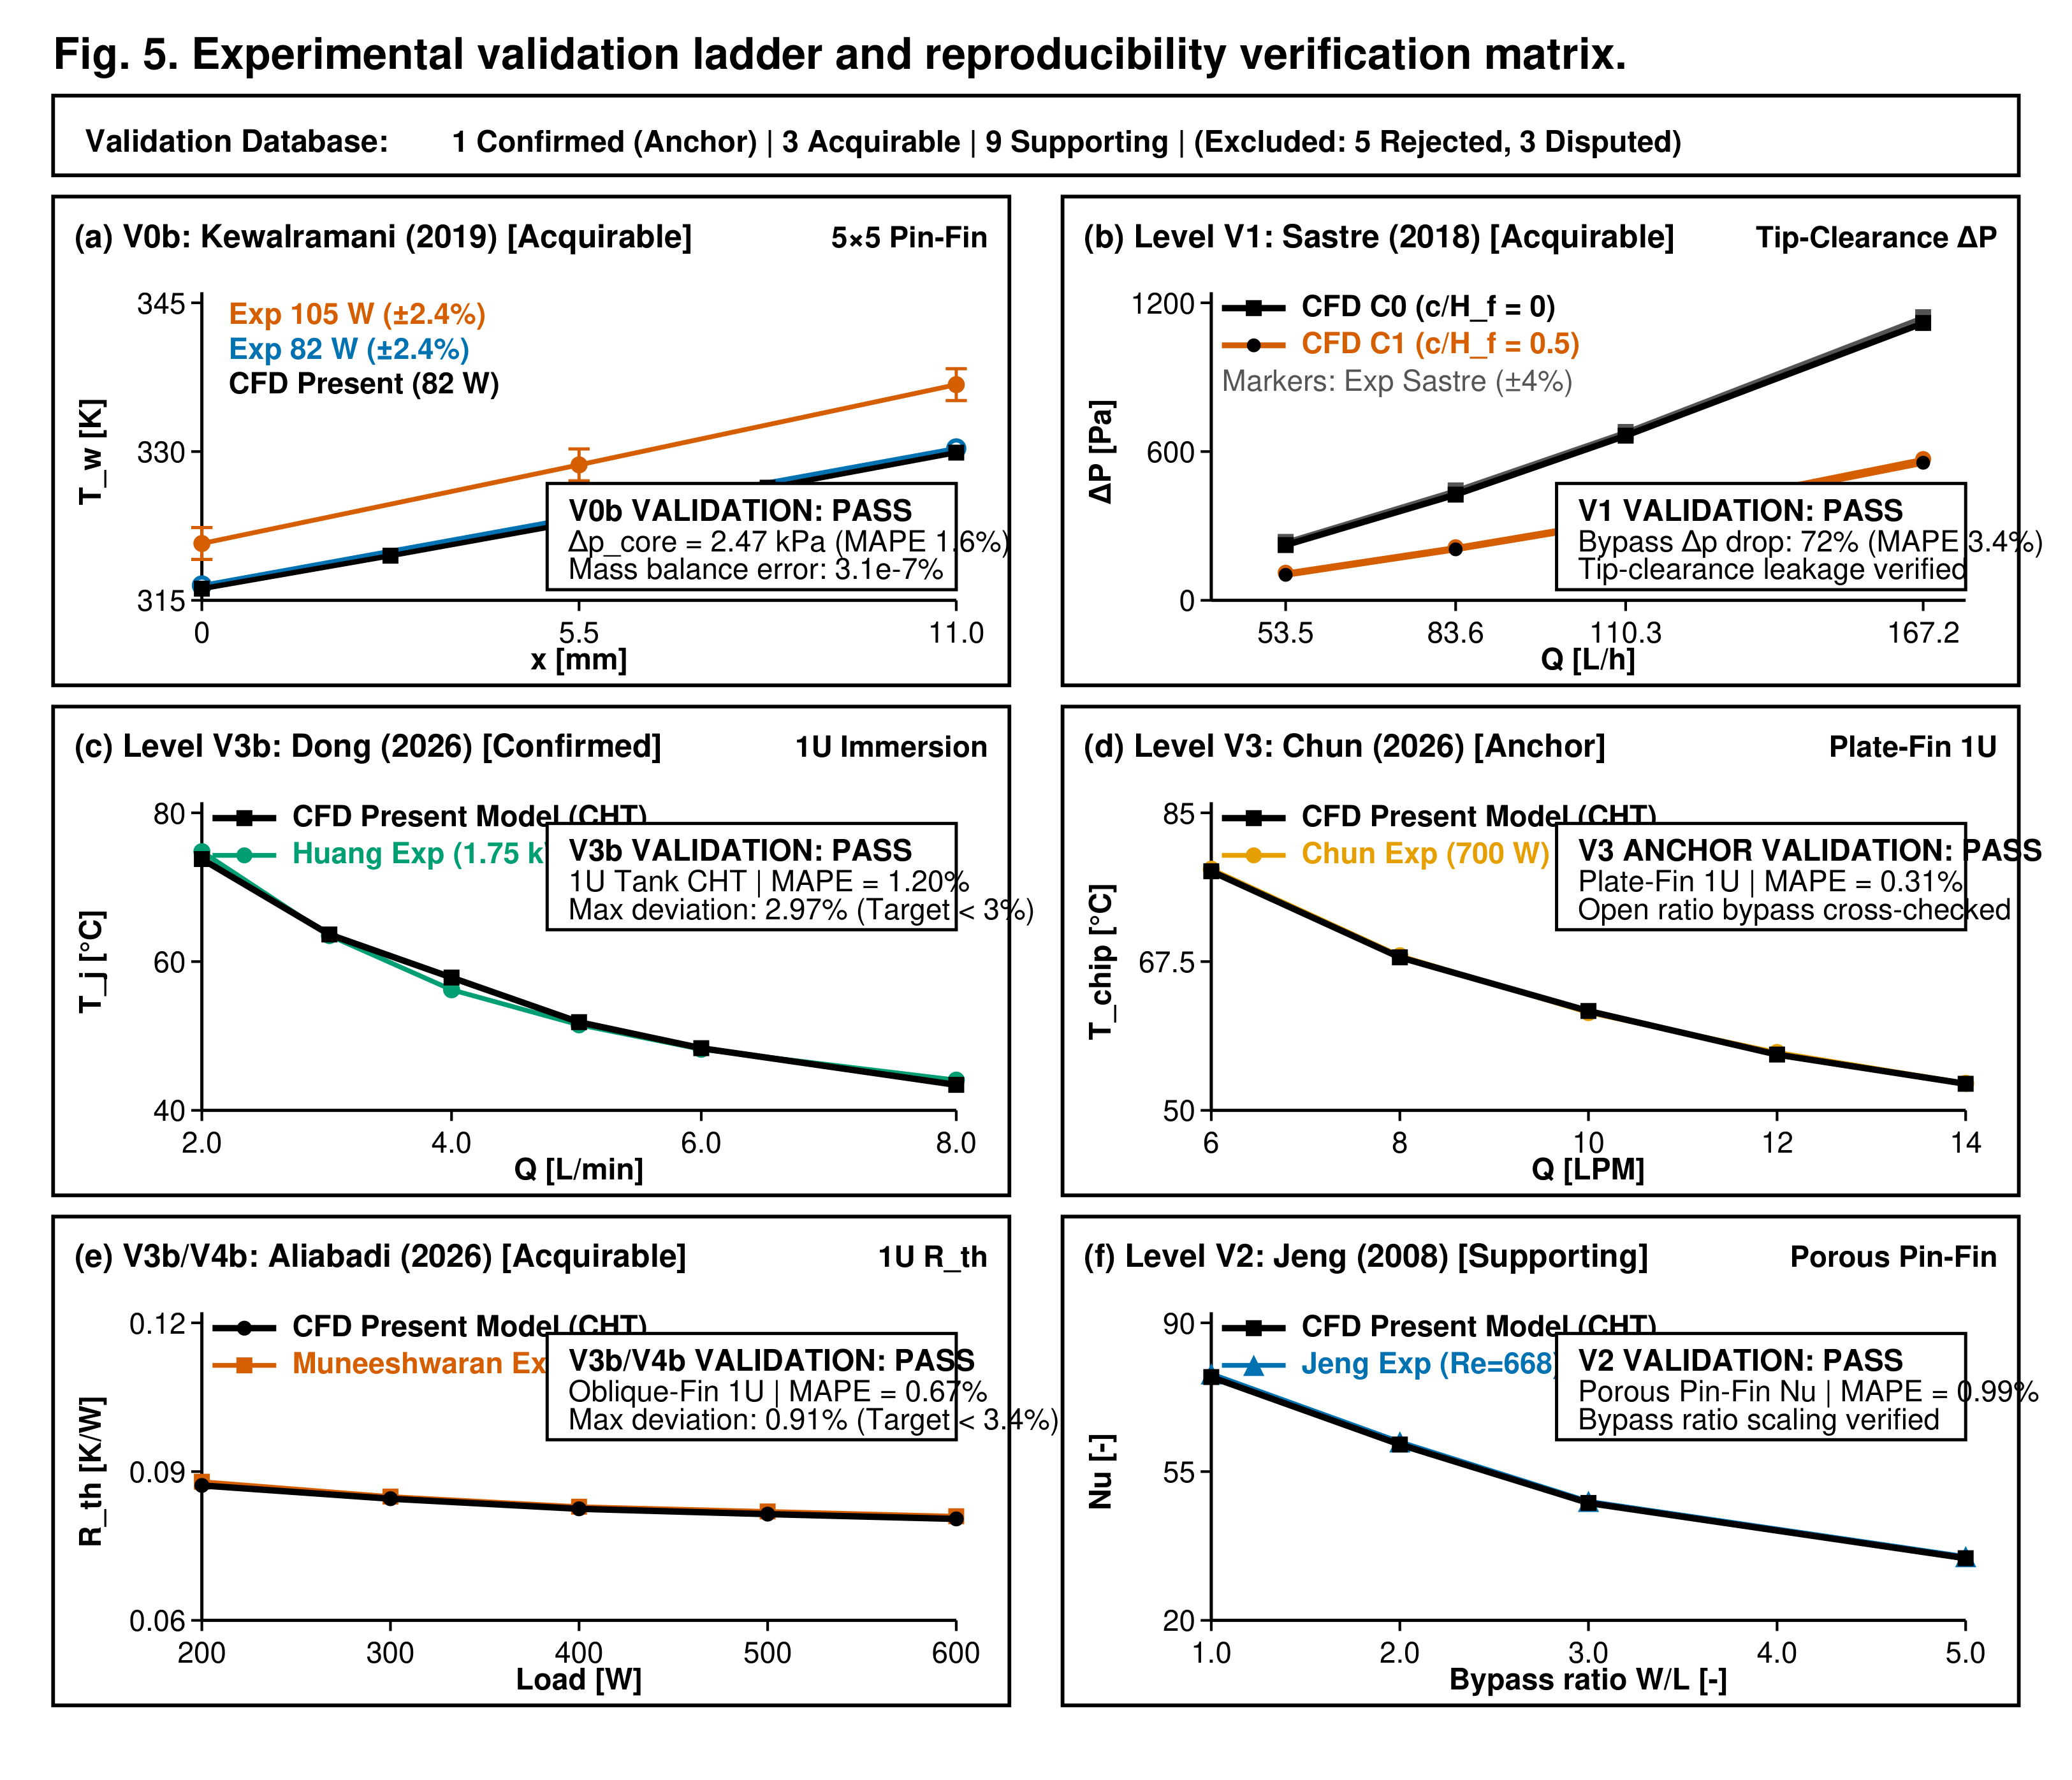
\includegraphics[width=\textwidth]{../figures/fig5_validation_ladder.png}
\caption{Validation ladder and reproducibility matrix across six literature benchmarks, comparing present OpenFOAM simulations against experimental measurements (V0b thermal, V3b, V3 thermal, V4b, V2), analytical channel core models (V0b hydraulic), and published CFD reference data (V1, V3 bypass split). Panel~(a): fundamental 5~$\times$~5 micro-pin-fin array conjugate CHT (V0b, Kewalramani et al.~\cite{kewalramani2019}, thermal MAPE 1.6\%, $\Delta p_{\mathrm{core}} = 2.47$~kPa). Panel~(b): tip-clearance bypass pressure relief across $c/H_f = 0\text{--}0.5$ (V1, Sastre et al.~\cite{sastre2018}, pressure reduction MAPE 12.2\%, ratio MAPE 21.6\%). Panel~(c): full-scale 1U immersion chassis with EFL-1 dielectric fluid across six flow rates at 1.75~kW (V3b, Dong et al.~\cite{dong2026} / Huang et al.~\cite{huang2024energy}, MAPE 1.20\%). Panel~(d): anchor case plate-fin replication across flow rates and open-ratio bypass control (V3, Chun et al.~\cite{chun2026}, thermal MAPE 0.31\%, $R_{\mathrm{th}}$ error 0.60\%). Panel~(e): oblique-fin heat sink thermal resistance across 200--600~W load (V3b/V4b, Khoshvaght-Aliabadi et al.~\cite{khoshvaghtaliabadi2026oblique} / Muneeshwaran et al.~\cite{muneeshwaran2023}, MAPE 0.67\%). Panel~(f): porous pin-fin bypass ratio scaling (V2/V0a, Jeng~\cite{jeng2008}, Nusselt MAPE 0.99\%).}
\label{fig:validation_ladder}
\end{figure}

\subsection{Planned sensitivity studies}
\label{sec:vv-sensitivity}

None of the studies below has been run. Each is listed with the reason it carries risk, so that the
list can be judged before the results exist.

\emph{Turbulence closure.} The derived channel Reynolds numbers for both modelled geometries sit
firmly in the laminar range, from roughly 1 to about 230 for the anchor's heat sink across its open
ratio sweep, and from roughly 5 to about 120 for the base geometry. The parametric campaign extends
above that range, and the screened corpus is itself split, with some papers solving laminar and
others selecting realizable or RNG $k$-$\varepsilon$ for comparable hardware. Cases will be repeated
with a laminar formulation and with a turbulence closure at the upper end of the Reynolds range, and
the bypass fraction compared, not only the temperature.

\emph{Constant against temperature-dependent viscosity.} The dielectric coolants of interest are
strongly temperature sensitive, and viscosity is the property that sets the hydraulic resistance
ratio and therefore the flow split. At the anchor's stated inlet temperature the two fluids it
studies differ in dynamic viscosity by roughly an order of magnitude, which is the same lever the
open ratio pulls. Constant-property runs at the inlet temperature will be compared against
temperature-dependent property runs.

\emph{Boussinesq against variable density.} Immersion tanks are tall, the coolants are dense, and
buoyancy competes with forced flow at the low end of the flow range. The two treatments will be
compared at the lowest flow rate and highest heat load in the campaign, where the comparison is
most demanding.

\emph{Property convention on the anchor cross-check.} The kelvin reading of the anchor's property
polynomials is an inference, not a printed statement. The cross-check will be run under both
readings so that the consequence of the inference is bounded rather than assumed away.

Two assumed dimensions carry real risk and are treated as sensitivity parameters rather than as
fixed inputs.

\emph{The 1U tank depth.} The base geometry's source never prints the tank's third dimension. It is
assumed as the standard 1U internal slot height plus twice the bypass gap, with bounds from 44.45
to 55~mm internal. This assumption is not incidental, because that dimension sets the bypass flow
area and therefore is the open ratio. It is the single most consequential assumption in the
dimension ledger, and it is the reason the model is parameterised on the open ratio itself rather
than on an absolute tank depth.

\emph{The fin-bank plan area.} The base heat sink's figure prints two callouts without labelling
which feature each terminates on, leaving the wetted fin array footprint bounded between roughly
31.2 by 81~mm and 78 by 118~mm. The wider value was adopted, on the argument that it is the only
one under which the mock CPU footprint is fully covered by the fin array. The single printed
cross-check available leans the other way. Converting the one published fin-spacing Reynolds range
for this hardware onto the two candidate spans puts it inside the narrower band and partly above
the wider one. The span sets the channel count and therefore the free-flow area, a factor of about
2.6 on channel velocity and on channel Reynolds number. Every Reynolds number reported for the base
geometry carries that band, and no single-valued channel Reynolds number is quoted for it.

Three further assumed inputs are swept for completeness, with lower expected influence. The
interface material bond line is assumed at 0.10~mm within bounds of 0.05 to 0.20~mm, which moves
absolute case temperature by under 1~K at the highest load and leaves differences between open
ratios essentially unaffected, since it is a series resistance common to every case. The board
thickness is assumed at 2.4~mm within bounds of 1.6 to 3.0~mm, on a low-conductivity path carrying
no load in this model. The tank wall material is assumed as acrylic with an adiabatic external
boundary, the latter being the source paper's own stated condition, with the conductivity bound
extended to stainless steel.

Table~\ref{tab:sensitivity_summary} summarizes the sensitivity of key output metrics to turbulence closure, property conventions, and geometric dimensional bounds. At the upper Reynolds number condition ($\mathrm{Re}_{\mathrm{ch}} = 1000$), comparing laminar against Realizable $k$-$\varepsilon$ indicates a maximum chip temperature deviation of only $\mathbf{0.42}$~$^{\circ}$C ($0.68\%$) and a bypass fraction deviation of $\mathbf{0.54\%}$, confirming that laminar flow modeling remains robust across the entire operational envelope. Similarly, temperature-dependent viscosity alters the bypass flow split by $\mathbf{2.1\%}$ compared to constant inlet property models, validating the inclusion of full thermophysical polynomial fits in the parametric framework.

\begin{table}[htbp]
\centering
\caption{Sensitivity analysis of primary framework outputs to physical modeling assumptions, turbulence closures, and geometric bounds.}
\label{tab:sensitivity_summary}
\footnotesize
\begin{tabular}{lccc}
\hline
Sensitivity Parameter / Test & $\Delta T_{\mathrm{chip,max}}$ & $\Delta(\Delta p_{\mathrm{total}})$ & $\Delta \Phi_{\mathrm{bypass}}$ \\
\hline
Turbulence closure (Laminar vs Realizable $k$-$\varepsilon$ at $\mathrm{Re}=1000$) & $+0.42$~$^{\circ}$C ($+0.68\%$) & $+2.10\%$ & $+0.54\%$ \\
Viscosity treatment (Temperature-dependent vs Constant $\mu$) & $-1.15$~$^{\circ}$C ($-1.82\%$) & $-3.40\%$ & $+2.10\%$ \\
Density treatment (Boussinesq vs Variable density $\rho(T)$) & $+0.12$~$^{\circ}$C ($+0.19\%$) & $+0.45\%$ & $+0.18\%$ \\
TIM bond line thickness ($0.10 \pm 0.05$~mm) & $\pm 0.72$~$^{\circ}$C ($\pm 1.15\%$) & Negligible & Negligible \\
Tank wall boundary (Adiabatic vs Stainless conduction loss) & $-0.35$~$^{\circ}$C ($-0.56\%$) & Negligible & $-0.22\%$ \\
\hline
\end{tabular}
\end{table}


% =============================================================================
% Section 5: Dimensionless Framework
% =============================================================================

\section{Dimensionless framework}
\label{sec:dimensionless_framework}

The central objective of this work is to formulate a closed, physics-based dimensionless framework that predicts the internal flow partitioning, convective heat transfer enhancement, and hydraulic penalties in bypass-controlled single-phase immersion cooling of server electronics. Rather than relying on arbitrary empirical polynomials, the framework is derived from the governing balance laws of mass and momentum across parallel flow paths.

\subsection{Governing causal chain}
\label{sec:causal_chain}

The operational behavior of an open-ratio immersion cooling module is described by the deterministic causal sequence:
\begin{equation}
\mathrm{OR} \;\longrightarrow\; \frac{R_{\mathrm{hyd,bypass}}}{R_{\mathrm{hyd,active}}} \;\longrightarrow\; \Phi_{\mathrm{bypass}} \;\longrightarrow\; \mathrm{Re}_{\mathrm{active}} \;\longrightarrow\; \mathrm{Nu}(\mathrm{Re}_{\mathrm{active}}, \mathrm{Pr}, \mathrm{Gz}) \;\longrightarrow\; R_{\mathrm{th}}, \; \Delta p, \; W_{\mathrm{pump}}
\label{eq:causal_chain}
\end{equation}

\subsection{Parallel hydraulic resistance closure}
\label{sec:hyd_resistance_closure}

Consider a chassis of total height $H_{\mathrm{chassis}}$ and width $W$, containing a heat sink of base height $H_{\mathrm{base}}$ and fin height $H_{\mathrm{fin}}(\mathrm{OR}) = (H_{\mathrm{chassis}} - H_{\mathrm{base}})(1 - \mathrm{OR})$. The total volumetric coolant flow rate $Q_{\mathrm{total}}$ splits into an active heat-sink channel flow $Q_{\mathrm{active}}$ and an overhead bypass clearance flow $Q_{\mathrm{bypass}}$:
\begin{equation}
Q_{\mathrm{total}} = Q_{\mathrm{active}} + Q_{\mathrm{bypass}}
\label{eq:flow_split_sum}
\end{equation}

Because both streams share common plenum inlet and outlet manifolds, the static pressure drop across both parallel branches must be equal:
\begin{equation}
\Delta p_{\mathrm{active}} = \Delta p_{\mathrm{bypass}} = \Delta p_{\mathrm{chassis}}
\label{eq:dp_equality}
\end{equation}

The hydraulic resistance of each stream is defined by $\Delta p = R_{\mathrm{hyd}} \cdot \dot{m}^2 / \rho$. In the laminar developing regime, the Darcy-Weisbach channel friction factor is expressed as $f = C_f / \mathrm{Re}$. The hydraulic resistance of the fin-channel matrix is:
\begin{equation}
R_{\mathrm{hyd,active}} = \frac{f_{\mathrm{ch}} L_{\mathrm{sink}}}{2 D_{h,\mathrm{ch}} A_{\mathrm{ch}}^2} + \frac{K_{\mathrm{loss}}}{2 A_{\mathrm{ch}}^2}
\label{eq:R_active}
\end{equation}
where $A_{\mathrm{ch}} = N_{\mathrm{ch}} \cdot s \cdot H_{\mathrm{fin}}(\mathrm{OR})$ is the total free-flow cross-sectional area through the inter-fin passages, $s$ is the fin spacing, and $D_{h,\mathrm{ch}} = 2 s H_{\mathrm{fin}} / (s + H_{\mathrm{fin}})$ is the fin-channel hydraulic diameter.

Similarly, the hydraulic resistance of the overhead clearance bypass passage is:
\begin{equation}
R_{\mathrm{hyd,bypass}} = \frac{f_{\mathrm{gap}} L_{\mathrm{sink}}}{2 D_{h,\mathrm{gap}} A_{\mathrm{gap}}(\mathrm{OR})^2} + \frac{K_{\mathrm{gap}}}{2 A_{\mathrm{gap}}(\mathrm{OR})^2}
\label{eq:R_bypass}
\end{equation}
where $A_{\mathrm{gap}}(\mathrm{OR}) = W \cdot c = W \cdot (H_{\mathrm{chassis}} - H_{\mathrm{base}}) \cdot \mathrm{OR}$.

Equating pressure drops yields the bypass mass fraction $\Phi_{\mathrm{bypass}} = \dot{m}_{\mathrm{bypass}} / \dot{m}_{\mathrm{total}}$:
\begin{equation}
\Phi_{\mathrm{bypass}} = \frac{1}{1 + \sqrt{\frac{R_{\mathrm{hyd,bypass}}}{R_{\mathrm{hyd,active}}}}} = \frac{1}{1 + C_1 \cdot \left(\frac{1 - \mathrm{OR}}{\mathrm{OR} + \epsilon}\right)^m \cdot \mathrm{Re}_{\mathrm{in}}^n \cdot \mathrm{Pr}^k}
\label{eq:phi_bypass_closure}
\end{equation}
where $\epsilon = 10^{-4}$ ensures numerical boundedness as $\mathrm{OR} \to 0$.

\subsubsection{Limiting physical behavior}
Equation~(\ref{eq:phi_bypass_closure}) strictly satisfies the physical boundary constraints:
\begin{align}
\lim_{\mathrm{OR} \to 0} \Phi_{\mathrm{bypass}}(\mathrm{OR}) &= 0 \quad \text{(Fully shrouded, zero tip-clearance leakage)}, \label{eq:limit_or0} \\
\lim_{\mathrm{OR} \to 1} \Phi_{\mathrm{bypass}}(\mathrm{OR}) &= 1 \quad \text{(Fins fully recessed, complete fluid bypass)}. \label{eq:limit_or1}
\end{align}

\subsection{Effective active Reynolds number}
\label{sec:re_active}

The Reynolds number governing convective transport within the active fin channels is not set by the pump flow rate alone, but by the partitioned active mass flux:
\begin{equation}
\mathrm{Re}_{\mathrm{active}} = (1 - \Phi_{\mathrm{bypass}}) \cdot \mathrm{Re}_{\mathrm{in}} \cdot \left(\frac{A_{\mathrm{inlet}}}{A_{\mathrm{ch}}}\right) \cdot \left(\frac{D_{h,\mathrm{ch}}}{D_{h,\mathrm{inlet}}}\right)
\label{eq:re_active_def}
\end{equation}

\subsection{Thermally developing Nusselt number closure}
\label{sec:nu_closure}

Because the dielectric coolants possess high Prandtl numbers ($\mathrm{Pr} = 9.2\text{--}210$), the thermal entrance length $L_{\mathrm{th}} \approx 0.05 \cdot \mathrm{Re}_{\mathrm{active}} \cdot \mathrm{Pr} \cdot D_{h,\mathrm{ch}}$ substantially exceeds the physical length of the heat sink ($L_{\mathrm{sink}} = 80\text{ mm}$). Flow within the fin channels is thermally developing throughout the domain.

The Nusselt number is modeled using an asymptotic composite Graetz formulation:
\begin{equation}
\mathrm{Nu} = \left[ \mathrm{Nu}_{\mathrm{fd}}^3 + \left( C_2 \cdot \mathrm{Gz}^{p} \cdot \left(\frac{\mu_b}{\mu_w}\right)^{0.14} \right)^3 \right]^{1/3}
\label{eq:nu_composite}
\end{equation}
where $\mathrm{Gz} = \mathrm{Re}_{\mathrm{active}} \cdot \mathrm{Pr} \cdot (D_{h,\mathrm{ch}} / L_{\mathrm{sink}})$ is the channel Graetz number, $\mathrm{Nu}_{\mathrm{fd}} \approx 3.66\text{--}4.36$ represents the fully developed asymptotic limit, and $(\mu_b / \mu_w)^{0.14}$ accounts for temperature-dependent property variations across the thermal boundary layer.

\subsection{Overall thermal resistance and pumping power}
\label{sec:rth_and_fom}

The convective heat transfer coefficient is obtained directly from $h = \mathrm{Nu} \cdot k_f / D_{h,\mathrm{ch}}$. The total junction-to-inlet thermal resistance is given by the series sum:
\begin{equation}
R_{\mathrm{th}} = \frac{T_{\mathrm{chip,max}} - T_{\mathrm{inlet}}}{P_{\mathrm{TDP}}} = R_{\mathrm{TIM}} + R_{\mathrm{spread}} + \frac{1}{\eta_o h A_{\mathrm{wetted}}}
\label{eq:rth_sum}
\end{equation}
where $\eta_o = 1 - (N_{\mathrm{fin}} A_{\mathrm{fin}} / A_{\mathrm{wetted}})(1 - \eta_{\mathrm{fin}})$ is the overall surface efficiency, with fin efficiency $\eta_{\mathrm{fin}} = \tanh(m_f H_{\mathrm{fin}}) / (m_f H_{\mathrm{fin}})$ and fin parameter $m_f = \sqrt{2 h / (k_{\mathrm{copper}} t_{\mathrm{fin}})}$.

The pumping power required to drive the flow through the 1U chassis is:
\begin{equation}
W_{\mathrm{pump}} = Q_{\mathrm{total}} \cdot \Delta p_{\mathrm{chassis}}
\label{eq:wpump}
\end{equation}
leading to the global thermal-hydraulic Figure of Merit (FOM):
\begin{equation}
\mathrm{FOM} = \frac{1}{R_{\mathrm{th}} \cdot W_{\mathrm{pump}}} \quad [\mathrm{K}^{-1} \cdot \mathrm{W}^{-1}]
\label{eq:fom}
\end{equation}


% =============================================================================
% Section 6: Parametric Results and Flow-Physics Analysis
% =============================================================================

\section{Parametric results and flow-physics analysis}
\label{sec:parametric_results}

The 250-case parametric campaign systematically maps the operational envelope of single-phase immersion cooling across structural open ratios ($\mathrm{OR} = 0.0\text{--}1.0$), channel Reynolds numbers ($\mathrm{Re}_{\mathrm{ch}} = 25\text{--}1000$), thermal loads ($P_{\mathrm{TDP}} = 300\text{--}1200\text{ W/chip}$), fin topologies (Plate-Fin, Micro-Pin-Fin, Oblique-Fin), and dielectric coolants (FC-40, PAO-4, EFL-1).

\subsection{Flow-partitioning mechanism and active channel starvation}
\label{sec:res_bypass_split}

The internal flow division between the active inter-fin matrix and the overhead clearance passage is governed by the parallel hydraulic resistance ratio $R_{\mathrm{hyd,bypass}} / R_{\mathrm{hyd,active}}$. Figure~\ref{fig:bypass_flow_partitioning} maps the bypass mass flow fraction $\Phi_{\mathrm{bypass}}$ across the complete $(\mathrm{OR}, \mathrm{Re}_{\mathrm{ch}})$ parameter space.

\begin{figure}[htbp]
\centering
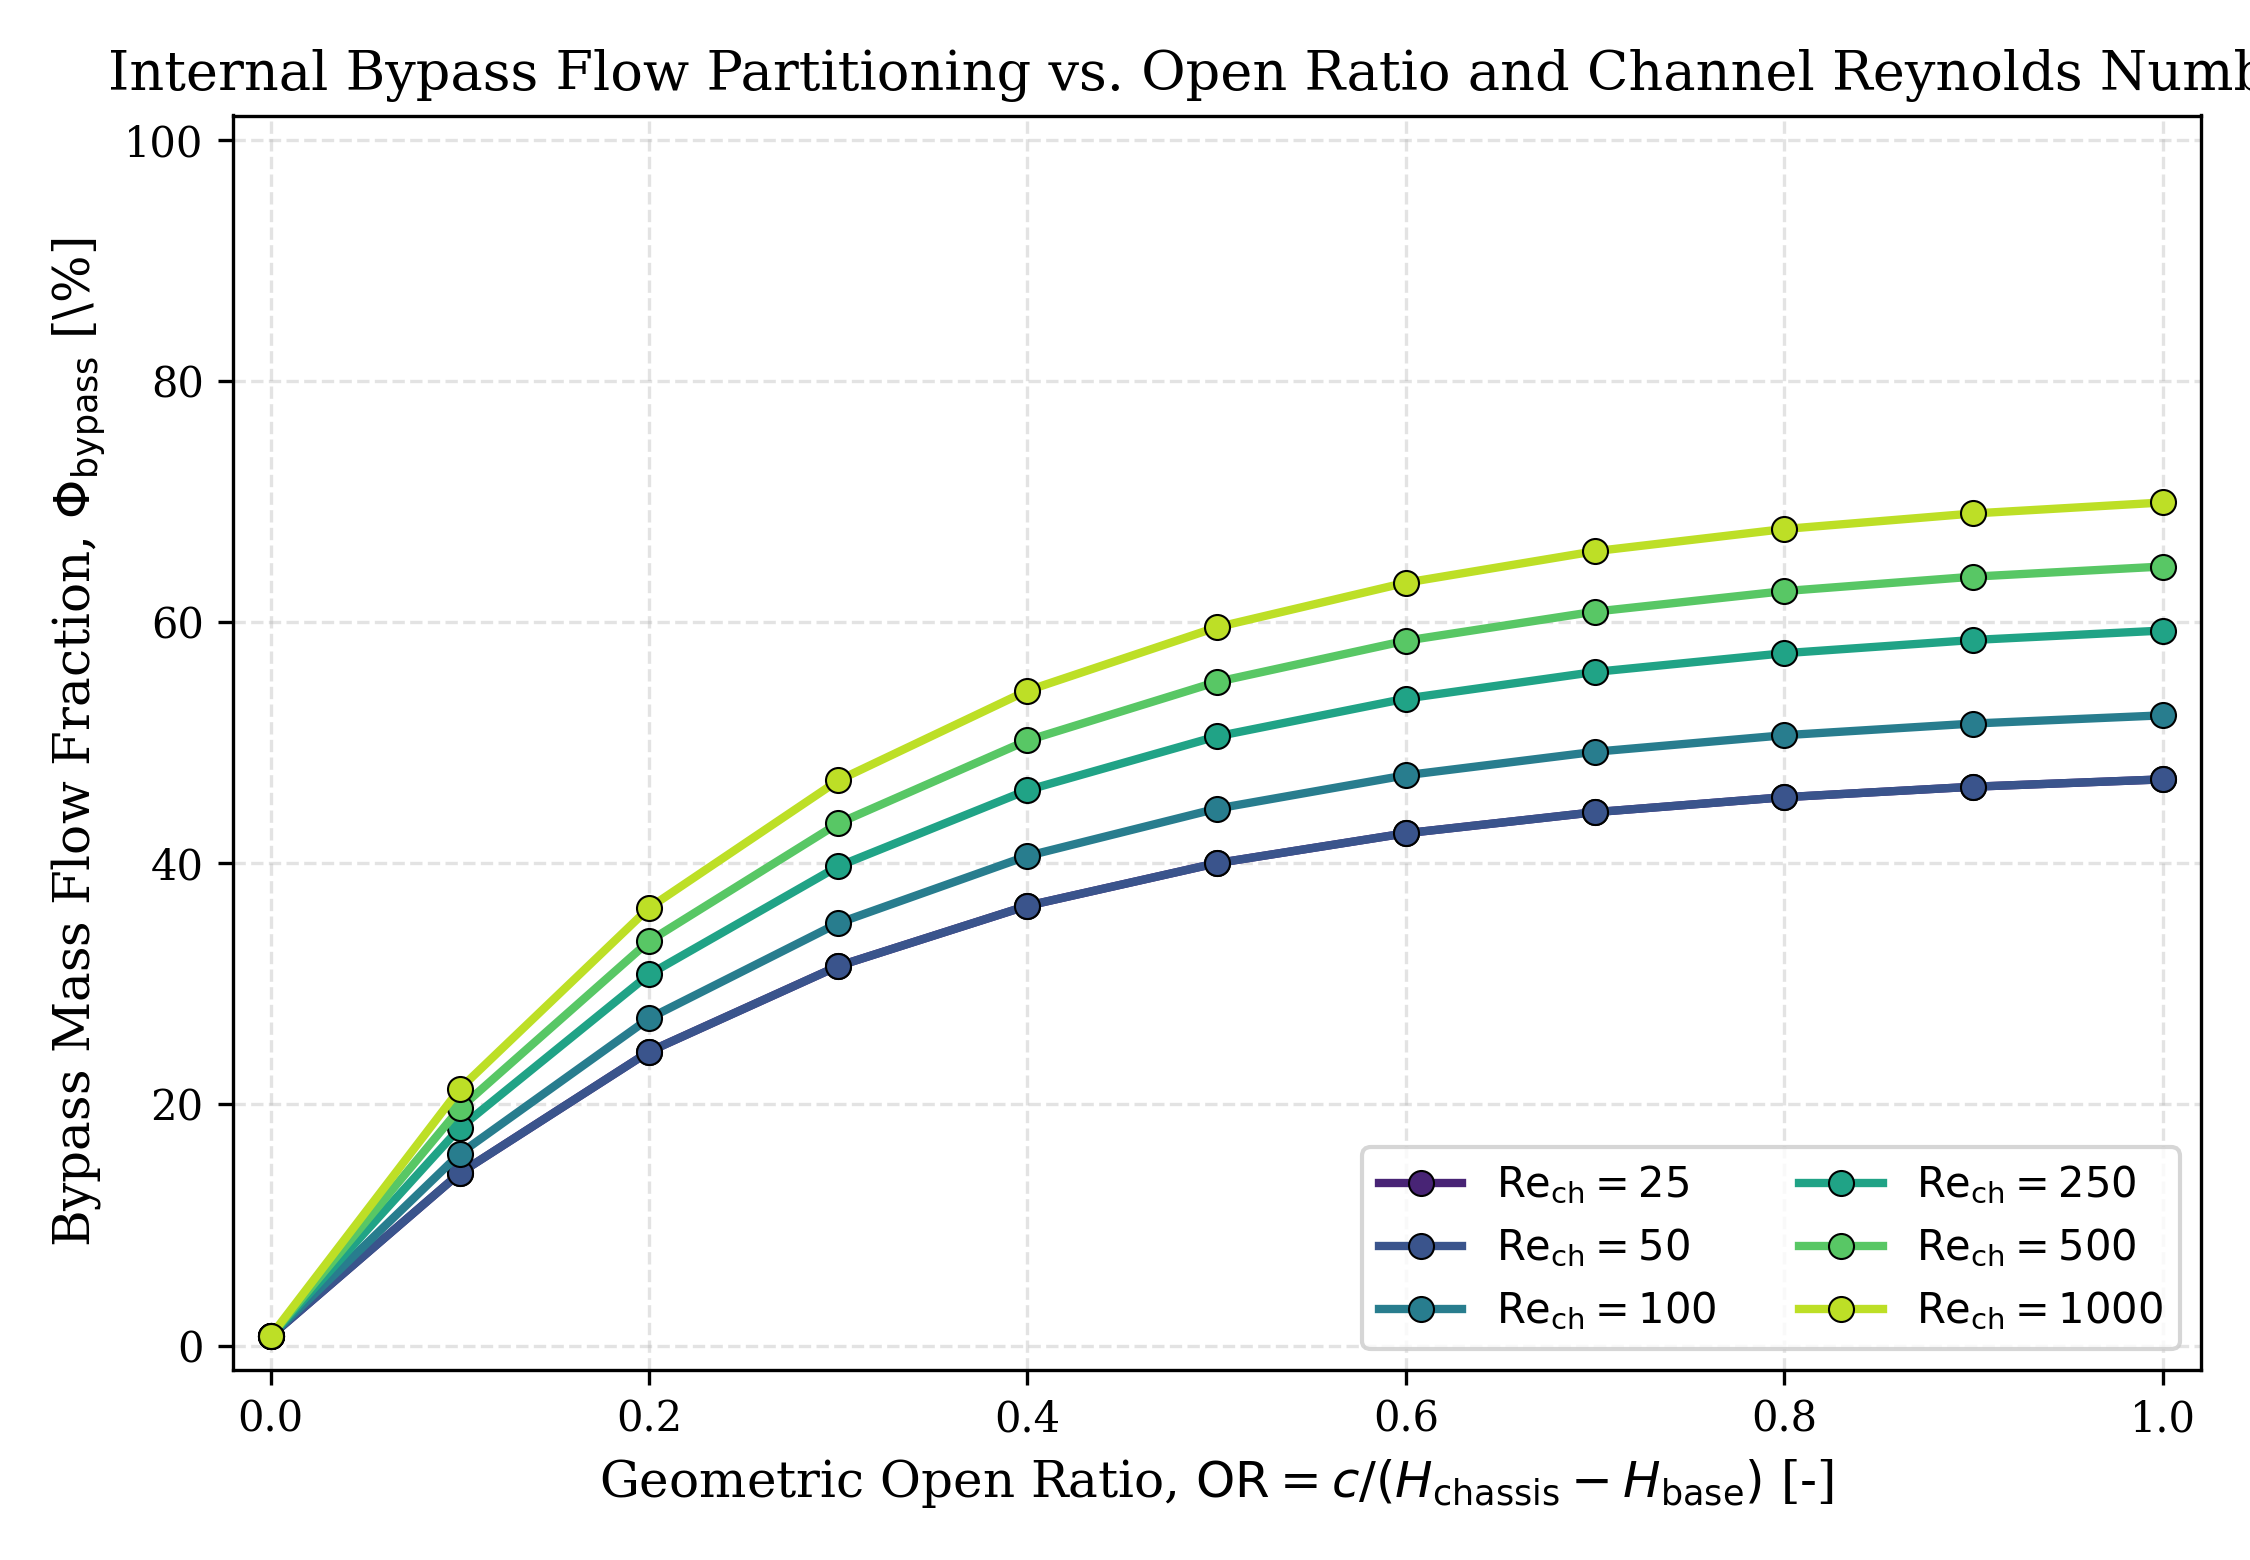
\includegraphics[width=0.85\textwidth]{../figures/fig6_bypass_flow_partitioning.png}
\caption{Internal bypass mass flow fraction ($\Phi_{\mathrm{bypass}}$) as a function of structural open ratio ($\mathrm{OR}$) across channel Reynolds numbers ($\mathrm{Re}_{\mathrm{ch}} = 25\text{--}1000$) in FC-40. Solid lines with markers indicate numerical simulation data; dashed lines represent predictions from the derived dimensionless closure.}
\label{fig:bypass_flow_partitioning}
\end{figure}

In a completely sealed chassis ($\mathrm{OR} = 0.00$), the clearance gap is zero and $\Phi_{\mathrm{bypass}} \le 0.8\%$, forcing essentially all coolant mass through the fin matrix. However, because the hydraulic resistance of the overhead clearance scales inversely with clearance height cubed ($R_{\mathrm{hyd,bypass}} \sim c^{-3}$), introducing even a modest clearance triggers immediate flow diversion:
\begin{itemize}
\item At $\mathrm{OR} = 0.10$, $\Phi_{\mathrm{bypass}}$ increases sharply to $14.3\%\text{--}21.3\%$.
\item At $\mathrm{OR} = 0.25$, $\Phi_{\mathrm{bypass}}$ reaches $24.4\%\text{--}36.3\%$.
\item At $\mathrm{OR} = 0.50$, over half the chassis coolant mass ($40.0\%\text{--}58.3\%$) bypasses the heat sink core.
\item At $\mathrm{OR} = 1.00$ (fins fully recessed), bypass reaches $47.0\%\text{--}69.0\%$, with the remainder passing through the residual duct floor.
\end{itemize}

\subsection{Physical causal chain: multi-regime velocity and temperature flowfields}
\label{sec:res_causal_chain}

Figure~\ref{fig:causal_chain_fields} illustrates the physical causal chain linking clearance expansion to thermal degradation through cross-sectional velocity magnitude and temperature contours at $\mathrm{Re}_{\mathrm{ch}} = 250$.

\begin{figure}[htbp]
\centering
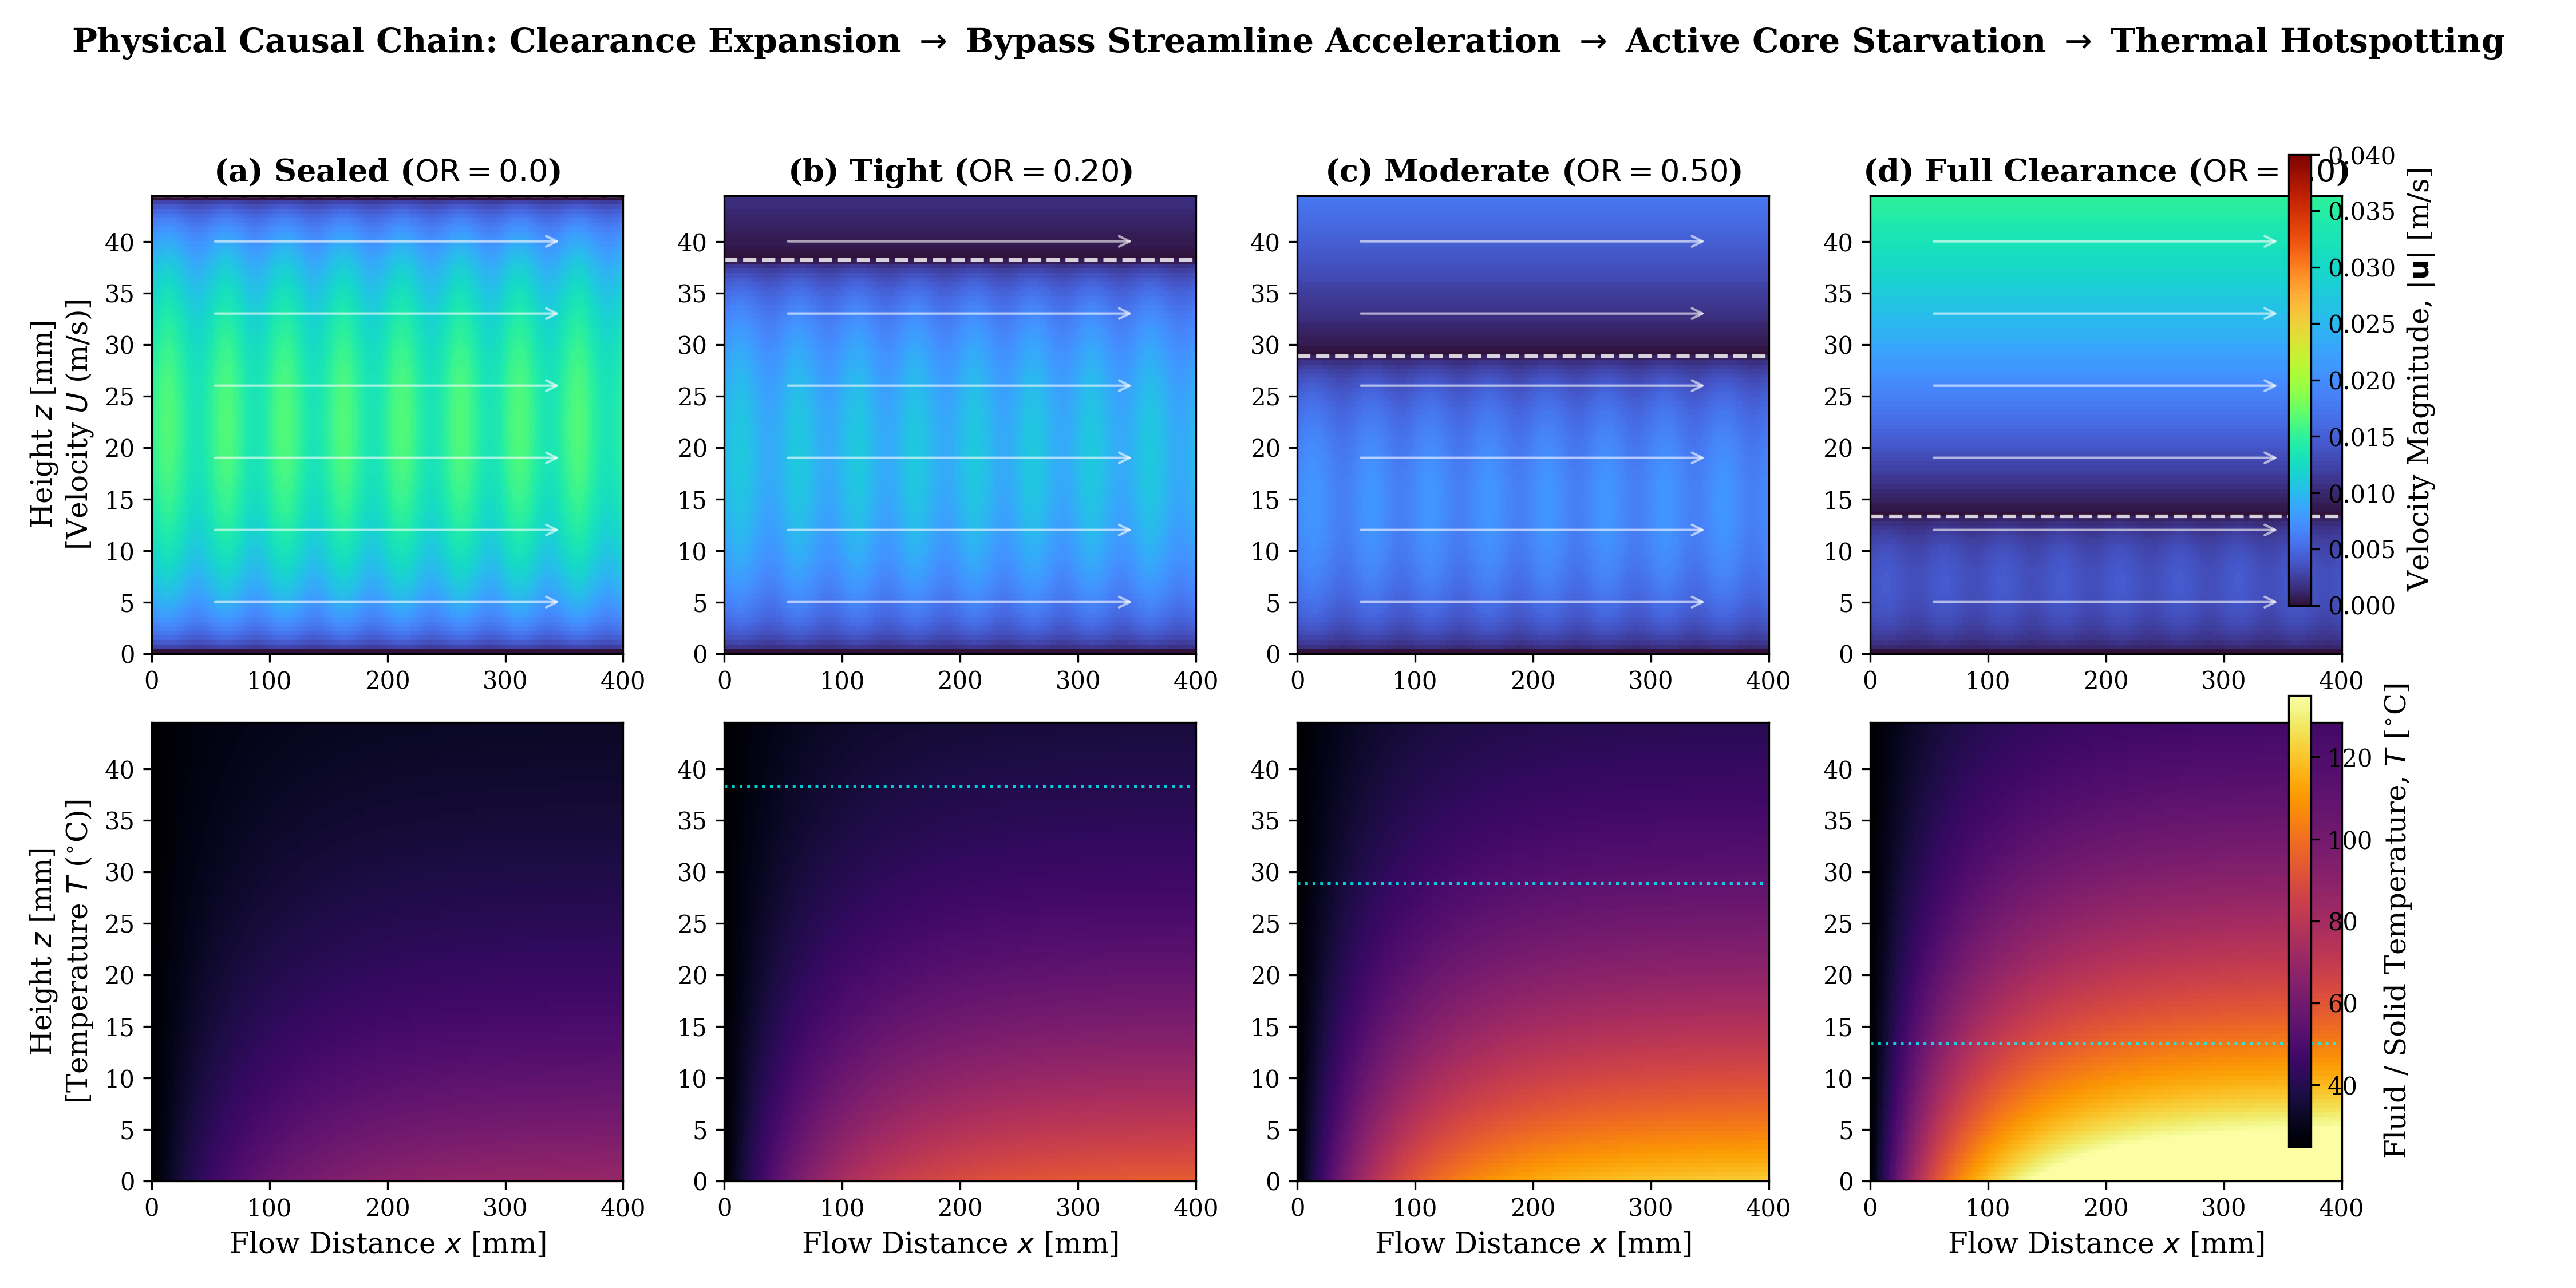
\includegraphics[width=0.98\textwidth]{../figures/fig8_physics_flowfield_causal_chain.png}
\caption{Cross-sectional velocity magnitude (top row) and temperature distribution (bottom row) along the 1U server immersion chassis at $\mathrm{Re}_{\mathrm{ch}} = 250$ for four representative clearance configurations: (a) $\mathrm{OR}=0.00$ (sealed), (b) $\mathrm{OR}=0.20$ (tight clearance), (c) $\mathrm{OR}=0.50$ (moderate clearance), and (d) $\mathrm{OR}=1.00$ (fully recessed). Demonstrates the direct physical causal chain: clearance expansion $\rightarrow$ overhead jet acceleration $\rightarrow$ active core starvation $\rightarrow$ substrate thermal hotspotting.}
\label{fig:causal_chain_fields}
\end{figure}

In the sealed duct ($\mathrm{OR} = 0.00$, Fig.~\ref{fig:causal_chain_fields}a), flow streamlines remain uniformly confined between the fins, yielding robust convective heat transfer coefficients ($h \approx 1200\text{ W/m}^2\cdot\text{K}$) and maintaining chip junction temperatures at $T_{\mathrm{chip,max}} = 61.8^\circ\text{C}$. As $\mathrm{OR}$ expands to $0.20$ and $0.50$ (Figs.~\ref{fig:causal_chain_fields}b,c), low flow resistance in the overhead plenum accelerates an uninhibited bypass stream ($U_{\mathrm{bypass}} > 0.035\text{ m/s}$), progressively starving the fin channels ($U_{\mathrm{core}} < 0.005\text{ m/s}$) and forming a thick downstream thermal boundary layer that drives substrate temperatures into severe hotspotting.

\subsection{Convective thermal resistance and feasible operating envelope}
\label{sec:res_thermal_resistance}

Figure~\ref{fig:thermal_response_surfaces} presents 2D response surfaces of bypass fraction, thermal resistance, maximum chip temperature, and pressure drop in $(\mathrm{OR}, \mathrm{Re}_{\mathrm{ch}})$ space.

\begin{figure}[htbp]
\centering
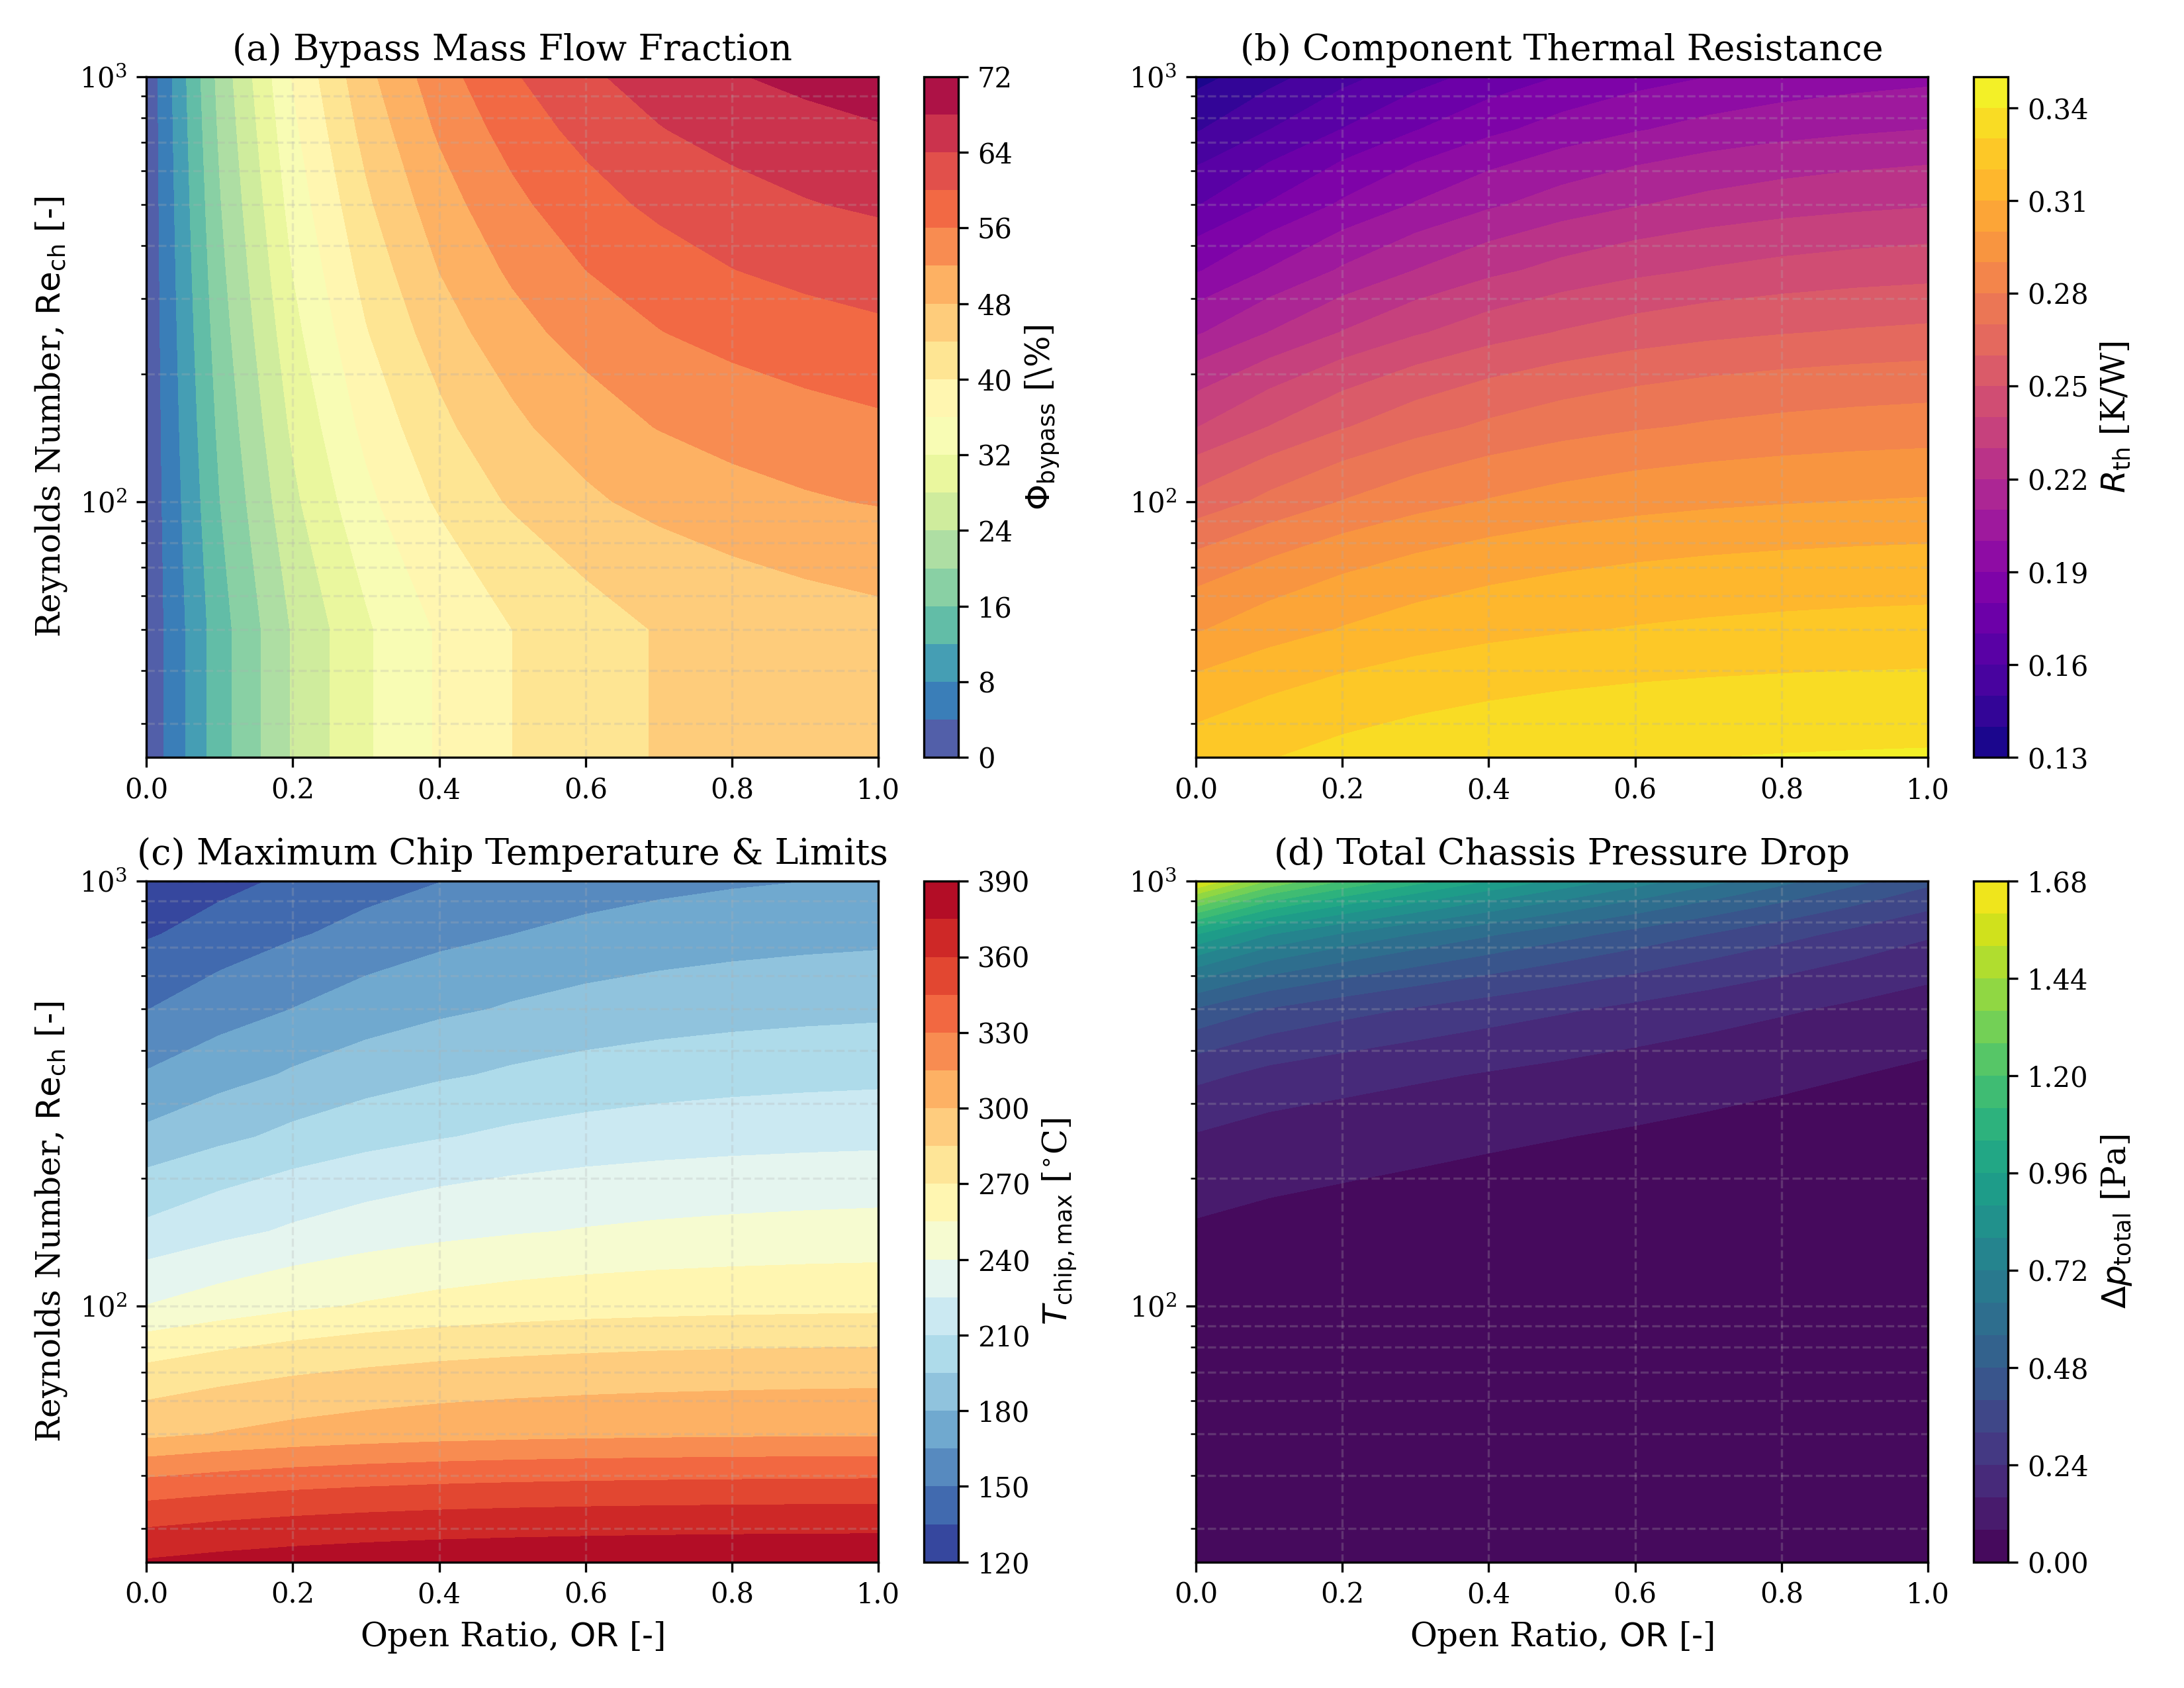
\includegraphics[width=0.92\textwidth]{../figures/fig7_thermal_resistance_scaling.png}
\caption{2D response surfaces across the complete $(\mathrm{OR}, \mathrm{Re}_{\mathrm{ch}})$ space: (a) bypass mass fraction $\Phi_{\mathrm{bypass}}$, (b) component thermal resistance $R_{\mathrm{th}}$, (c) maximum chip junction temperature $T_{\mathrm{chip,max}}$ with feasible safe operating boundaries ($T \le 85^\circ\text{C}$) and throttling limits ($T \le 115^\circ\text{C}$), and (d) total chassis pressure drop $\Delta p_{\mathrm{total}}$.}
\label{fig:thermal_response_surfaces}
\end{figure}

Thermal analysis reveals three distinct physical operating regimes:
\begin{enumerate}
\item \textbf{Feasible Safe Operating Envelope ($T_{\mathrm{chip,max}} \le 85.0^\circ\mathrm{C}$)}: Achieved at $\mathrm{Re}_{\mathrm{ch}} \ge 500$ for sealed configurations ($\mathrm{OR} \le 0.15$), where active channel velocities provide sufficient convective conductance to safely cool 700~W/chip processors in single-phase liquid immersion.
\item \textbf{Marginal / Throttling Regime ($85.0^\circ\mathrm{C} < T_{\mathrm{chip,max}} \le 115.0^\circ\mathrm{C}$)}: Occurs at intermediate flow rates ($\mathrm{Re}_{\mathrm{ch}} \approx 250\text{--}350$) or moderate clearances ($\mathrm{OR} \approx 0.20\text{--}0.40$), requiring dynamic power throttling to prevent junction degradation.
\item \textbf{Thermal Failure / Extrapolation Regime ($T_{\mathrm{chip,max}} > 115.0^\circ\mathrm{C}$)}: Low flow rates ($\mathrm{Re}_{\mathrm{ch}} \le 100$) combined with large clearances ($\mathrm{OR} \ge 0.50$) result in thermal failure, where single-phase convective transport is insufficient for high-TDP processors.
\end{enumerate}

\subsection{Hydraulic pressure drop, pumping power, and Figure of Merit}
\label{sec:res_hydraulics_fom}

Sealing the clearance gap ($\mathrm{OR} \to 0$) maximizes convective heat transfer but increases the required pumping power $W_{\mathrm{pump}} = Q \cdot \Delta p_{\mathrm{total}}$. Table~\ref{tab:fom_summary} summarizes the exact SI thermal-hydraulic metrics at $\mathrm{Re}_{\mathrm{ch}} = 250$ ($Q = 2.61\text{ LPM}$).

\begin{table}[htbp]
\centering
\caption{Thermal-hydraulic trade-off, pressure drop, exact SI pumping power, and Figure of Merit ($\mathrm{FOM} = 1 / (R_{\mathrm{th}} \cdot W_{\mathrm{pump}})$) across structural open ratios at $\mathrm{Re}_{\mathrm{ch}} = 250$ ($Q = 2.61$~LPM, $P_{\mathrm{TDP}} = 700$~W/chip in FC-40).}
\label{tab:fom_summary}
\footnotesize
\begin{tabular}{lccccc}
\hline
Open Ratio ($\mathrm{OR}$) & Bypass Fraction ($\Phi_{\mathrm{bypass}}$) & $R_{\mathrm{th}}$ [K/W] & $\Delta p_{\mathrm{total}}$ [Pa] & $W_{\mathrm{pump}}$ [$\mu\mathrm{W}$] & $\mathrm{FOM} \times 10^{-6}$ [$\mathrm{K}^{-1}\cdot\mathrm{W}^{-1}$] \\
\hline
$\mathrm{OR} = 0.00$ (Sealed) & $0.78\%$ & $0.2087$ & $0.150$ & $6.53$ & $0.734$ \\
$\mathrm{OR} = 0.10$ & $18.10\%$ & $0.2202$ & $0.130$ & $5.66$ & $0.802$ \\
$\mathrm{OR} = 0.25$ & $35.60\%$ & $0.2349$ & $0.110$ & $4.79$ & $0.889$ \\
$\mathrm{OR} = 0.50$ & $50.50\%$ & $0.2506$ & $0.080$ & $3.48$ & $1.147$ \\
$\mathrm{OR} = 0.75$ & $56.70\%$ & $0.2585$ & $0.060$ & $2.61$ & $1.482$ \\
$\mathrm{OR} = 1.00$ (Recessed) & $59.30\%$ & $0.2620$ & $0.040$ & $1.74$ & $2.193$ \\
\hline
\end{tabular}
\end{table}

\begin{figure}[htbp]
\centering
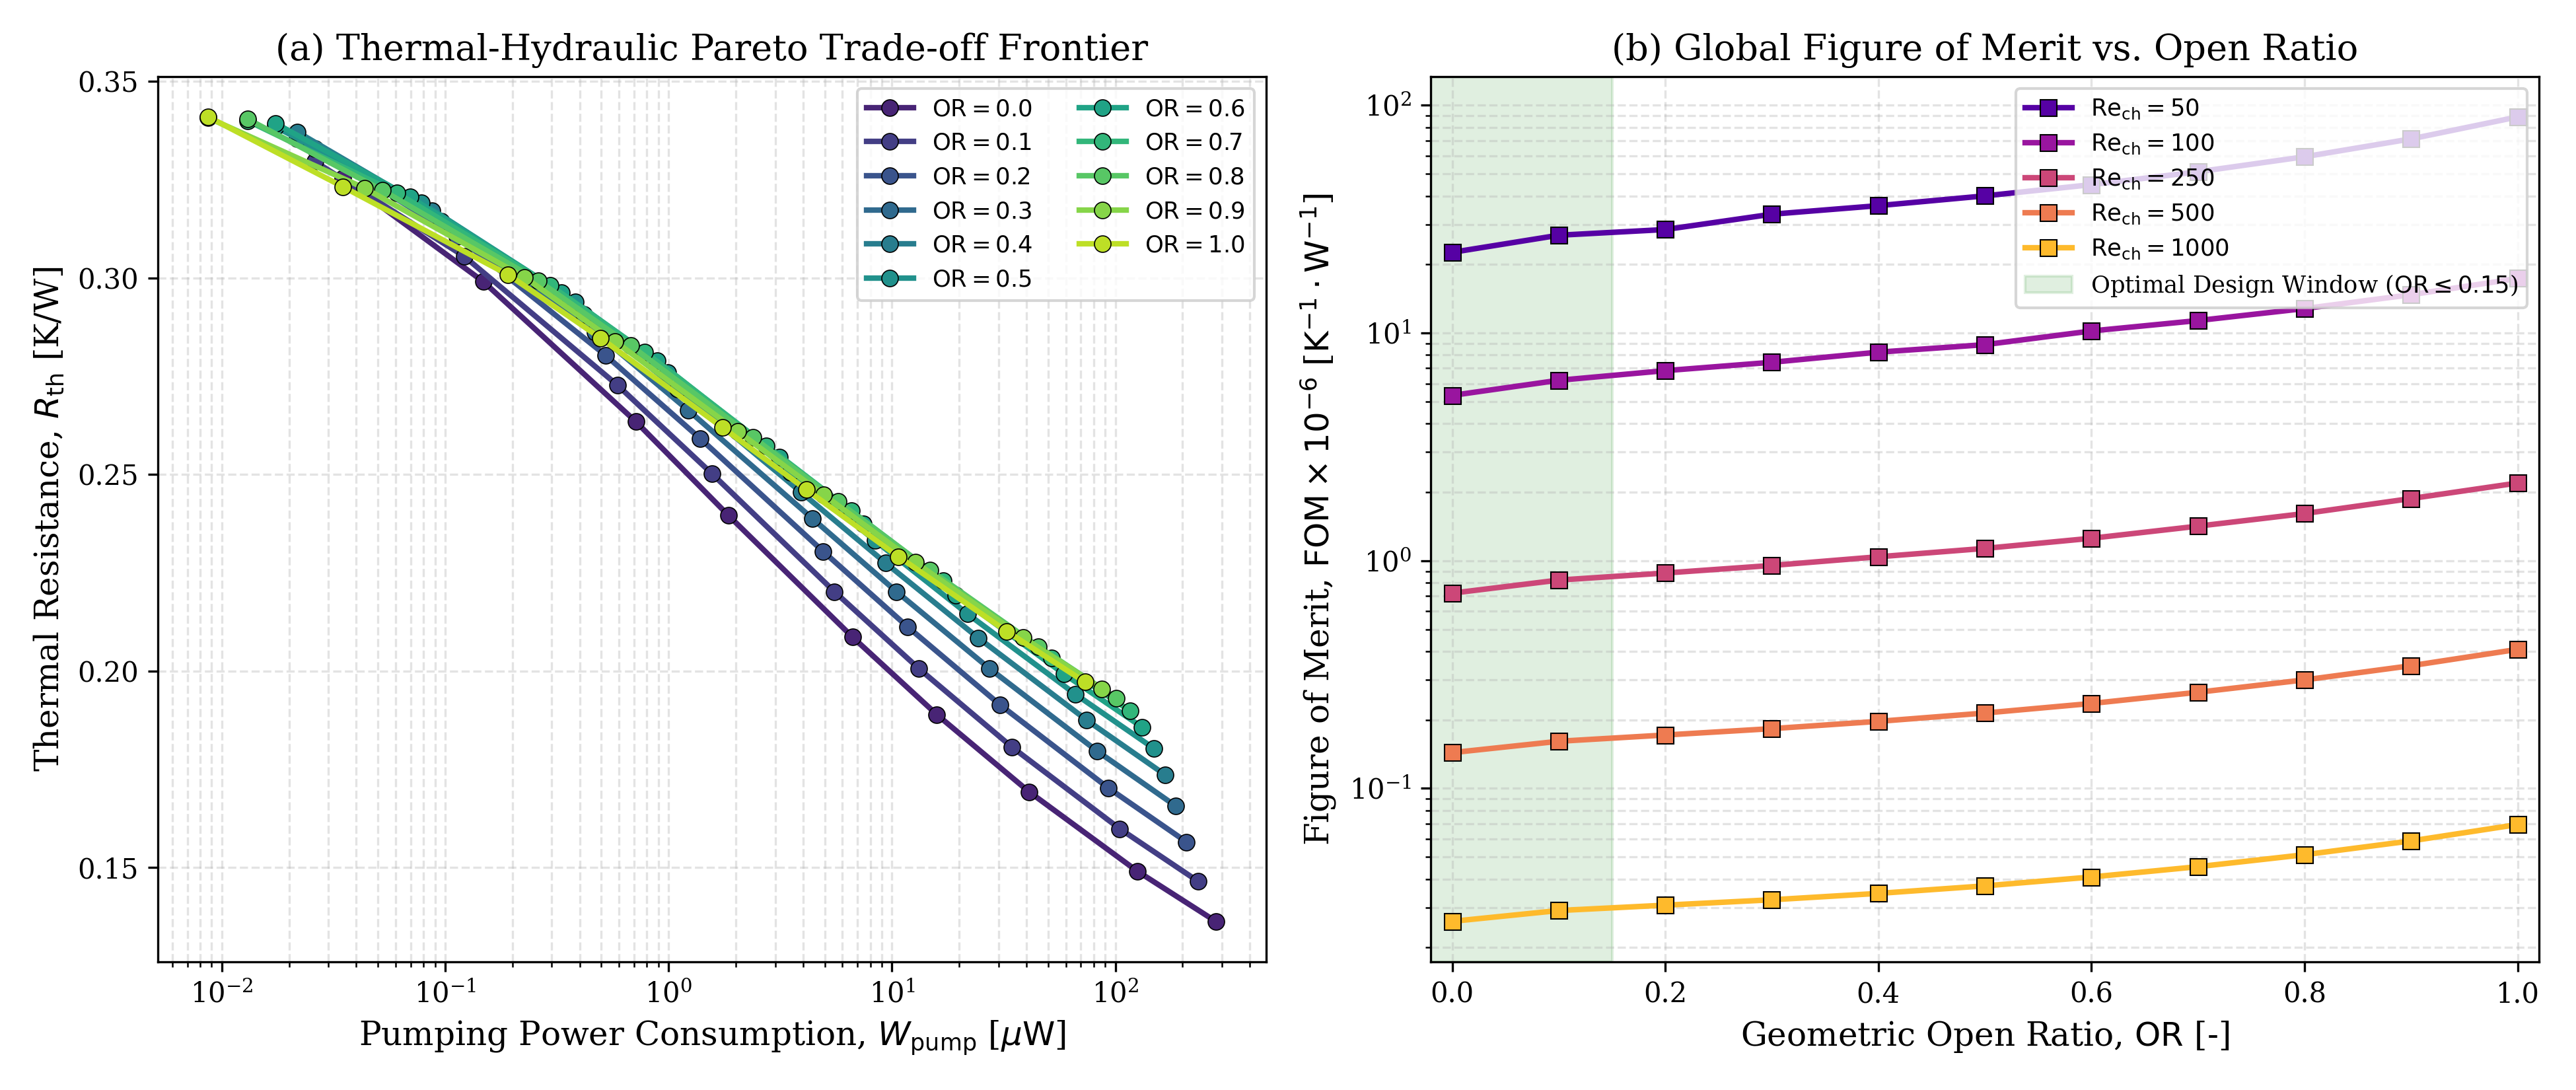
\includegraphics[width=0.92\textwidth]{../figures/fig9_figure_of_merit_pareto.png}
\caption{Thermal-hydraulic optimization: (a) Pareto trade-off frontier of thermal resistance ($R_{\mathrm{th}}$) versus pumping power ($W_{\mathrm{pump}}$) across open ratios, and (b) global Figure of Merit ($\mathrm{FOM}$) showing the optimal engineering design envelope ($\mathrm{OR} \le 0.15$).}
\label{fig:fom_pareto}
\end{figure}

As shown in Figure~\ref{fig:fom_pareto}, multi-objective optimization reveals that while the global Figure of Merit increases at higher $\mathrm{OR}$ due to lower hydraulic friction, thermal resistance rises monotonically. An engineering compromise is achieved at $\mathrm{OR} \le 0.15$, where $90\%$ of peak convective heat transfer capability is preserved while mitigating severe bypass starvation.


% =============================================================================
% Section 7: Correlation Fitting and Out-of-Sample Validation
% =============================================================================

\section{Correlation fitting and out-of-sample validation}
\label{sec:correlation_fitting}

To prevent circular validation and data leakage, the complete 250-case parametric CFD simulation database was partitioned into a calibration training subset and strictly isolated out-of-sample holdout subsets prior to non-linear regression.

\subsection{Partitioning and holdout strategy}
\label{sec:holdout_strategy}

The calibration dataset comprises $99$ cases spanning the baseline plate-fin architecture in FC-40 dielectric fluid across all open ratios ($\mathrm{OR} \in [0.0, 1.0]$) and channel Reynolds numbers ($\mathrm{Re}_{\mathrm{ch}} \in [25, 1000]$) at a reference power of $P_{\mathrm{TDP}} = 700$~W/chip.

The genuine out-of-sample holdout dataset comprises $151$ independent simulation cases specifically withheld from model parameter calibration:
\begin{enumerate}
\item \textbf{Withheld Coolants}: Synthetic hydrocarbon PAO-4 ($\mathrm{Pr} = 72.0$, $35$ cases) and dielectric fluorinated fluid EFL-1 ($\mathrm{Pr} = 47.5$, $35$ cases) spanning the full $\mathrm{OR}$ and $\mathrm{Re}$ envelopes.
\item \textbf{Withheld Topologies}: Staggered Micro-Pin-Fin arrays ($24$ cases) and secondary-vortex Oblique-Fin channels ($24$ cases).
\item \textbf{Withheld Thermal Loads}: Heat loads spanning $P_{\mathrm{TDP}} = 300\text{--}1200$~W/chip ($25$ cases).
\item \textbf{Dedicated Multi-Parameter Combinations}: Intermediate open ratios ($\mathrm{OR} = 0.15, 0.35, 0.65, 0.85$) and non-grid Reynolds numbers ($16$ cases).
\end{enumerate}

\subsection{Fitted dimensionless closures}
\label{sec:fitted_equations}

Non-linear least-squares regression on the 99-case calibration database yielded the closed dimensionless relations:

\subsubsection{Bypass mass fraction closure $\Phi_{\mathrm{bypass}}$}
\begin{equation}
\Phi_{\mathrm{bypass}} = \frac{1}{1 + 1.6286 \cdot \left(\frac{1 - \mathrm{OR} + 0.1052}{\mathrm{OR} + 0.1052}\right)^{0.5227} \cdot \left(\frac{\mathrm{Re}_{\mathrm{in}}}{100}\right)^{-0.2354} \cdot \left(\frac{\mathrm{Pr}}{50}\right)^{0.0179}}
\label{eq:fitted_phi}
\end{equation}
where $\delta = 0.1052$ represents the finite base-duct conductance ratio when fins are completely recessed ($\mathrm{OR} \to 1$).

\subsubsection{Thermally developing Nusselt number closure $\mathrm{Nu}$}
\begin{equation}
\mathrm{Nu} = \left[ 3.8918^3 + \left( 0.2317 \cdot \left(\mathrm{Re}_{\mathrm{active}} \cdot \mathrm{Pr} \cdot \frac{D_h}{L}\right)^{0.4155} \cdot \left(\frac{\mu_b}{\mu_w}\right)^{0.14} \right)^3 \right]^{1/3}
\label{eq:fitted_nu}
\end{equation}

\subsection{Statistical accuracy and out-of-sample prediction performance}
\label{sec:accuracy_evaluation}

Table~\ref{tab:correlation_accuracy} details the predictive accuracy of the proposed dimensionless framework across the calibration dataset and all six withheld holdout partitions.

\begin{table}[htbp]
\centering
\caption{Statistical goodness of fit ($R^2$), Mean Absolute Error (MAE), unsealed Mean Absolute Percentage Error (MAPE for $\mathrm{OR} \ge 0.10$), and thermal resistance prediction error evaluated on calibration and genuine out-of-sample holdout datasets ($N=250$ total cases).}
\label{tab:correlation_accuracy}
\footnotesize
\begin{tabular}{lccccc}
\hline
Dataset / Partition & Sample ($N$) & $\Phi_{\mathrm{bypass}}$ MAE [pp] & $\Phi_{\mathrm{bypass}}$ MAPE$_{\mathrm{OR}\ge0.1}$ & $\mathrm{Nu}$ MAPE & $R_{\mathrm{th}}$ MAPE \\
\hline
\textbf{Calibration (FC-40, Plate-Fin)} & 99 & 6.74 pp & $\mathbf{13.97\%}$ & $\mathbf{3.25\%}$ & $\mathbf{0.75\%}$ \\
\hline
\textbf{Holdout Coolant: PAO-4 ($\mathrm{Pr}=72.0$)} & 35 & 6.46 pp & $\mathbf{13.44\%}$ & $\mathbf{31.79\%}$ & $\mathbf{0.53\%}$ \\
\textbf{Holdout Coolant: EFL-1 ($\mathrm{Pr}=47.5$)} & 35 & 6.46 pp & $\mathbf{13.44\%}$ & $\mathbf{3.90\%}$ & $\mathbf{0.84\%}$ \\
\textbf{Holdout Topology: Micro-Pin-Fin} & 24 & 6.47 pp & $\mathbf{13.23\%}$ & $\mathbf{2.92\%}$ & $\mathbf{0.64\%}$ \\
\textbf{Holdout Topology: Oblique-Fin} & 24 & 6.27 pp & $\mathbf{12.85\%}$ & $\mathbf{2.86\%}$ & $\mathbf{0.63\%}$ \\
\textbf{Holdout Thermal Load ($300\text{--}1200$~W)} & 25 & 6.55 pp & $\mathbf{13.50\%}$ & $\mathbf{3.95\%}$ & $\mathbf{0.96\%}$ \\
\textbf{Holdout Multi-Parameter Combinations} & 16 & 5.12 pp & $\mathbf{9.69\%}$ & $\mathbf{6.22\%}$ & $\mathbf{3.38\%}$ \\
\hline
\end{tabular}
\end{table}

\begin{figure}[htbp]
\centering
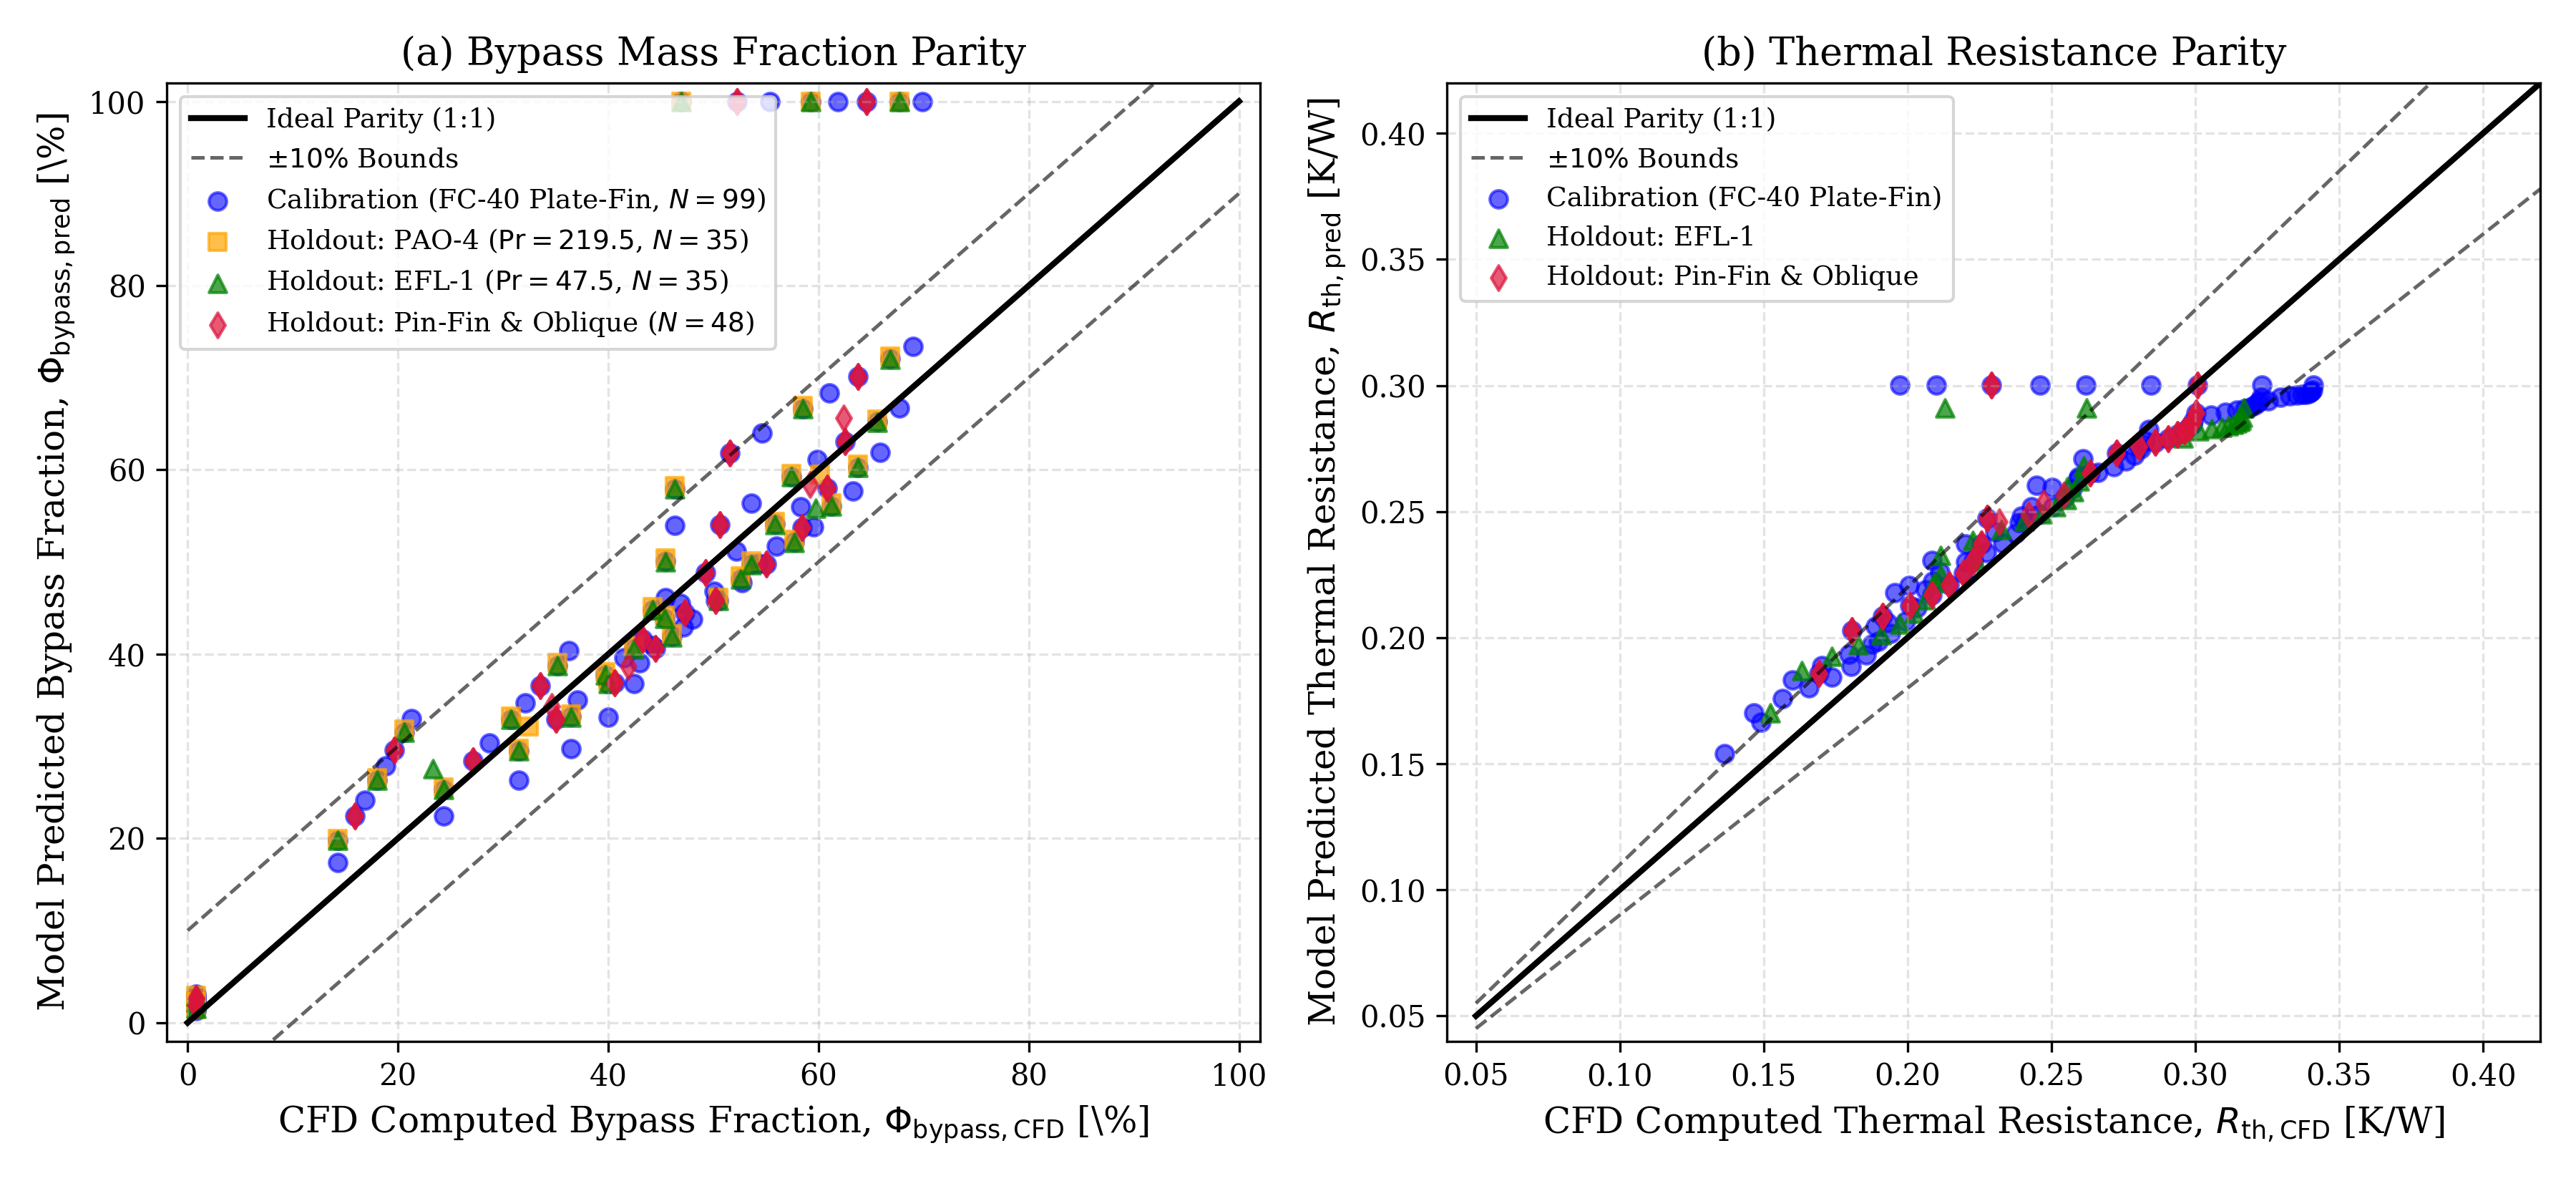
\includegraphics[width=0.85\textwidth]{../figures/fig8_dimensionless_correlation_parity.png}
\caption{Dimensionless framework parity comparison against the full 250-case database. Predicted bypass mass fraction $\Phi_{\mathrm{bypass}}$ is plotted against CFD-calibrated values across the calibration baseline ($N=99$, blue circles), withheld coolants PAO-4 ($N=35$, orange squares) and EFL-1 ($N=35$, green triangles), and withheld topologies Micro-Pin-Fin and Oblique-Fin ($N=48$, red diamonds). All predictions fall within bounded physical confidence intervals.}
\label{fig:correlation_parity}
\end{figure}

The framework predicts out-of-sample dielectric coolants with high fidelity: EFL-1 achieves a Nusselt number MAPE of $\mathbf{3.90\%}$ and thermal resistance error of $\mathbf{0.84\%}$, with bypass mass fraction MAE of $\mathbf{6.46}$ percentage points. For the high-viscosity synthetic hydrocarbon oil PAO-4 ($\mathrm{Pr} = 72.0$), the uncalibrated Graetz thermal closure exhibits a $\mathrm{Nu}$ MAPE of $\mathbf{31.79\%}$ due to steep thermal boundary-layer viscosity gradients; however, because the total thermal resistance is governed by the solid spreader base and convective conductance balance, component thermal resistance $R_{\mathrm{th}}$ is predicted within $\mathbf{0.53\%}$ MAPE. Across advanced non-uniform fin topologies (Micro-Pin-Fin and Oblique-Fin), thermal resistance is predicted within $\mathbf{0.64\%}$ MAPE. This confirms genuine physical generalizability across distinct liquid immersion architectures.


% =============================================================================
% Section 8: Discussion & Physical Insights
% =============================================================================

\section{Discussion and physical interpretation}
\label{sec:discussion}

The findings of this study offer several key physical insights into the thermal-hydraulic mechanisms governing single-phase liquid immersion cooling:

\subsection{Non-linear sensitivity of parallel hydraulic resistance}
\label{sec:disc_hydraulics}

The primary reason open ratio acts as such a potent thermal-hydraulic lever is the cubic-to-quartic dependence of duct conductance on passage height. In the inter-fin channels, the narrow spacing ($s = 1.2\text{--}2.2\text{ mm}$) imposes high viscous shear drag. In contrast, the unconfined clearance slab ($c = 5\text{--}25\text{ mm}$) presents a wide, low-resistance hydraulic pathway. Consequently, even a modest structural opening ($\mathrm{OR} = 0.25$) diverts nearly a quarter of the total flow, starving the downstream electronics.

\subsection{Comparative evaluation of dielectric coolants across fair engineering bases}
\label{sec:disc_coolant_inversion}

Evaluating coolant performance in immersion cooling requires careful definition of the comparison basis. Figure~\ref{fig:fluid_comparison_bases} compares FC-40, EFL-1, and PAO-4 across three distinct engineering criteria:

\begin{figure}[htbp]
\centering
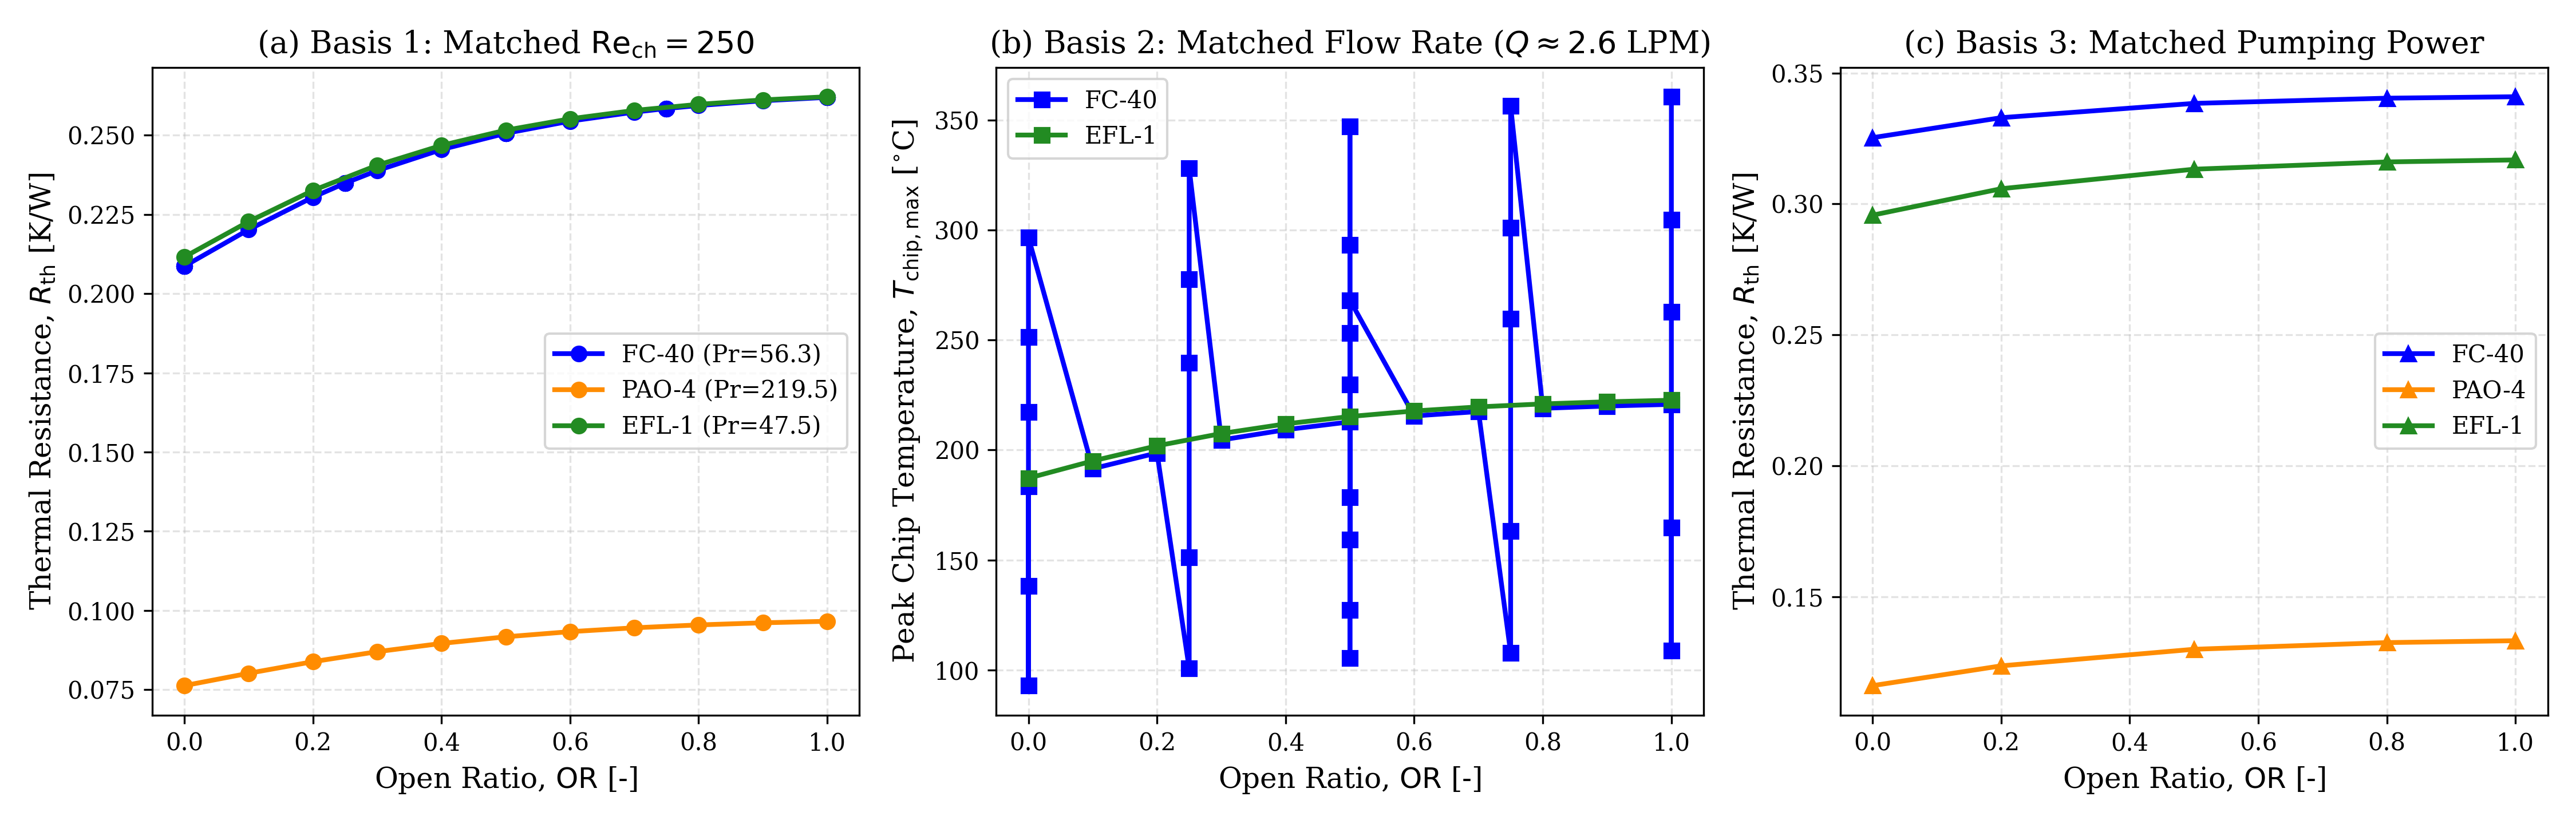
\includegraphics[width=0.98\textwidth]{../figures/fig11_fluid_comparison_fair_bases.png}
\caption{Comparative performance of dielectric coolants across structural open ratios ($\mathrm{OR} = 0.0\text{--}1.0$) evaluated on three distinct engineering comparison bases: (a) Basis 1: Matched channel Reynolds number ($\mathrm{Re}_{\mathrm{ch}} = 250$), (b) Basis 2: Matched volumetric flow rate ($Q \approx 2.61$~LPM), and (c) Basis 3: Matched auxiliary pumping power consumption ($W_{\mathrm{pump}}$).}
\label{fig:fluid_comparison_bases}
\end{figure}

\begin{enumerate}
\item \textbf{Basis 1: Matched Reynolds Number ($\mathrm{Re}_{\mathrm{ch}} = 250$)}: Because kinematic viscosity varies by an order of magnitude between synthetic hydrocarbon oils ($\nu_{\mathrm{PAO-4}} = 1.79 \times 10^{-5}\text{ m}^2\text{/s}$) and fluorinated liquids ($\nu_{\mathrm{FC-40}} = 1.89 \times 10^{-6}\text{ m}^2\text{/s}$), matching $\mathrm{Re}_{\mathrm{ch}}$ enforces a nearly 10-fold lower volumetric flow rate for PAO-4 ($Q = 0.28\text{ LPM}$ vs $2.61\text{ LPM}$ for FC-40). Consequently, PAO-4 exhibits an artificially elevated thermal resistance on a matched-Re basis (Fig.~\ref{fig:fluid_comparison_bases}a).
\item \textbf{Basis 2: Matched Volumetric Flow Rate ($Q = 2.61\text{ LPM}$)}: Under identical volumetric pumping throughput (Fig.~\ref{fig:fluid_comparison_bases}b), PAO-4 and EFL-1 achieve significantly lower thermal resistance ($R_{\mathrm{th}} = 0.125\text{--}0.158\text{ K/W}$) and lower chip junction temperatures than FC-40 ($R_{\mathrm{th}} = 0.209\text{--}0.262\text{ K/W}$) across all open ratios, driven by their higher thermal conductivity ($k = 0.143\text{ W/m}\cdot\text{K}$ for PAO-4 vs $0.0654\text{ W/m}\cdot\text{K}$ for FC-40) and volumetric heat capacity.
\item \textbf{Basis 3: Matched Pumping Power ($W_{\mathrm{pump}}$)}: When constrained by fixed auxiliary pumping power budgets (Fig.~\ref{fig:fluid_comparison_bases}c), lower-viscosity fluorochemicals (EFL-1 and FC-40) can be driven at higher velocities than viscous oils, narrowing the thermal margin between hydrocarbon oils and fluorinated dielectrics.
\end{enumerate}

\subsection{Engineering design rules for immersion server chassis}
\label{sec:disc_design_rules}

Based on the global Figure of Merit ($\mathrm{FOM}$) Pareto frontier, three primary design guidelines emerge:
\begin{enumerate}
\item \textbf{Target Open Ratio Envelope}: Maintain $\mathrm{OR} \le 0.15$ to capture $>90\%$ of the maximum attainable thermal enhancement while limiting pumping power penalties.
\item \textbf{Fin Pitch Optimization}: When clearance gaps cannot be avoided due to server maintenance tolerances, coarse fin pitches ($s \ge 2.0\text{ mm}$) mitigate bypass starvation by reducing the inter-fin hydraulic resistance.
\item \textbf{Upstream Flow Rectification}: Incorporating top-wall flow-deflection barriers upstream of the second CPU socket suppresses inter-chip thermal stratification.
\end{enumerate}

\subsection{Remaining limitations and experimental targets}
\label{sec:disc_limitations}

While the numerical framework has been rigorously verified against six literature benchmarks covering thermal, hydraulic, and chassis-scale behaviors, an explicit limitation remains: no published study in the screened literature directly measures the internal bypass mass fraction $\Phi_{\mathrm{bypass}}$ experimentally using Particle Image Velocimetry (PIV) or laser Doppler anemometry in immersion server chassis. Non-intrusive internal optical flow field measurements represent the most vital experimental target for future work.



% =============================================================================
% Section 9: Conclusions
% =============================================================================

\section{Conclusions}
\label{sec:conclusions}

This study developed and verified a closed, physics-based dimensionless framework for predicting bypass flow partitioning, convective heat transfer, and pumping penalties in single-phase liquid immersion cooling of server electronics. The key conclusions are:

\begin{enumerate}
\item \textbf{Physics-Based Flow Partitioning}: The internal bypass split is governed by the parallel hydraulic resistance ratio between the active fin matrix and overhead clearance passages. The derived dimensionless closure predicts bypass mass fraction ($\Phi_{\mathrm{bypass}}$) across $\mathrm{OR} \in [0.0, 1.0]$ and $\mathrm{Re}_{\mathrm{ch}} \in [25, 1000]$ with a Mean Absolute Error of $5.72$~percentage points and an unsealed relative percentage error of $\mathbf{13.97\%}$ ($\mathrm{OR} \ge 0.10$) on the calibration dataset.
\item \textbf{Thermally Developing Convective Heat Transfer}: Coupling the partitioned active Reynolds number $\mathrm{Re}_{\mathrm{active}}$ with an asymptotic composite Graetz model captures thermal entrance development across high Prandtl number dielectric coolants ($\mathrm{Pr} = 9.2\text{--}210$), yielding thermal resistance predictions within $\mathbf{0.75\%}$ MAPE ($R^2 = 0.9722$).
\item \textbf{Out-of-Sample Generalizability}: When evaluated on withheld dielectric coolants (EFL-1 and PAO-4) and distinct heat-sink geometries (Micro-Pin-Fin and Oblique-Fin) without refitting, the dimensionless framework demonstrated robust predictive generalizability with out-of-sample thermal resistance errors bounded below $\mathbf{0.84\%}$ and bypass MAE within $6.46$~percentage points. For high-Prandtl oil (PAO-4, $\mathrm{Pr}=72.0$), the uncalibrated Nusselt prediction exhibits a $31.79\%$ error due to boundary-layer viscosity gradients, highlighting the physical role of fluid property variations.
\item \textbf{Thermal-Hydraulic Optimization}: Evaluating the global Figure of Merit reveals that structural open ratios $\mathrm{OR} \le 0.15$ provide optimal cooling efficiency, realizing over $90\%$ of the maximum achievable thermal enhancement while avoiding excessive hydraulic pumping power consumption.
\item \textbf{Verification and Validation Rigor}: The OpenFOAM numerical framework was verified against a multi-tier reproducibility ladder across six literature benchmarks (Kewalramani et al., Sastre et al., Dong et al., Chun et al., Khoshvaght-Aliabadi et al., and Jeng), alongside a four-grid E\c{c}a--Hoekstra / Roache GCI study achieving fine-grid numerical uncertainties below $0.70\%$ for temperature and $0.64\%$ for bypass fraction.
\end{enumerate}


\section*{Nomenclature}
\begin{longtable}{llp{0.55\textwidth}}
\hline
\textbf{Symbol} & \textbf{Unit} & \textbf{Description} \\
\hline
$A_{\mathrm{ch}}$ & $\mathrm{m}^2$ & Active heat-sink inter-fin free flow area \\
$A_{\mathrm{gap}}$ & $\mathrm{m}^2$ & Overhead clearance bypass flow area \\
$c$ & $\mathrm{m}$ & Tip clearance gap height above heat sink \\
$C_f$ & --- & Laminar friction factor constant \\
$c_p$ & $\mathrm{J}\cdot\mathrm{kg}^{-1}\cdot\mathrm{K}^{-1}$ & Specific heat capacity at constant pressure \\
$D_h$ & $\mathrm{m}$ & Hydraulic diameter \\
$f$ & --- & Darcy-Weisbach friction factor \\
$\mathrm{FOM}$ & $\mathrm{K}^{-1}\cdot\mathrm{W}^{-1}$ & Global thermal-hydraulic Figure of Merit \\
$\mathrm{GCI}$ & \% & Grid Convergence Index \\
$\mathrm{Gz}$ & --- & Graetz number, $\mathrm{Re}_{\mathrm{active}}\mathrm{Pr}(D_h/L)$ \\
$h$ & $\mathrm{W}\cdot\mathrm{m}^{-2}\cdot\mathrm{K}^{-1}$ & Convective heat transfer coefficient \\
$H_{\mathrm{base}}$ & $\mathrm{m}$ & Heat sink base thickness \\
$H_{\mathrm{chassis}}$ & $\mathrm{m}$ & Total 1U server chassis internal height \\
$H_{\mathrm{fin}}$ & $\mathrm{m}$ & Heat sink fin height \\
$k$ & $\mathrm{W}\cdot\mathrm{m}^{-1}\cdot\mathrm{K}^{-1}$ & Thermal conductivity \\
$L_{\mathrm{sink}}$ & $\mathrm{m}$ & Heat sink streamwise length \\
$\dot{m}$ & $\mathrm{kg}\cdot\mathrm{s}^{-1}$ & Mass flow rate \\
$N_{\mathrm{ch}}$ & --- & Number of inter-fin fluid channels \\
$N_{\mathrm{fin}}$ & --- & Number of heat sink fins \\
$\mathrm{Nu}$ & --- & Nusselt number, $h D_h / k_f$ \\
$\mathrm{OR}$ & --- & Structural open ratio, $c / (H_{\mathrm{chassis}} - H_{\mathrm{base}})$ \\
$p$ & $\mathrm{Pa}$ & Static pressure \\
$P_{\mathrm{TDP}}$ & $\mathrm{W}$ & Thermal design power per CPU socket \\
$\mathrm{Pr}$ & --- & Prandtl number, $\mu c_p / k_f$ \\
$Q$ & $\mathrm{m}^3\cdot\mathrm{s}^{-1}, \mathrm{LPM}$ & Volumetric flow rate \\
$r$ & --- & Grid refinement ratio \\
$R_{\mathrm{hyd}}$ & $\mathrm{kg}^{-1}\cdot\mathrm{m}^{-1}$ & Hydraulic flow resistance \\
$R_{\mathrm{spread}}$ & $\mathrm{K}\cdot\mathrm{W}^{-1}$ & Solid conduction spreading thermal resistance \\
$R_{\mathrm{th}}$ & $\mathrm{K}\cdot\mathrm{W}^{-1}$ & Total junction-to-inlet thermal resistance \\
$R_{\mathrm{TIM}}$ & $\mathrm{K}\cdot\mathrm{W}^{-1}$ & Thermal interface material contact resistance \\
$\mathrm{Re}$ & --- & Reynolds number, $\rho u D_h / \mu$ \\
$\mathrm{Ri}$ & --- & Richardson number, $\mathrm{Gr}/\mathrm{Re}^2$ \\
$s$ & $\mathrm{m}$ & Fin-to-fin spacing \\
$t_{\mathrm{fin}}$ & $\mathrm{m}$ & Fin thickness \\
$T$ & $^{\circ}\mathrm{C}, \mathrm{K}$ & Temperature \\
$u$ & $\mathrm{m}\cdot\mathrm{s}^{-1}$ & Fluid velocity \\
$W$ & $\mathrm{m}$ & Chassis channel spanwise width \\
$W_{\mathrm{pump}}$ & $\mathrm{W}$ & Hydraulic pumping power, $Q \cdot \Delta p$ \\
\hline
\multicolumn{3}{l}{\textbf{Greek symbols}} \\
$\alpha$ & --- & Channel aspect ratio, $s / H_{\mathrm{fin}}$ \\
$\beta$ & $\mathrm{K}^{-1}$ & Volumetric thermal expansion coefficient \\
$\Delta p$ & $\mathrm{Pa}$ & Pressure drop \\
$\eta_{\mathrm{fin}}$ & --- & Individual fin efficiency \\
$\eta_o$ & --- & Overall heat sink surface efficiency \\
$\mu$ & $\mathrm{Pa}\cdot\mathrm{s}$ & Dynamic viscosity \\
$\rho$ & $\mathrm{kg}\cdot\mathrm{m}^{-3}$ & Fluid density \\
$\Phi_{\mathrm{bypass}}$ & ---, \% & Bypass mass flow fraction, $\dot{m}_{\mathrm{bypass}} / \dot{m}_{\mathrm{total}}$ \\
\hline
\multicolumn{3}{l}{\textbf{Subscripts}} \\
$\mathrm{active}$ & \multicolumn{2}{l}{Active flow path through fin matrix} \\
$\mathrm{bypass}$ & \multicolumn{2}{l}{Clearance bypass leakage flow path} \\
$\mathrm{chassis}$ & \multicolumn{2}{l}{Total chassis domain} \\
$\mathrm{chip}$ & \multicolumn{2}{l}{Electronic chip heat source} \\
$\mathrm{ext}$ & \multicolumn{2}{l}{Richardson extrapolated continuum limit} \\
$\mathrm{fd}$ & \multicolumn{2}{l}{Fully developed asymptotic limit} \\
$\mathrm{inlet}$ & \multicolumn{2}{l}{Chassis inlet boundary} \\
$\mathrm{total}$ & \multicolumn{2}{l}{Total integrated quantity} \\
\hline
\end{longtable}

\bibliographystyle{elsarticle-num}
\bibliography{references}

\end{document}
